\svnkwsave{$RepoFile: siminos/spatiotemp/chapter/blogMNG17.tex $}
\svnidlong {$HeadURL: svn://zero.physics.gatech.edu/siminos/spatiotemp/chapter/blogMNG17.tex $}
{$LastChangedDate: 2020-04-19 01:28:36 -0400 (Sun, 19 Apr 2020) $}
{$LastChangedRevision: 6859 $} {$LastChangedBy: predrag $}
\svnid{$Id: blogMNG17.tex 6859 2019-05-09 20:51:31Z predrag $}

\chapter{Matt's 2017 blog}
\label{chap:blogMNG17}
% Predrag                                           1 May 2018

\begin{description}

\MNGpost{2017-02-13}{
\begin{description}
\item[Inertial manifold dimension]
Installed Channelflow to terminal in Howey, wrote and currently
running scripts to automatically compute Floquet vectors generated via Arnoldi iteration at 256 points
around the shortest periodic orbit of the HKW (Hamilton, Kim, Waleffe) minimal flow unit. Split into
four tasks and hopefully my crude script writing hasn't overlooked anything. Will probably run for
a couple of days.

More details: Using 100 arnoldi iterations to produce all unstable and marginal eigenvectors, in addition to
50 stable eigenvectors. I'm hoping 100 iterations is enough for convergence, seems
to be from preliminary tests in Cali.

\item[Fritz John PDE book]
On order from library, should arrive tomorrow.

\item[Variational multishooting]
Still trying to implement adjoint equation.
\end{description}
}

\MNGpost{2017-02-15}{:
\begin{description}
\item[Variational multishooting]
I have implemented all of the pieces, but it seems to share some of the bad
behavior that I encountered when implementing the variational {\descent},
the problem is that I do not know how to compensate for this unlike the other
time, as there isn't much wiggle room other than increasing the discretization
or the number of integrations steps in the shooting process. I think the problem
is due to the ability of allowing the shooting times to vary independently of
one another. Either way, it seems to run much slower than what I already have
so I think I will shelve this idea for now, as it is much more important to use
what I am comfortable with to produce tori than discuss and investigate the
differences between numerical methods. (The other investigation would be modified
Newton with trust region that John Gibson talked to Ashley Willis and I about). I personally
think conjoining Krylov subspace methods with the variational {\descent} is the
way to go.

\item[Fritz PDE]
Read the first chapter (of four total) of the partial differential equations book.
It went over the method of characteristics for first order equations. It seems
to pick up in the next chapter so I'm excited to see where this leads.

\item[Guckenheimer and Holmes]
Picked up this book via suggestion of Burak
\end{description}
}

%look to dimension.tex in pipes
%\begin{figure}[ht]
%\centering
%\includegraphics[width=0.9\textwidth]{MNGp19p02_12}
%\caption{\label{fig:MNGIP12}
%Pairwise angles between Floquet vectors corresponding to the two
%most unstable Floquet exponents $\lambda_{\pm} = 0.026566170899604846 \pm
%0.028912315120577528i$. These angles were evaluated by computing the $L2$ %inner product
%of the corresponding Floquet vectors
%at $256$ discretized points around the shortest known periodic orbit of %the HK3 cell %p19p02 in Channelflow notation
%}
%\end{figure}

\MNGpost{2017-02-16}{
\begin{description}
\item[Pairwise angles]
Spent most of the day trying to figure how to correctly write bash scripts in linux, and
how to apply them to Channelflow.
Uploading first results from pairwise angle calculations of Floquet vectors for Channelflow.
Rereading about how to move onto principal angles between linear subspaces as was done in \refref{DCTSCD14}
\end{description}
}

\MNGpost{2017-02-21}{
\begin{description}
\item[Spatial {\descent}]
Debugging and changing spatial {\descent} code. I think I've pinned down the main problem
to be an error in trying to use Fourier transforms rather than explicit sums in my definition
for the stability matrix elements, or initial condition generation. I'm currently using the
shortest periodic orbit in time as an initial guess; Therefore, I would expect the value
of the cost functional to be small relative to something that isn't already doubly-periodic
in time and space. While the value of the cost functional is relatively small, it still may
be too large for an initial guess.

That being said I can at least list what I believe to be the most likely cause of errors.
\begin{itemize}
\item Error in definition of stability matrix elements; this can be seen from the inability of
the fictitious time evolution to lower the value of the cost functional.
\item Poor initial conditions, in a specific sense. I think a periodic orbit is a good start, but
the number of Fourier modes kept or discretization in space might be impeding progress; One problem
is memory requirements due to having a system of equations for spatial derivatives as opposed to a
single ODE prevents large discretizations.
\end{itemize}

\item[Fritz PDE]
It's taking a while to digest; There are a lot of geometrical notions about solutions to PDEs that
I have never really considered before. Apparently cones are much more abundant that I would have
previously believed.

\end{description}
}

\MNGpost{2017-02-21}{
\begin{description}
\item[spatial {\descent}]
Put a lot of time into debugging spatial {\descent} code. Due to size of
the system it takes much longer to run than antisymmetric subspace
$\bbU^+$ calculations making it more time consuming to check to see if
its running properly. Currently I am able to take initial conditions with
initial value of cost functional $\mathcal{F}^2 \approx 150$ to a final
value of $\mathcal{F}^2 \approx 10^{-5}$. This leads me to believe I have
caught most of the small errors and only have a little bit more work into
finding what I am overlooking before it will be fully operational (if I
may be so bold as to sound like an engineer).

One of the main problems I have been having is that the fictitious time evolution is much more
temperamental; increasing step sizes seems to be much more "unstable" in the sense that even
when close to (spatially) periodic solutions it is still possible to overshoot and therefore
ruin the run. In order to combat this I am going to make a run on Light with much smaller step
sizes than I would normally use, and let it run overnight.

\item[Fourier differentiation for later use]
I also have been playing around with using Fourier series (spectral differentiation) as a means
to calculate the approximate tangent space. As one would expect, it is much faster than multiplying
a large matrix (finite differencing scheme) with a large vector (Approximately 100 times faster), but
there I am somewhat confused on how to include this into the matrix equation \refeq{e-MNGVND}
that is the meat of
the computation process, without completely rewriting my code.

The reason for this is such: Spectral differentiation with respect to a parameterization variable,
$s$, can be rewritten as multiplication by a diagonal matrix with elements $is$, but this requires
the vector that is representing the entire loop to be ordered in a very specific way. If the loop
was ordered in this specific way it would reduce to multiplication of a large diagonal matrix which would
be repeating the (small) diagonal matrices with elements $is$. If one wants to do it this way I believe
the easiest way, in order to avoid reordering the stability matrix elements, would be to formulate it
this way mathematically: The matrix $D_{\mathcal{F}}$, which produces the approximate tangent space
after multiplication with the "loop vector" $\mathbf{x}$, could be represented in such a way,

\beq \nonumber
D_{\mathcal{F}} = \mathbf{P}^{-1}\mathbf{F}^{-1}\mathbf{Diag}(is)\mathbf{F}\mathbf{P} \quad
    \mbox{where,}
\label{e-FvndBAD}
\eeq
$\mathbf{F}$ = Block diagonal matrix composed of Fourier transform matrices (i.e. to Fourier transform each
of the Fourier coefficient series with respect to parameterization variable), $\mathbf{P}$ = Permutation matrix
to reorder in specific way to enable easy Fourier transforms.

This is probably too convoluted as it is somewhat hard to explain, but keeping a record for future
possible implementations.

\end{description}
}

\MNGpost{2017-02-22}{
\begin{description}
\item[Checklist]
Modifying and relocating checklist from before to correctly denote what is currently being accomplished
for finding principal angles of subspaces for channel flow.

%boxes to be filled with 'x' and dated when completed. Checklist is subject to change
\item[[x]] \MNGedit{1-24-2017} Generate time discretized periodic orbit using Channelflow.
\item[[x]] \MNGedit{2-2-2017} Use Arnoldi iteration to find eigenfunctions of periodic orbits
\item[[x]] \MNGedit{2-13-2017}Produce eigenfunctions around periodic orbit in an \emph{automatic} rather than manual fashion
\item[[x]] \MNGedit{2-16-2017}Compute $L2$ pairwise norms of eigenfunctions as first measure of angles.
\item[[]] Compute principal angles between subspaces of eigenfunctions.

\item[Principal angles]
Here is a description that I am trying to implement in c++ in order to work with Channelflow, this corresponds to the
last step in the checklist, but has multiple steps itself.

Procedure taken from \refref{BjoGol73}:
\item[[]] For the nth subspace, form two matrices A, B such that $Range(A) = span{e_1, ..., e_n},
            Range(B) = span{e_{n+1}, ... , e_N}$, $e_k = k^{th} eigenvector$
\item[[]] Use Eigen c++ package to perform Householder triangularization to produce QR decompositions of A and B.
\item[[]] Form matrix $M = Q_A{\dagger}Q_B$ and apply c++ JacobiSVD on it to get principal values $\sigma_k$
\item[[]] $\sigma_k$ from previous step = $\cos \theta_k$ where $\theta$ is the principal angle between the $k$th subspace of A,B.
          (only care about the first principal angles, not orthogonal complements).

\item[spatial {\descent}]
Bad results from overnight trial; stalls out around
cost functional value $\mathcal{F}^2 \approx 10^{-8}$. Final configuration
space velocity field is a highly oscillating very non-physical
 type solution that looks like the result of aliasing; I believe I need
to incorporate more Fourier modes as a first step to fix the
 issue, or the number of discretization points, although doing so leads me
to run out of memory

\textbf{After talking to PC today he pointed out that
this is likely due to forgetting to slice the orbit; Need to do this with {\fFslice}}.

\item[Reading]
Read a little bit more of Fritz, linear subspace
angles\rf{BjoGol73}, symmetry reduction\rf{BudCvi14}

\item[Xiong's comments]
Xiong really thinks that in order to get anything meaningful I
need to find Floquet vectors along all possible periodic orbits, as
well as orbits that shadow these orbits.

\item[updates]
Updated codes to svn, updated pairwise angle figure from feb 16th.

\item[arnoldi iteration]
Getting more Floquet vectors from periodic orbits from Channelflow database; there seems to be a problem this time around.
Background of the problem:
before arnoldi iteration proceeds, the arnoldi program of Channelflow
computes the $L2$ norm of $\sigma f^{T}(u)-u$ and
warns if it is greater than $10^-8$; for the first point on the orbit
this time around this error is $10^{-10}$ but for other
points it's $\approx 10^{-1}$. Need to figure out what is causing
this discrepancy. The first thing that this points to is that
the DNS of the periodic orbit is unstable and I need to go back
and decrease the step size, but the step size was already smaller
than the default when I generated the data in the first place.


\end{description}
}

\item[Xiong to Matt 2017-02-23]
With only a few {\po}s, I think it may be easier to check the local Floquet
exponents first. They are defined as
\beq
  \lambda_{j}(\ssp)
  = \transp{\bm{e}_j(\ssp)}D(\ssp)\,\bm{e}_j(\ssp)
  = \lim_{\tau\rightarrow 0}\frac{1}{\tau}\ln ||J^\tau(\ssp)\bm{e}_j(\ssp)||
  \,.
\ee{XiongNotAgain}
$D$ is the strain tensor $D = (\Mvar + \transp{\Mvar})/2$ with $\Mvar$ the
stability matrix. It may be hard to obtain the transpose of $\Mvar$, but we
can evolve the Floquet vectors $\bm{e}_j(\ssp)$ (of the full cycle) by the
\jacobianM\ for a short time to get the instantaneous expansion/contraction
rates. \reffig{fig:localFErpo1} shows the local Floquet exponents for
\RPO{16.31} in \KSe. There is a clearly separation between the leading
8 modes and the rest. Maybe you can observe similar phenomenon in the channel
flow. That will give an estimate of the dimension.
%look to dimension.tex in pipes
%\begin{figure}[h]
%  \centering
%  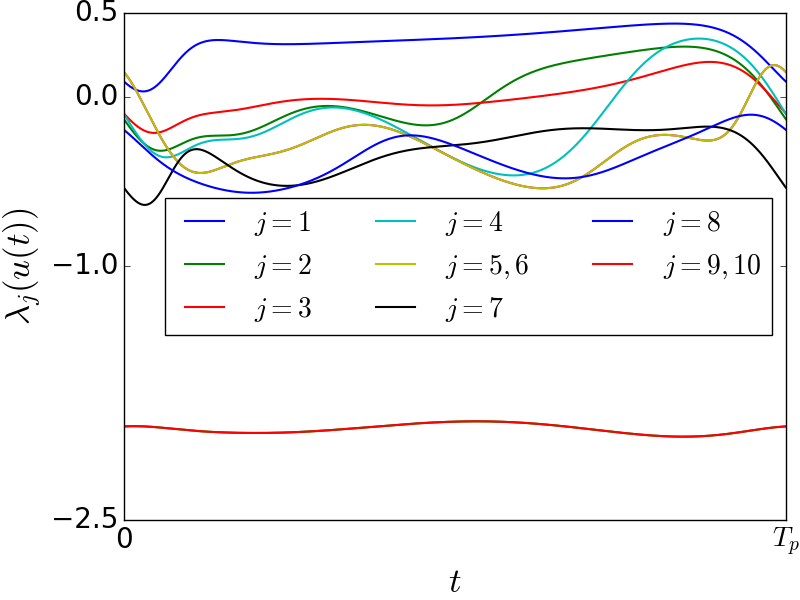
\includegraphics[width=0.7\textwidth]{localFErpo1}
%  \caption{
%    The leading 10 local Floquet exponents for \RPO{16.31} in KS %equation.}
%  \label{fig:localFErpo1}
%\end{figure}

\PCpost{2017-02-23}{
``Local Floquet exponents'' are back? This is like calling function $f(\ssp)$
``local integral''
\[
\lim_{\ssp''\to\ssp} \frac{1}{\ssp''-\ssp}\int_\ssp^{\ssp''}\!\!d\ssp'f(\ssp')
\,.
\]
$\Mvar(\ssp)$ is $d$\dmn\ generalization of $dv(\ssp)/d\ssp$, and that is an
object that is not invariant under general nonlinear coordinate transformations.
The value of such derivative could be anything - the only meaningful quantity
is the spectrum of the Floquet matrix, which is invariant.
There is no reason to give any particular significance to
\[
  \transp{\bm{e}_j(\ssp)}D(\ssp)\,\bm{e}_j(\ssp)
  = \transp{\bm{e}_j(\ssp)}\Mvar(\ssp)\,\bm{e}_j(\ssp)
\]
and one does not need to evaluate $\transp{\Mvar}$, as the transpose of
a scalar is itself,
\[
\transp{(\transp{\bm{e}_j}\Mvar\,\bm{e}_j)}
=
\transp{\bm{e}_j}\transp{\Mvar}\,\bm{e}_j
\,.
\]
We put up with this nonsense in \refref{DCTSCD14} only in order to finally
get the paper submitted - it is not my job to teach adult collaborators
nonlinear dynamics, if they are unwilling to learn. Grad students - that's
different.
Oscillations in \refeq{XiongNotAgain} happen to be mild, but we have no
argument that they should be mild. That's fortuitous.
}

\item[Xiong to Predrag 2017-02-23] Yes, you are right. We do not
need $\transp{A}$ get the instantaneous expansion/contraction rate.
But it is required in the definition because
 $\transp{\bm{e}_j}\transp{\Mvar}\,\bm{e}_j$ is a complex number
for complex vectors. I do not think that such an
instantaneous rate is nonsense. The idea is backed by the domination of
Oseledec splitting. Experiments with \cGLe\ with \cLvs\ also
use this idea. For now, if we do not have enough orbits to study
the principle angles statistically, why not try to have a look at
local Floquet exponents? Maybe it gives us some intuition.

\MNGpost{2017-02-23}{:
\begin{description}
\item[J. Demmel talk]
\textit{Communication-Avoiding Algorithms for Linear Algebra and Beyond}
\HREF{https://people.eecs.berkeley.edu/~demmel}{(Link with Slides)}
\HREF{https://bebop.cs.berkeley.edu}{(Additional Info)}

Motivation is that algorithms have two costs, flops and moving data.
Counting costs, flops measured in time per flop, "words moved" measured in
bandwidth, messages (described as groups of "words") measured by latency.

Minimize communications to save energy.

Redesign algorithms to avoid communication, between all memory hierarchy levels. Obtain
lower bounds if possible.

Some Numbers:
12 times faster matrix multiplication (on 64 thousand cores)
 (doesn't scale too well, larger matrices achieve
only something like 2.7 times)
3 times faster tensor contractions

Outline of Communication-Avoiding (CA) algorithms.

Survey of CA Linear Algebra
Direct Linear algebra, lower bounds on communication on $Ax=b$, $Ax= \lambda x$, least squares, svd.
being added to LAPACK, PLASMA, MAGMA.

Lower bound on Bandwidth cost for all $n^3$ like (three nested loops) linear algebra.
Let M = fast memory size per processor
Lower bound
Words\_moved(per processor) = $\mathcal{O}$( flops(per proc) / $M^{1/2} )$

``When can you obtain this lower bound in sparse case?"
(not considering things like diagonal matrix multiplication which is highly optimized)

Lower bound on the Latency cost
\\words\_moved(per processor) = flops(per processor)/ $M^{3/2}$


Naive intro to linear algebra, matrix multiplication with three loops.

Split matrices into $b \times b$
How big should b, be?
Need b sized blocks to fit into fast memory, lower bound of $flops/M^1/2$

Parallel matrix multiplication,
Break matrix into small submatrices.

Summary of dense parallel algorithms attaining communication lower bounds.
obtain lower bounds with lower bounds of messages and words. (with b constant).

Algorithms have been optimized to follow, but there is an additional step of
optimization with regards to the memory size M.
"Can we always hit the lower bound no matter how much memory there is?" yes.


12 times factor of speeding up is due to a 95 percent reduction in communication time
Algorithm was sold to company that was later acquired by intel.

Same thing with Tall-skinny QR.
Break into blocks, do local QR decomposition. break into smaller and smaller blocks
via repeated QR. (MPI reduce).

"how does this affect the stability?"
QR: only use multiplication by orthogonal matrices, still works.
When abandoning partial pivoting had to prove stability (which was proved in an
unreferenced paper).

Where do $M^{1/2}$ come from in the lower bounds: generalization of lower bounds
General case of matrix multiplication, as many indices as you want. only really need the
indices.

Access locations indexed by group homomorphisms, maps list of indices
to specific matrix element?

Ongoing: Implement and improve algorithms to generate lower bounds, optimal algorithms.
Extend speedups by using extra memory $(n+1/2)$ dimension algorithms

Krylov subspace methods
(Arnoldi, Lanczos, CG, GMRES)
Assume matrix well-partitioned.
Serial implementation: (k sparse matrix multiples. moves slow to fast memory)
New case: read from slow memory to fast memory \textbf{once}
parallel implementation on p processors: price we pay is some redundant computation
(flops are cheap).
Challenges: Poor partition, preconditioning, num. stability.

Instead of using monomial basis, use a "Newton basis" for CA-GMRES to achieve same
convergence properties of GMRES.

\end{description}
}

\MNGpost{2017-02-24}{:
\begin{description}
\item[S. Berman Math Colloquium]
\textit{A classical Hamiltonian model for HHG}
High Harmonic Generation, send in intense laser pulse into gas,
focused in directions transverse to propagation.

Measured the transmitted light, the spectrum typically is composed
of three distinct behaviors for intensity as a function
of frequency, monotonic decrease, plateau, and then convergence
to zero. Interested in plateau region in a classical sense.

Introducing an electric field description for the incident light.
Radiation from incident light interacting with gas. Main goal
is to try to describe plateau region classically.

The basis for the classical model is to assume there are N single electron
atoms indexed by position. Assume ions do not interact with each other, and
therefore there is only potential due to the interactions between atoms and
their electrons. Therefore, the different ions will interact indirectly through
the electric and magnetic fields.

Have a set of ODEs that come from Lorentz force law and Maxwell's equations.
Has a Hamiltonian structure, want to try and preserve this structure.

Defines a Hamiltonian and the derived Poisson Bracket.
Need a finite discrete implementation that captures all of the Physics.

Reduction of the Hamiltonian by defining a periodic box such that one
can Fourier transform in all three spatial coordinates. Find expressions
for Functional derivatives that were present in Poisson Bracket, i.e.
trying to get expressions for dynamical equations in Fourier space.

Make linear transformations that eliminate trivial time dependence,
changes the Hamiltonian to look like harmonic oscillator, and modifies
the poisson bracket but still satisfies Jacobi identity.

This transformed system still isn't tractable due to its size. Doesn't
take into consideration ionization, but theory predicts comoving electric
fields so that you only care about electric field in a small box.
\end{description}
}

\MNGpost{2017-02-27}{:
\begin{description}
\item[spatial {\descent}]
Further changes to spatial code, yielding equilibria in time. Previously
when I was working with antisymmetric subspace $\bbU^+$ in time, this
typically indicated that there was some mistake with a numerical factor
somewhere, but here I am not so sure as it is still a periodic orbit in
space. Although, if I had to wager, it would be a mistake that I'm
looking over somewhere.

Another main challenge is how to implement a slice condition to deal with translational
invariance. Typically this is dealt with when the spatial Fourier series is being used, and
therefore it is easier to represent a hypersurface that eliminates this marginal direction; in
the spatial {\descent} code (this is what I call using \refeq{e-FksX} with variational {\descent}) I am trying to eliminate the translational freedom but it's not as straightforward as
the {\fFslice}; as the {\fFslice} in this case would eliminate time translations.
I've been looking towards some of the papers about invariant tori and their "phase conditions" as a
possible means of escape.


\item[Floquet vectors]
I've been having a problem with computing the Floquet vectors associated with {\rpo}s.

I produce a discretized periodic orbit by using Channelflow's DNS, while restricting solutions
to remain in their symmetry subspace as dictated by the symmetries listed in the data base at
\HREF{www.Channelflow.org}{(Channelflow)}. Then at each of these discretized points along the
periodic orbit, I begin arnoldi iteration. One of the first checks of the arnoldi iteration verifies
whether $\sigma f^T (u) - u \approx 0 $, as this is what dictates a relative periodic solution.
Now, the problem is that for the first point
of the discretization (i.e. the initial condition taken from the database, $u_0$ ),
$\sigma f^T(u_0) - u_0 \approx 10^{-8}$, but for any other point of the discretization, the error
is more like $10^{-1}$, which is unacceptable as it means we've somehow been set off course. At first
I thought this doesn't seem unreasonable as we are dealing with unstable solutions, but if the \rpo\ is
so unstable, then why does the initial condition yield a reasonable result after time integration?

The only thing left is the fact that the discretized points of the periodic orbit are being generated
by me, meaning that there is room for human error; I must be not properly using the symmetries in
when generating the time discretization of the {\rpo}s. This is the only thing I can think of as
everything works well when there are no symmetry group elements other than the identity. That being
said, until I figure out what is going on I will be producing Floquet vectors of periodic orbits that
have this trivial symmetry group.

\end{description}
}

\PCpost{2017-03-01}{
I think of slices and Poincar\'e on the same footing, in the spirit of
spacetime democracy. That's why I reformulated the invariant \twot\ as an
algebraic fixed point condition, for a set of $MN$ algebraic equations for
the spatiotemporal Fourier coefficients \refeq{e-FksSpattemp}.

I believe that the \jacobianM\ that linearizes \refeq{e-FksSpattemp} has
\emph{three} marginal directions.

Two are for the exact continuous spatial and temporal symmetries. I have left
to you and our other collaborators is to decide how to section (in time
direction) and slice (in the spatial direction) these equations. I believe if
you use a version of Newton method that uses a pseudeinverse (Appendix of
\refref{SCD07}, Gibson's person-to-person advice to you), you do not have to
impose the section/slice constraints. If you do, try first to use {\fFslice}
(rotate both time and space modes, separately, to set the $\cos(\phi_x)=0$,
$\cos(\phi_t)=0$ for both Fourier series, thus decreasing the dimensionality
to $(M-1)(N-1)$\dmn\ symmetry-reduced \statesp, and hope that we are safely
away from the slice border. We also have to quotient the spatial reflection
symmetry, but let's wait with that one...

Then there is one marginal direction (I believe) for the continuous family of
physically different solutions (what we usually call ``adiabatic
continuation'' while varying a continuous parameter, let's say the domain
size $L$ in the old-fashioned fixed spatial domain calculations). For $T=0$
spatial \eqva\ case, this is the ``energy'' $E$, the integration constant in
the integral of \refeq{e-ksSteady}, see Sect.~2.2 of \refref{SCD07} and
Sect.~5.3 of Lan's thesis\rf{LanThesis}. I have not thought through what that
is for $\period{}>0$, but I cannot see how it can be ignored - there will be
finite curves in the $L\period{}$ plane where such continuous families exist
between their birth and their destruction. In the spacetime they will look
like a rubber-sheet deformations of a given geometrical pattern.

If we are lucky, a version of Newton method that uses a pseudeinverse might
be able to find one solution in a family, which then we can continue into the
whole family. In any case, you have the 60\,000 {\po}s to play with at
$L=22$ value. And then sit and think about what does this'all mean :)
\
}

\MNGpost{2017-03-02}{:
\begin{description}
\item[Floquet Vectors]
Was able to find the error of why I couldn't get good results for {\rpo}s
of Channelflow. It turns out that instead of taking the symmetry information
from the Channelflow website I should have been using the Channelflow command
``findsymmetries" to produce the generators of the symmetry group for particular
solutions. John's input from our correspondence definitely helped out; that being
said, I am now be able to produce Floquet vectors for all of the periodic orbits
in the Channelflow repository. Although after noting the convergence properties
I have doubled the number of Arnoldi iterations as a precaution.

\item[Xiong's Thesis]
Finished proofreading Xiong's thesis. My main focus in corrections was to improve
some grammatical errors and offer suggestions on how to reword things. If I was a
revolutionary I probably would have gone through and rewritten entire paragraphs, as
I still find the sections on periodic eigendecomposition to be relatively convoluted;
my main focus was that if its good enough to be published than I probably should just
leave it be. Regardless, he seemed very pleased with the comments that I left, and said
that they were very helpful.

\item[spatial {\descent}]
I realized that I should not have to worry about implementing a slicing condition
in the spatial version of variational {\descent}; All that was required in the
time case was to reduce the symmetry associated with the marginal direction parallel to
velocity, i.e. a Poincar\'e section. I didn't worry about the spatial translational invariance
and it was able to converge to a solution just fine in the time case.

In this line of thought, because space and time have their roles
reversed, I should only have to take into consideration the translational
invariance in the spatial direction and not the \SOn{2} symmetry in the (now periodic)
time direction.

I also changed the definition of the stability matrix elements that arise due
to the nonlinearity in hopes this will fix my problems; All in all, things are
working \emph{much} better than they were even when compared to yesterday,
although the convergence properties are still not where they need to be in
order to say I "found" an new solution yet (For an initial condition whose
initial cost functional value is $\mathcal{F}_0^2 \approx 5$ my code is able to
reduce it to $\mathcal{F}_{\tau}^2 \approx 10^{-1}$). I'm currently testing my
code with discretized versions of \PPO{10.2}, but I am going to try to see what
happens to an more general initial condition next.

There also might be a smarter way of choosing a constraint that enables better
convergence, as opposed to the ``first coordinate" hyperplane (i.e. the first
Fourier mode in most systems). I'm currently playing around with using a
hyperplane condition on the ``more dynamical" variables \MNGedit{which is a
hasty and crude name not to be taken seriously}. What I mean by this is that in
\refeq{e-FksX} the spatial derivatives of the Fourier coefficients of
$u^{(3)}$, which represents the third derivative, are much more complex than
the other derivatives, so perhaps using a hyperplane condition on one of these
coordinates would be better; this hasn't seemed to be the case yet.

\end{description}
}

\MNGpost{2017-03-06}{:
\begin{description}
\item[Variational {\Descent} (General)]

Realized I made a small mistake when thinking about using Fourier transforms along
the parameterization direction in order to approximate the loop tangent space \refeq{e-FvndBAD}.

I thought that I would have to somehow permute the elements \refeq{e-FvndBAD} of the "Loop Vector" (vector that
encodes the parameterization of initial condition for periodic orbit search). The reasoning behind this
was in order to use differentiate with respect to a parameterization variable $s$, I would need
the elements to be in sequential order with respect in parameterization variable $s$, in order to
multiply by vector $i \vec{m}$, where $m$ is the conjugate variable (in a Fourier transform sense)
to $s$. This is \textbf{\emph{not}}
the case, as I can merely exploit the Kronecker outer product to produce a diagonal matrix such that
along the diagonal there are $M$ duplicates of each element of $\vec{m}$

I should have realized this sooner
but I'm still not convinced this will enable faster calculations.

We are essentially diagonalizing a sparse matrix for $\mathcal{O}(M\,(n log(n)))$ flops
from taking $M$ Fourier transforms of length $n =$~power~of~$2$.
This is all well and good, but I think that there might be complications from the stability matrices;
I need to go through the calculation, but the naive way to write the
stability matrices in their new representation is:
 $\tilde{\mathbf{A}} = \mathbf{F} \mathbf{A} \mathbf{F^{*}}$, where $F$
is a unitary matrix representing the discrete Fourier transform.
% These $F$ matrices %are practically
%full matrices, meaning that we are essentially trading the diagonalization of a sparse matrix for
%a new dense matrix.
\MNG{}{Note that Kronecker product again makes matrices sparse, such that
previously full DFT matrix is now sparse}

When you include the amount of flops needed to produce the product of these matrices, I don't think
the benefits outweigh the costs \emph{unless} a much smaller discretization can be used due to the
convergence of Fourier coefficients (i.e. a truncation in the parameterization variable).

Next is the representation of the fictitious time evolution as a system of linear equations, similar to
\refeq{e-MNGVNDpseudo}, which is restated here for comparison to the new system of equations.

The old linear system is given by,
\beq
\begin{bmatrix} M & -v \end{bmatrix}  \left[ \begin{array}{c} \delta \tilde{\conf} \\ \delta \lambda \end{array} \right] =
    \delta \tau \left[ \begin{array}{c} \lambda v - \tilde{v} \end{array} \right],
\eeq
where $M = D - \lambda Diag(A_n)$ with $D$ being the finite difference matrix, and $A_n$ a block diagonal matrix containing stability matrices.

Now, the equations the same form, with new variables described by over-bars
\beq \label{e-MNGVNDpseudoFMAT}
\begin{bmatrix} \bar{M} & -\bar{v} \end{bmatrix}  \left[ \begin{array}{c} \delta \tilde{\bar{\conf}} \\ \delta \bar{\lambda} \end{array} \right] =
    \delta \tau \left[ \begin{array}{c} \lambda \hat{\bar{v}} - \tilde{\bar{v}} \end{array} \right],
\eeq
where $\bar{M} = \mathbf{F} Diag (i \vec{m}) \mathbf{F}^* \otimes \mathbf{I}_d - \lambda Diag(A_n)$
%$\bar{M} = Diag (i \vec{m}) \otimes \mathbf{I}_d - \lambda \mathbf{F} Diag(A_n) \mathbf{F}^*$,
and $\bar{v} = \mathcal{F}(v)$, $\tilde{\bar{v}} = (Diag(i \vec{m})* \tilde{\bar{\conf}}$.
\MNG{}{I changed this such that the only difference
between my current code and this formulation
 is the calculation of approximate tangent space via Fourier methods.}

\item[Spatial {\Descent}]
Rewrote the main body of the fictitious time evolution loop to hopefully deal
with memory management a bit better, but still getting memory issues.
Waiting on latest Arnoldi iteration to finish before using terminal to do calculations.

Waffling between implementation of least squares solver for pseudoinverse variational
{\descent}.

GMRES seems to be locked by memory.
Also tried to implement QR decomposition as in Trefethen\r{Trefethen97}
but trying to stick to pseudoinverse and least squares solvers as they
typically work better; also keeping track of large matrices is a downside.

The best results, (i.e. better than square matrix problem, but still not
good enough) was with SciPy's LSQR algorithm, which, in the paper that
it is based on \refref{PaSaLSQR}, describes it as a ``conjugate-gradient-like" algorithm,
with better stability. I haven't gotten into the nitty gritty as of yet.


\item[Floquet vectors]
Spent some time checking results to make sure I'm doing everything correctly before proceeding.
Began writing c++ code that will calculate principal angles between subspaces; I think I might
be able to get away with writing this in Python and I might try to do so as I think it would
take less time than writing in c++.

Still just running arnoldi iterations on light to produce data for future use.

\item[Physics Colloquium: Vadim Roytershteyn]
\textit{Turbulence and Magnetic Resonance in Space and Astrophysical Plasmas}
Large range of scales by astrophysical nature.

Variety of models and approximations used to tackle range of scales.

Hope to answer: How dynamics of small scales affect the large scales.

Magnetic reconnection; rapid change in magnetic field topology.
Movie that demonstrates reconnection of field lines; important process
because plasma transport is essentially determined by these field lines,
with transport in the transverse direction being quite slow.

The amount of plasma transported to Earth from solar wind is dependent
on two boundary layers of the Earth's magnetic field.

Mesoscale simulation; Hybrid particle in cell calculation, this is a Monte-Carlo Technique.
These are easily parallelizable, and are therefore well-suited for large scale computing.

Quasi-Parallel vs Quasi perpendicular Shock; interaction between shock waves and
turbulence.

How do results generalize to three dimensions?

Large-scale Reconnection: Sweet-Parker Model.
Has a peculiar scaling law that can be explained by transition to turbulence,
or the fact that at a certain point you reach the kinetic scale of the plasma.

Flux conservation is hard because there is separation of magnetic field
lines due to turbulence.

Plasma Turbulence:
Three scales, $f^{-1}$ range, inertial range, sub-ion range.

Incredible simulation of a Kelvin-Helmholtz instability.

\end{description}
}

\PCpost{2017-03-09}{
Roytershteyn was so kind to find out who I was, and send me a copy of
Riley\rf{Riley12}
{\em On the probability of occurrence of extreme space weather events}.
The historically important is the Carrington extreme space weather event of
1859. With all the caveats, his estimate of the probability of another
Carrington event occurring within the next decade is $\sim12\%$, which
worries me much more in the short term than the climate change, a slowly
rolling chronic accumulation of relatively localized disasters,
with more time for adaptation. And in 2012 we seem to have had a
\HREF{https://science.nasa.gov/science-news/science-at-nasa/2014/02may_superstorm}
{close call}.

    }

\MNGpost{2017-03-07}{:
\begin{description}
\item[Plumbers' hangout]
See pipes blog.

\item[March Meeting practice talks]
Was invited by Sabetta Matsumoto to participate in listening to talks and providing feedback in
exchange for free food.

I thought it would be good to experience short 10 minute talks to see
the general practices.


\item[S. Markande]
\textit{A chiral minimal surface from space group symmetries.}

Principal curvatures, gaussian curvature, mean curvature; minimal surfaces. appearance in nature.

Use discrete symmetry groups to represent minimal surfaces as
a prime patch. Three commuting symmetries due to lattice.

Weierstrass-Ennepper representation and Gauss Map.

Keep succinct paraphrase on the slides. Describe
his role better and accomplishments better.

\item[Jon Michel]
System viewed as connections and nodes, key property
is connectivity. In d dimensions, 2 d is necessary
to be stiff.

Spending too much time on "Our system slide". Hard
to see what you're talking about, be more demonstrative
with multiple slides.

\item[Perry Ellis]
Nematics on a Torus
Defining defects by (Conley Index of nematics?).
Poincar\'e Hopf Theorem.

Tracking defects with inherent topological charge, similar
to spiral cores of Grigoriev et al.

No flux of defects across boundary?
Locally everywhere zero as you increase the velocity, which
is a measure of the activity.

\item[Michael Tennenbaum]
\textit{Reconfigurable mechanical properties of fire ant aggregations}
Collections of fire ants are active in terms of stress and rheology
as opposed to a simple liquid. Research on how to model the activity
of these ants as
well as measure physical quantities associated with the aggregation.

\item[Variational multishooting]
After talking to Ashley, who told me to start the multishooting
effort with only a few number of points rather than the large
discretization used as if it was a {\descent}, I looked back
into the variational multishooting technique that he described back
in Santa Barbara. I took four point on the original orbit, while
my code is minimizing the cost functional \refeq{e-MultishootCost}
I am yet again getting the ``equilibrium descent" for an antisymmetric initial
condition $\in \bbU^+$ that converges with my variational {\descent} code.
This resulting equilibrium "solution" is a typical result when
something is ill-defined. I would speculate that the manner in which
I am handling the adjoint equations is the culprit, as I tried to
modify the ETDRK4 of \refref{ks05com} to be the numerical integration
routine to integrate the equations.

\item[\KS\  on a torus]
While waiting for Arnoldi iteration to finish so that I could begin testing the
spatial variational {\descent} without fear of memory problems I was trying to
think about the best way to use \refeq{e-FksSpattemp}, which I will restate
here:
\beq
\left[ i \omega_\ell - ( q_k^2 - q_k^4 ) \right]\Fu_{k,\ell}
+ i \frac{q_k}{2} \!\sum_{k'=0}^{N-1} \sum^{M-1}_{m'=0}\!\!
\Fu_{k',m'} \Fu_{k-k',m-m'}
    =
0
\,.
\eeq
PC elaborated that in order to find the fixed point associated with
this, ``The Newton method
then requires inversion of $1-J$, \ie, $\det(1-J)$, where $J$ is the
2-torus \jacobianM, yet to be elucidated."

I was hoping to work towards this goal today, by rewriting \refeq{e-FksSpattemp} in manner that fits the form $f(x)-x = 0$.

First, $\Fu_{k,\ell}$ represents matrix elements, so it makes sense
to rewrite the equation as a matrix equation. Define matrices
$\mathbf{Q}_1 \equiv Diag(-q_k^2 +q_k^4)$,
$\mathbf{W} \equiv Diag(i \omega_\ell)$,
$\mathbf{Q}_2 \equiv Diag(\frac{i q_k}{2})$, and let
the two dimensional FFT be represented by matrix multiplication
$\mathbf{U} = \mathbf{F}_M \mathbf{u} \mathbf{F}_N$,
where the matrix elements $U_{k,\ell} = \Fu_{k,\ell}$.

With these definitions the equation can be rewritten as:
\beq
\mathbf{Q_1} \mathbf{U} \mathbf{W} + \mathbf{Q_2}\mathbf{F_M}(\mathbf{u} \otimes \mathbf{u})\mathbf{F_N} = 0
\label{e-FksSpattempMat}
\eeq
where the nonlinear term is calculated in configuration space as to avoid the two dimensional convolution.

Because $\mathbf{Q_1}$ and $\mathbf{W}$ are diagonal, their inverses are easily found, and the equation \refeq{e-FksSpattempMat} can be rewritten

\beq
\mathbf{Q_1}^{-1} \mathbf{Q_2}\mathbf{F_M}(\mathbf{u} \otimes \mathbf{u})\mathbf{F_N}\mathbf{W}^{-1} + \mathbf{U} = 0
\eeq
Now we can redefine $\mathbf{U} \rightarrow -\mathbf{U}$, and remember to convert
back after finding the fixed point.

Define
\beq
f_{k,\ell}(\Fu_{k,\ell}) \equiv \mathbf{Q_1}^{-1} \mathbf{Q_2}\mathbf{F_M}( \mathbf{u} \otimes \mathbf{u}) \mathbf{F_N} \mathbf{W}^{-1}
\eeq
and therefore we have an equation of the form:
$f_{k,\ell}(\Fu_{k,\ell})-\Fu_{k,\ell} = 0$,
where the \jacobianM\ is given by the fourth rank tensor that arises from taking partial derivatives with
respect to $\Fu_{k,\ell}$
More to be derived in the future, hoping to make headway into finding tori; I can't tell if this equation
is going to be useful or if I should really be working towards deriving and learning variational {\descent}
equations for finding tori similar to Lan, Chandre and Cvitanovi{\'c}\rf{LCC06}.


\end{description}
}

\MNGpost{2017-03-08}{:
\begin{description}
\item[Xiong's Last Stand]
Attended Xiong's thesis defense. I thought it went well overall;

\item[spatial {\descent}]
Fixed memory issue by making it such that the "{\descent} matrix" i.e. the matrix in
\refeq{e-MNGVNDpseudoFMAT} is not evaluated before each least squares evaluation; rather, we
keep this matrix constant as an approximation and then when the cost functional can no longer
decrease, i.e. we have left the local neighborhood of the stability matrices that define the matrix,
we redefine the matrix and then restart the search; this is similar to what is implemented in
other variational {\descent} code; forgot this fact when I rewrote the spatial {\descent}
code to use LSQR to solve the least squares problem as opposed to using matrix inversion.

Application of the spatial {\descent} code to ergodic trajectories that have been deformed to
be periodic in time were resulting in the "falling into equilibrium" problem, this was due to a bug
where the wrong temporal system sizes were being used.

Application of spatial {\descent} on \PPO{10.2} results in a reduced cost
functional but seems rather obstinate in regards to convergence. Luckily, the
approximate loop seems to fluctuate around spatial extent $L=22$. I think this
is a good indication as it means the spatial {\descent} is capturing the
spatial geometry of \PPO{10.2}. That is to say, even while reducing the cost
functional the solution doesn't want to betray itself, as it originates from
the spatial system size $L=22$.

I implemented  \refeq{e-MNGVNDpseudoFMAT} and am currently testing whether or not this makes a difference.
Fourier methods are only slightly different than finite difference methods when calculating the
approximate tangent spaces (usually determined by the initial value of cost functional)
but it might help the convergence capabilities, currently running a test on an
ergodic trajectory from $L=88$ initial domain size.

I think part of the problem is due to how I am solving the least squares problem at this point.
I want to avoid actually taking a pseudoinverse, as this can take an enormous time and end up being
a futile effort.

I've been toying around with some ideas of maybe somehow converting the currently underdetermined
system into an overdetermined one by looking to maybe constrain the least changing coordinates, as
this is an indication that they are close to being converged to the orbit. Regardless, I am looking
towards more ways and hopefully better ways of solving the least squares equations.

\item[initial condition production]
rewrote some parts of the matlab code I am using to generate the initial conditions, in order
to get a more exact period in time.
\end{description}
}

\MNGpost{2017-03-10}{:
Spent all of my time today trying to figure out ways to get spatial {\descent} to work properly.
but alas all that I tried whether it be the error tolerances, step sizes (variable or constant), initial condition
discretizations, least squares solvers, pseudoinverse or regular inverse methods, hypersurface constraints,
matrix preconditioners, etc, did not help the converge properties.

By examining the corrections being applied to deform the loop, specifically the maximum correction applied
in each step it seems most of the steps are modifying the "period" i.e. the spatial extent of the initial
condition the most. There might be some way to discourage this with an additional condition on the
rescaling factor $\lambda$ that matches the magnitudes of the approximate tangent space to the
actual tangent space.

The majority of modifications being put into changing this rescaling factor seem to be the cause of
the critical slow down of the algorithms, which might be indication of the presence of a continuous
symmetry that needs to be dealt with that isn't currently being dealt with.

The one thing that I've learned is that there must be some crucial fact that I have overlooked that
I took for granted in searching for periodic orbits in time.
}

\MNGpost{2017-03-13}{:
\begin{description}
\item[Floquet vectors and principal angles]
Finished code that will allow for computation of principal angles between
linear subspaces of Floquet vectors.
Should have plots soon, specifically the angles between subspaces
of Floquet vectors at $64$ points along the orbit titled p19p06 on the
channelflow database. Need to figure out a way to make it presentable as opposed
to just a bunch of lines on a figure.

I think I need more evidence before any claims are made, but from this particular
periodic orbit, the angles between subspaces decreases until $n=13$, afterwards it
increases. I do not see the distinction of being bounded away from zero only for
$n > n_c$ as of yet. More investigation required.

\item[spatial {\descent}]
Still haven't been able to get this to work, after some thought over the weekend
I have been trying to implement a major change to the code. The general idea is this,
the first three equations of \refeq{e-FksX} will by definition match the approximate
loop tangents as they are generated via spectral differentiation, which is now
how I am computing the approximate loop tangents. I have been trying to work out how
this can be exploited as to greatly reduce the dimensionality of the system. I.e. instead
of keeping track of the real and imaginary components of the Fourier coefficients
of $u, u_x, u_{xx}, u_{xxx}$, I should be able to only keep track of $u$, and then match
the last equation of \refeq{e-FksX} to the fourth derivative of u computed by spectral
differentiation. The main problem with this formulation is that I haven't been able to
rewrite figure out the best way to rewrite the stability matrix elements, other than they
should only depend on the real and imaginary components of the temporal Fourier modes of $u$.

If I am successful in this endeavor, I should be able to reduce the dimensionality by a factor
of four, i.e. reducing the size of matrices involved by a factor of sixteen, which should
also eliminate "redundant degrees of freedom" as I have denoted them in my head, as the derivatives
$u_x, u_{xx}, u_{xxx}$ are (obviously) coupled to $u$; so by reducing the dimensionality and making
it such that only corrections are made to $u$, we inherently are correcting the derivative fields
as well.

\item[Arnoldi Iteration]
Still just chugging along, using about $32$ points per orbit for calculations
of Floquet vectors. I haven't decided on a standard as of yet but this will allow
for relatively speedy calculations as opposed to higher discretizations.

\end{description}
}

\MNGpost{2017-03-14}{:
\begin{description}
\item[Floquet vectors]
More principal angle calculations and arnoldi iterations. Still producing data;

\item[Spatial {\descent}]
Went through my overhaul ideas with Xiong, before implementing anything. He said he needed
some time to think about what I was trying to do. I found some matrix
element equations that might be useful in the near future; the problem is that I am confused
on how to compute (local) stability matrix elements if I use spectral differentiation (global)
to produce spatial derivative fields in \refeq{e-FksX}. I need more time to work through it but if
it's as I think it might be it could drastically simplify calculations.

After discussing this with Xiong he seemed to imply it might be better to just work on solving the
fixed point condition for invariant tori; which I have been doing.

\item[tori]
While running other codes, I've been writing code that will solve the fixed point, i.e. algebraic
nonlinear equation that determines invariant tori.
Xiong lead me to look at L{\'o}pez \etal\rf{lop05rel}, which I took the time today to
read. I feel like it covers a lot of useful ideas and concepts that I will be
able to directly apply to my own problem. They use a numerical least squares
solver \texttt{lmder} to find fixed points, but I think it might be good to
invest time into implementing Newton-Krylov hookstep since J. Gibson holds it in
such high esteem. The general idea is to use a nonlinear solver to solve
\refeq{e-FksSpattempMat} augmented with a number of conditions for shifts and
periods such that the system is not underdetermined.

\end{description}
}

\MNGpost{2017-03-18}{:
\begin{description}
\item[KS tori]
More work on torus fixed point codes; uploaded current version to svn.
Took time today to redefine functions to be in terms of new class variables.

I was sort of confused on how to use the Matrix-vector product approximation
to the \jacobianM\ in order to use the Newton-Krylov method in conjunction with
SciPy's implementation of GMRES. I want to use their version as opposed to
creating my own version as is optimal considering it is optimized outstanding
code, and will leave less room for error on my behalf; but there's the problem
that it only works if you provide $A$ and $b$ in order to solver $Ax = b$.

I'm currently working on something that I believe should work, which is to split
the \jacobianM\ into nonlinear and linear contributions; The normal equation that
arises is $J \delta u = -F(u)$. Due to the fact that I am looking for fixed points
this reduces to figuring out the kernel of the linear map defined by the \jacobianM.

There might be much more specifics in for this endeavor, but what I am planning
on doing is abusing the fixed point condition, splitting the \jacobianM\ into
an explicitly defined linear contribution, and an approximately defined (via
matrix-vector product approximation:
\(
J_{NL} \delta u = F(u + \delta u) - F(u)/ \epsilon
\,,
\)
where epsilon is a small (but not too small, as stated in
L{\'o}pez \etal\rf{lop05rel}), it should probably be around $\sqrt{\epsilon}_{machine}$ and
$\mathcal{O}(\epsilon) \approx \mathcal{O} \delta u$.

Then I would have a system of the form (L stands for linear, NL stands for nonlinear)
$J_L \delta u \approx - J_NL \delta u$, where I would be able to plug this system
into SciPy's GMRES function with $J_L = A, -J_NL \delta u = b$ and solve for x.

I haven't come across any reason why this shouldn't work, the things I know I still have
to include are the generators of symmetry operations $\sigma$, which should be present in the
Matrix-vector approximant equation, and in the definitions of the mapping $F$.

On these comments, the main references I have been studying are
\refrefs{lop05rel, KK04, BroSa90, ChaJac84}.
    \PC{2019-05-08}{what is bibitem \emph{KK04jfnk}? Different from \emph{KK04}?}

\item[Floquet Vectors]
Still producing more sets of Floquet vectors and running principal angle codes on them.

\item[K. Krishan Talk]
Listening to Mike Schatz' former student, Kapil Krishan, talk about the differences between industry and academia, his experiences at Proctor and Gamble, what he thinks could be done better (communication of research between private sector and scientific communities mainly),
networking, CV building and many other real world necessities for success.
\end{description}
}

\MNGpost{2017-03-23}{:
\begin{description}
\item[Floquet Vectors]
Still doing arnoldi iterations; 200 iterations per point on every orbit is too time consuming
so I reduced the number of arnoldi iterations back to 100.

\item[Tori hunting]
Rewrote lots of \texttt{MNGkstorifunc.py} as I've decided to abandon computing any \jacobianM\ explicitly
as the Matrix-vector approximation seems to be quite ubiquitous, and employed with Newton-Krylov methods it
is also known as Inexact Newton-Krylov as well as
\jacobianM-free Newton Krylov. This was somewhat hard of a decision to make as it meant I wasted some time
deriving explicit forms for the matrix elements of the \jacobianMs, but such is life.

Therefore, I began writing my own Newton-Krylov
(i.e. Arnoldi iteration, GMRES) code as opposed
to using the SciPy package implementation. The idea is that even though I previously claimed that I wanted
to avoid this as their GMRES implementation is optimized, it will probably benefit me to avoid explicitly
defining any \jacobianM.

I was hung up on how to actually compute these ``matrix-vector approximations"
in my context, after some exploring \refref{BoFra05, seg05, EshSle04}.
I think I've figured them out but I plan on talking to J. F. Gibson to confirm.
The other things I am trying to reconcile between the different notations is
how L{\'o}pez \etal\rf{lop05rel} handles symmetries of solutions as it's slightly different
than when one has a forward time mapping, I believe. These things and working in
the class objects I've defined in python turned out to be somewhat trickier
than I had first intended but I hope to get things up and running by the
weekend.

As a first test of this code I'll be using time integrations of rpo's from the svn repository, as they
are well converged solutions that have all of the information attached.

Also a note on symmetry, the way that J. Gibson
\HREF{www.channelflow.org}{(channelflow)} handles the spatial and temporal
translation symmetry is to constrain the Newton steps to only progress in
directions \PCedit{transverse to the spatial and temporal equivariance directions};
the idea is to use
additional equations of the currently underdetermined system of equations
(because we are keeping track of ``extra" variables: time and spatial periods,
spatial phase shifts from \rpo).

The additional equations that are tacked onto the Matrix-vector product approximation
of the \jacobianM\ are the inner products $( du, \frac{du}{dx} )$, $( du, \frac{du}{dL} )$, $( du, \frac{du}{dT} )$ in this
case. I am slightly worried that the galilean invariance will also make this more complicated; The reduction of the
galilean invariance in usually handled by setting the zeroth spatial Fourier coefficient equal to zero, but in this
two dimensional spectrum of Fourier coefficients this corresponds to a whole row of coefficients in the matrix
of coefficients equal to zero. In other words if the time series of these zeroth modes is always zero, then
the time Fourier transform of this information will also be identically zero.

Also, I still need to implement the Viswanath\rf{Visw07b} hookstep algorithm.

\end{description}
}

\MNGpost{2017-03-28}{:somehow this didnt save before I submitted it and I accidentally closed out
so the description of the talk I went to and the web meeting might be a little rough. need to
commit more often.
\begin{description}
\item[plumbers meeting]
Burak showed the two dimensional unstable manifold and displayed the size in comparision
to an original neighborhood in order to show the size of the domain in which the linearization
is valid.

Ashley showed a traveling wave solution in pipeflow that was acquired via his feedback-mechanism
(variable Reynolds number).

I described what I am doing with the torus search Newton-Krylov code and Floquet vectors.

Predrag commented on how Xiong did statistics of Floquet vectors using 400 periodic orbits,
and how he used orbits that shadow periodic orbits and showed how the displacement vector (in {\statesp})
lays in the subspace spanned by a finite number of Floquet vectors of the shadowed orbit.

\item[PDE seminar: Xukai Yan]
\textit{-1 homogeneous solutions of stationary incompressible Navier-Stokes equation with singular rays}
I went to the PDE seminar hoping to learn more about continuous families of solutions, and see
how Mathematicians deal with Navier-Stokes. The work that was done was for incompressible navier stokes
solutions that are axisymmetric and swirless ($u_\phi = 0 $ in spherical coordinates). Description and proof
that even when there is a singularity at the south pole, there exist families of solutions with different
properties (bounded, finite, etc.) in certain parameter ranges. I think I should do some secret mathematics
training in order to get more out of these talks because at the end of the day it's interesting but extremely
hard to take anything away from these talks for me.

\item[ks tori]
Spent the remainder of the day working on my Newton-Krylov code to find tori of \KS\ . I believe everything
is ready for testing after preparation of an initial condition. I have a number of ideas of what could go
wrong due to the fact that I still get confused over this specific formulation of GMRES.

The way I have it formulated right now is order to find roots $F(u,T,L) = 0$, I begin with the general formulation
of Newton's method for fixed points which (due to $F(x^*)$ equaling zero, with $x^*$ being the fixed point of this mapping, including
variations to period and spatial length of the system and any parameters that control other continuous symmetries.).
takes the form $J(x_N) \delta \conf_N = -F(x_N)$. Just to specify if the dimension of the {\statesp} (i.e. the number
of two dimensional Fourier coefficients) is $2MN$, where the factor of two is due to splitting the coefficients into
real and imaginary parts, then the vector $x^*$ is $2MN + 3$ (I think), due to freedom to change the period, length and
spatial phase. This is different than dealing with a symmetry reduced equations (which I feel like I should know is what I have
to do, but evidence in channelflow makes it seem like it is not necessary to find solutions).

To begin the hunt with Newton-Krylov Methods we need to produce
a test vector for the power iteration that will produce the Krylov subspace. This is taken to be the vector
whose norm is the residual to be minimized, i.e. $r_0 = -\mathbf{b} - \mathbf{A} \delta \conf^{(0)}$ where b is a vector containing $F(x)$ with a finite
number of zeros concatenated at the end to make b a $2MN + 3$ dimensional vector. Likewise, constraints formed by inner products
are appended to the vector $J \delta \conf$ (a 2MN dimensional vector) in order to make the corrections unique, and not solutions
to an underdetermined system. These conditions constrain the corrections to be orthogonal to directions of equivariance.

This ``residual vector" is sent to Arnoldi iteration in order to produce the
regular Hessenberg and Orthonormal matrices of this iterative procedure. In
between Arnoldi iterations, we check the new value of the residual, i.e.
$||b-A\delta\conf^{(k)}||$. If this meets a specific tolerance, it is then
passed to the least squares problem that defines GMRES\rf{Trefethen97}, find
y that minimizes $||H_n y - ||b|| e_1||$, this solution to the least squares
problem $y$ is then converted to Newton correction via multiplication of
orthonormal matrix $x = Q_n y$. If this Newton correction does not minimize
the residual sufficiently, GMRES is restarted. Until either a maximum
iteration number is met, or the relative differences between residuals stalls
out.

GMRES specific problems to take into consideration, breakdown of the arnoldi iteration, if the test vector lies in the Krylov subspace,
then there will be a subdiagonal element of the Hessenberg matrix equal to zero (due to linear dependence and orthogonalization with
respect to the Krylov subspace). If this occurs then GMRES is restarted with another random test vector.
Numerically, this should be a condition on the value of the norm
of the vector being iterated upon.

In order to evaluate the matrix vector product $J \delta \conf$, the matrix-vector approximation previously discussed is used, where
we use $J\delta \conf \approx F(\conf +\delta \conf) - F(\conf) / \epsilon$, where $\epsilon = ||\delta \conf||$.

\item[Floquet vectors]
Still doing arnoldi iterations in order to do statistics of Floquet vectors

\end{description}
}

\MNGpost{2017-03-29}{:
\begin{description}
\item[PDE talk]
\textbf{Yue Liu}
\textit{Asymptotic analysis on the modeling of the shallow-water waves with the Coriolis effect}
Rotation-Camassa-Holm equation
Rotation-Green-Naghdi equation
Rigorous justification
wave-breaking phenomena
Solitary wves
Camassa-Holm in two dimensions.

Wants to focus on cammassa-holm and quadratic nonlinearities.
Comparison with euler equation to justify mathematical model
Do we still get wave breaking phenomena

Key defining features of Camassa-Holm, higher order nonlinearities that quadratic, (cubic and quartic terms).
These are the terms that deal with rotation, so it makes sense to have a constant (wave speed) term such that
if the rotation defined by another constant is zero, these terms disappear. I.e. in the limit of no coriolis
force we retrieve the Korteger de-vries equation.

Another way of saying this is that there is a parameter range in which the model returns to KdV, sometimes need
to investigate the transition between two regimes.

Camassa-HOlm models the existence of permanent and breaking waves. Breaking waves similar to burgers equation,
the wave form is bounded but the spatial derivative blows up in finite time. Solitary waves are peaked solitons
"peakons".

Derivation of RCH equations from euler equation + coriolis force.
Use asymptotic expansions to find relationship between constant and part of the velocity field, doing
so allows for substitution and will lead to CH equation after derivation.

H1 energy norm, $\int u^2 + \beta ux^2 u$

In order to justify this equation or model first do a comparison to KdV.

In the KdV regime:
Throwing away highing order terms, comparisons between Ch equation and RKdV equation via
the sobolev norm between solutions that start with the same initial velocity field data, remains
bounded a constant to second order for a finite time.

In the CH regime, do similar comparision between green-naghdi and camassa-holm equations.

\item[torus code]
Mostly debugging the code that I've been writing. There is a big problem with the class objects
that I wrote most of the code to revolve around, I'm fixing it I think as we speak but they
are behaving as I thought they would so it doesn't look like I will be able to do much testing
today.

\end{description}
}

\MNGpost{2017-03-30}{:
\begin{description}
\item[torus code]
I think I've fixed the problems I was getting yesterday from passing of class objects around
from function to function, it had to do with using a variable named after the class instance
itself, which made the code really screwy. Currently I'm just ironing out the small errors but
the thing that seems the most problematic is the Matrix-vector approximation for the \jacobianM.

Currently it is returning a vector whose norm is way too large to be correct. I haven't been able
to figure out why yet.
\end{description}
}

\MNGpost{2017-04-02}{:
\begin{description}
\item[Floquet vectors]
Another batch of arnoldi iterations started.

\item[torus code]
Finding bugs in GMRES code and elsewhere. Matrix vector products were too large because I forgot square root
when defining a norm method for my class objects.

I'm trying to work out the kinks and get some results by Tuesday so I can show and get comments from
the plumbers during the web meeting. There's yet another bug in the GMRES portion of the code that I haven't found yet,
but I suspect it has something to do with the matrix-vector approximation. I wasn't able to figure it out today but
will hopefully get it done tomorrow.

\item[pdes]
Went to the library to try and read a little on PDEs in a formal mathematical way. Fritz is too esoteric for
my taste, so I've started reading Lawrence Evan's intro book on suggestion.

\end{description}
}

\MNGpost{2017-04-03}{:
\begin{description}
\item[torus code]
Still just trying to get this code to work. Doesn't look like I'll have results to show at the meeting
today. Hate to share a lack of progress but I still haven't figured
out what's wrong with my GMRES code.

I generated some new initial conditions and after much debugging I found that it is indeed the matrix
vector approximation of the action of the \jacobianM\ that is messing things up. Numerically, this amounts
to $J \delta \conf_j \approx F(u + \epsilon \delta \conf_j) - F(u) / \epsilon $ producing a vector whose norm
monotonically increases regardless of the orthonormalization process of arnoldi iteration. I haven't been able
to find any issues in how I've coded the arnoldi iteration after debugging so I'm convinced that it is how
the mapping function has been coded, but I haven't had much luck in finding errors there either.

Still hoping to get it running soon, maybe I'll get lucky and find the mistake in time for the meeting.
\end{description}

}

\MNGpost{2017-04-06}{:
\begin{description}
\item[torus code]
Still do not have results but put a lot of work into the past two days into rewriting and debugging.
Added more pieces of code to act as contigencies in case GMRES fails, but currently there is a type
of stalling that I am attributing to the factor that my matrix-vector approximations are still baffling
me.

With what I have all reason to believe is a reasonable initial condition, a 64 by 64 discretization
of the first \ppo\ of \KS\ the initial value of the norm of the value of the mapping
$||F(u,T,L)||_2 \approx 10^-3$. I take this to be a good initial condition as the other values of norms
I have seen have had much higher initial values of this norm. The problem arises when I approximate
$J \delta \conf$. With almost any randomly generated $\delta \conf$, the norm of the vector $||J \delta \conf||_2
\approx F(u+\delta u, T + \delta T, L + \delta L) - F(u,T,L) / \epsilon $ with $||\delta \conf||_2 = \epsilon$.
yields a value that is dramatically larger than $||F(u,T,L)||_2$, and as such it does not allow for a convergent
Newton-Krylov search. The fact that the norm of the mapping of the spatiotemporal field is small, leads me to
believe that the code involving the mapping is correct, but if this is the case then the matrix-vector approximation
should be well written as well, as all it involves is this mapping function. It's this circular logic
with a hole in it that has been frustrating me to no end.

Something I can try is to use a second order approximation as opposed to a first order.
This would replace the approximate with $||J \delta \conf||_2
\approx F(u+\delta u, T + \delta T, L + \delta L) - F(u-\delta u,T - \delta T,L - \delta L) / \epsilon $

I thought it might be the form of the randomly generated perturbations that was possibly making things
go awry, as I believe it's logically justified to restrict perturbations such that the perturbed field would
yield a real field if transformed back into configuration space. I wasn't doing this before, but it seemed to
help my woes to a small extent, at least in terms of GMRES convergence; but again, in the scheme of things
it is a negligible benefit as the residual of the matrix-vector approximate far outstrips any change I
have made.

I reworked the GMRES code and validated that the arnoldi iteration portions were working properly by
testing the orthonormality of the Krylov subspace matrices (matrix whose columns are Krylov subspace
basis vectors) and rewrote the portion when it comes to updating residuals and verifying that the GMRES
is actually reducing the residuals.

Also added more update messages and warning messages in order to help the debugging process.

\item[Floquet vectors]
Another set of arnoldi iterations started. There are a couple of orbits from the database that are
not periodic after DNS. I've been trying to figure them out as to why what I am doing works for other
orbits but not these. Running a Newton-Krylov search to perhaps converge the orbits to a higher precision.
In hopes that will help. Not really worried about it right now as I still have a number of other orbits to
run before I deplete the database.

\end{description}
}

\MNGpost{2017-04-10}{:
\begin{description}
\item[torus code]
Tried a number of new ideas (well...new to me) in order to get convergence of my Newton-Krylov code.

The second order finite difference approximation didn't really help the values I was getting from approximating
the \jacobianM\ so instead I tried to look for why the approximation seems so poor; I hadn't looked at the contributions
from the nonlinear and linear parts separately (I actually thought I did this a while ago but I think I had poor initial conditions
before). It turns out that the stiff components of the spatiotemporal mapping (i.e. high wavenumber modes due to the fourth power
of $q_k$) are what are contributing to the (what I consider too large) magnitude of the approximation the most.

I tried playing around with the perturbation magnitudes again, since it is mostly the high wavenumber modes contributing to the
magnitude of the approximate matrix-vector product I played around with having the perturbations to these modes be smaller in
magnitude than the rest, (i.e. some subset of the perturbations of the matrix of spatiotemporal Fourier coefficients is smaller in
magnitude than the lower (wavenumber, frequency number) modes). This didn't have enough of an effect so I instead started trying
to think of a way to justify a $2/3$ rule dealiasing (i.e. damping by setting equal to zero) of these contributions. This is
usually done during time-stepping, and is justified via an energy input argument. There is usually a contribution to the energy
of a solution due to aliasing and as such the higher modes are damped in any calculations in order to maintain energy-balance.

Also, the GMRES procedure is stalling out, so I have been looking towards ways to fix this. It seems that this is a relatively
well studied problem and the answer is to introduce preconditioning matrices into the GMRES scheme. This is done in a number
of ways and I have to find the best one for my problem, but I am also trying to find one that fits into my code already.
I think I will implement FGMRES, where the F stands for ``Flexible"\rf{Saad93}. It is called this because it
encourages the preconditioner to change at every outer-loop (Newton) step, while remaining the "same" for the inner-loop (arnoldi or GMRES)
steps. (same in quotes because at every iteration the rule to generate the preconditioner stays the same, but the matrix technically
changes in size).

Yet another condition that I have been investigating is the effect of changes to the period and spatial size in expressions
such as $F(u + \delta u , T + \delta T, L + \delta L)$. I'm trying to wrap my head around why it makes sense to take difference between
two solutions where I am essentially changing the domain size while keeping the discretization the same. What I mean by this is that
traditionally the (spatial) domain remains constant, and the mapping time $T$ is changed, but I think this only makes sense when the time-dependence
is implicit. What I would be attempting to do is, for instance, change the box size in a Navier-Stokes solution and then subtract it
from a minimal unit cell solution, which I am pretty sure doesn't make sense, or at least not to me. This might just be due to my
inability to abstractify the solution space of an equation; it could possibly make sense as the solutions would still be close in
continuation parameters, time and space.

\item[Floquet vectors]
More arnoldi iterations. Trying to think of a proper way to generate shadowing orbits in a procedural manner by adding a point on
periodic orbit to a perturbation, maybe in the direction of a weakly unstable mode.

\end{description}
}

\MNGpost{2017-04-14}{:
\begin{description}
\item[torus code]
I was being dumb with how I was creating the random perturbation vectors for my
GMRES procedure. After thinking about it a little more I realized I should just
create a random field of initial conditions in configuration space and then perform
a spatiotemporal Fourier transform to get the correct form of field. I can't explain
how much easier this is than what I was doing before. With this the stiff parts of the
linear portion of the mapping and as such I have returned the previous damping
of higher modes back to undamped status.

This helps the GMRES steps converge to a reasonable amount but with all coding there
is still something else wrong as the Newton step that would be generated from GMRES
still does not reduce the residual, meaning that even though I'm solving the linear system,
there is something wrong in the piece of my code that produces corrections.

I've also been reading a bunch of
papers\rf{ChaJac84,Saad93,EldSim12,MoReHa14,LotYe05,GrGrReSz16,TBAMR92} on
preconditioning methods; and specifically for GMRES algorithm. It seems to be
a heuristic science much like taking Poincar\'e sections so I might have to
try a number of different preconditioners before I get one that works, or use
a combination of multiple different ones with different properties.
%    \PC{2017-05-02}{what is reference TBAMR92?}

\item[evans pde]
Some more reading for my formal pde education.

\item[Floquet vectors]
Still producing arnoldi iterations, figure out the problem with the few solutions I couldn't get
to converge so all I need is time to run iterations to produce sets of Floquet vectors now.
\end{description}
}

\MNGpost{2017-04-14}{:
\begin{description}
\item[torus code]
Talked to xiong to get some new ideas; He thinks that what I was trying to do
with the initial perturbation is somewhat of a misleading idea as it is reasonable
to take the zero vector to be the initial perturbation and begin arnoldi iteration
with the vector $-F(u) = b$, such that the Krylov subspace being generated through
GMRES is $K_n = <b, Ab, A^2b, ...>$.

Also I think I should be only using GMRES on half of the spectrum and such that there
are fewer variables in memory, and this way the structure of the Fourier coefficients
remains representative of a real valued velocity field when inverse Fourier transforms
are applied. I didn't do this until now because I didn't think it would be necessary
as I didn't see any mention of it in John's code but I think I should have known better
as this is what I have done in the variational codes at least.

While they aren't the most original ideas this gives me some new things to try over
the weekend, if they don't work I'll return to the preconditioner ideas.

\item[Floquet vectors]
Another round of arnoldi iterations.

\item[physics forum]
Listen to Chris Crowley talk about his work on localized solutions in Taylor-Couette flow

\item[misc]
Helped Kimberly with channelflow for a bit.
\end{description}
}

\MNGpost{2017-04-17}{:
\begin{description}
\item[Floquet]
Still performing arnoldi iterations.

\item[torus code]
Was hoping to push through the changes and have them work in order to have some results
by the time the invariant solutions meeting happens in a couple hours but they don't seem
to be affecting the resulting Newton corrections that much. I rewrote large
chunks of the code in order to only perform arnoldi iteration on half of the spatiotemporal
Fourier coefficients, those independent from the other (negative) half of the spectrum.
I thought this would enable good Newton corrections due the fact that the full spectrum could
be reproduced by some matrix operations, and now I would have a determined system rather than
keeping track of a number of redundant variables.

Going to move on to preconditioners next, and I added (I believe up to the standards
of a decent human being modifying the bib file ) two more papers, \refref{Gijzen95,ReSaWo10} in this effort.


\end{description}
}

\MNGpost{2017-04-19}{:
Not too much on the docket today, just trying some new methods and rewriting
torus code. One of the things I tried to get the Newton steps in my Newton-Krylov
to reduce the residual adequately. One of the things I implemented was to
break up the mapping into linear and nonlinear parts, and in the calculation
of matrix-vector products, compute the linear \jacobianM\ explicitly while
keeping the nonlinear matrix-vector product as an approximation via finite
differences. This is due the the fact that the matrix-vector product approximation
for both was producing vectors that were very large in magnitude. I haven't seen
this method mixed in this way and as such it might be beneficial to compute
the nonlinear \jacobianM\ as well, but this seemed like something I can try to
get more accurate results for $J \delta \conf$.

Still trying to implement preconditioners for the GMRES problem as well, but
haven't been successful in that regard, and even with the explicit formulation
for the linear \jacobianM\ the GMRES still stalls, and produces Newton steps
that reduce the residual very little, on a relative basis.
}

\MNGpost{2017-04-26}{:
\begin{description}
\item[torus code]
Realized I haven't posted in a while which I regret but I haven't had much to say as not much
progress has been made since I posted last anyway.

I'm attempting to rewrite and use a new combination of techniques to solve for invariant
tori. This is predicated on the fact that the linear portion of the spatiotemporal mapping seems to be causing
the problems with my GMRES code.

I haven't been able to determine for a fact if varying both the temporal and spatial lengths of solutions at the
same time is the correct way of going about things but I'm going to try this new combination in hopes that
it helps my issues.

The basis of my thought is this, iterative methods work best when eigenvalues of the matrix in the linear equation
one is trying to solve are gathered; This is why preconditioners work so well in conjunction, with say, GMRES.
The best preconditioners resemble the inverse of the matrix in question and are easily computed.

With this in mind, it is the convenience of matrix vector products, i.e. never forming the \jacobianM\ explicitly
in this case that are the basis of my computations. The problem I have is that without forming the \jacobianM\
explicitly I am confused on how to get the information required to construct a preconditioner; although I have
seen mention that even the matrix-vector products with the preconditioning matrix and the vector in question
may be approximated.

I am hoping to bridge the gap between these two with a hybrid method that uses the convenience of matrix-vector
products, the easily formed \jacobianM\ corresponding to the linear portion of the spatiotemporal mapping, and
preconditioning.

Because I believe it is the linear portion of the mapping that is dominating the spectrum of the full (without
treating linear, nonlinear portions of the mapping as separate entities), I am going to attempt computing
the nonlinear portion of $J \delta \conf$ with a finite difference approximation, while computing the linear portion
explicitly. I will then use a preconditioner that is solely based on the linear portion of the mapping in order to hopefully
have a clustered spectrum of eigenvalues, which will in turn hopefully enable my GMRES code's functionality to improve.

I am hopeful that this will work and I will cite these things better after I get the 20 plus GMRES papers I've been looking
at sorted out. They're all similar so it's hard to disseminate the knowledge when writing blog posts.

\item[Floquet vectors]
Three more periodic orbits to compute Floquet vectors for; trying to keep the number of sample points per time
constant so the longer orbits get more points. I'm not sure if this is necessary but it seems a valid precaution;
unfortunately more points means more time to complete.
\end{description}
}

\MNGpost{2017-04-27}{:
\begin{description}
\item[torus code]
Rewrote functions in Newton-Krylov code to run with right-preconditioning
$J M (M^{-1} \delta \conf) = -F(x)$ with a Jacobi (approximate inverse of
\jacobianM\ based on diagonal elements) as a preconditioner, using the
hybrid finite-difference and explicit linear \jacobianM\ method I am trying and mentioned
in yesterday's blog post. Still have more
testing to do and the Jacobi preconditioner is usually not the best preconditioner from what
I have seen. Another common precondition uses the incomplete LU factorization
which I think I will try if it doesn't work.
Still have a couple more things to do before I can test properly but given
the prior difficulties I don't see things magically working out.

Sadly most of my time rewriting everything is because I tried to be fancy when I
should have kept everything as arrays. I'm basically converting it back to simpleton
code because it just makes changing things way too involved when it should be a few
lines.

\item[reading]
Read some fluid dynamics texts\rf{popebook} in between coding sprees.

\end{description}

}

\MNGpost{2017-05-01}{:
More work on torus code; After implementing my idea of defining
the nonlinear \jacobianM\ via finite-differences and the linear \jacobianM\
explicitly didn't work too well, I moved on to trying to see if doing everything
explicitly with use of SciPy's implementation of GMRES does the trick.

I didn't attempt this before because I was trying to explicit define \jacobianMs\
due to the memory usage but now considering I couldn't get the finite-difference
approximation to work (or maybe it's better to say that I don't think it's suited
for this problem) I decided to try doing everything explicitly, or at least
without using finite-differences

Xiong recommended using a Jacobi preconditioner (taking the inverse of the diagonal
elements of the \jacobianM) but I haven't had good results with this yet. I implemented
an ILU (incomplete LU factorization) preconditioner which approximates the inverse
of the entire \jacobianM, as opposed to only the diagonal elements. This worked better,
with Newton steps that actually reduced the residual and didn't send the period or length
to zero and or negative values. The only problem is that after a few
steps it would then fail to decrease the residual.
 I have a feeling this is an indication I am on the right
track but there are still some bugs to work out.
}

\PCpost{2017-05-03}{:

{\bf Matt 2017-04-10} ``the effect of changes
to the period and spatial size in expressions such as $F(u + \delta u , T +
\delta T, L + \delta L)$: [...]  why does it make
sense to take difference between two solutions where I am essentially
changing the domain size while keeping the discretization the same?''

{\bf Predrag} I do not think of it as subtracting domains of different sizes:
as far as the discretization is concerned, it is always the same $(N,M)$
discrete lattice, only the values of the field $u(x,t)$ on the lattice sites
are changing as you vary parameters $(L,\period{})$.

Look at the Fourier-discretized torus \refeq{e-FksSpattemp}. The
discretizations $(N,M)$ are the numbers of spatial, temporal Fourier modes
kept in the calculation. Clearly you can keep  $(N,M)$ constant while you
vary $(L,\period{})$ to $(L',\period{}')=(L+\delta L,\period{}+\delta\period{})$.
Spatiotemporal domain size $(L,\period{})$ enters only through the
parametrization
\(
q_k = {2 \pi k}/{L}
    \,,\;
\omega_\ell = {2 \pi \ell}/{\period{}}
\,.
\)

You can think of the way it was traditionally done in continuing solutions.
First we fixed the spatial domain to a constant $L$, varied $\period{}$ to
$\period{}+\delta\period{}$ in order to find a spatiotemporally periodic
solution $u^{(1)}(x,t)$. Then we increased the spatial domain size $L$ to
$L+\delta L$, and used $u^{(1)}(x,t)$ (the same $N$ Fourier modes) as a
starting guess, varied $\period{}$ to $\period{}+\delta\period{}$ and
determines the spatiotemporally periodic solution $u^{(2)}(x,t)$,
parametrized by $(L+\delta L,\period{}+\delta\period{})$.

But this traditional continuation is like having a function $F(x_1,x_2,x_3)$
which happens to have zeros lying on a curve in 3-space, fixing $(x_2,x_3)$,
using 1D Newton to determine $x_1$, then changing $x_2$ to $x_2+\delta x_2$,
using 1D Newton to determine the new $x_1$, \etc. Clearly not smart, you want
to use the 3D Newton instead. As solutions are not isolated --they lie on a
curve-- you need some extra condition to parametrize them along the curve. Could
be $L$ or $T$, but we should probably think of something smarter, like the
energy of the solution.
}

\MNGpost{2017-05-03}{:
\begin{description}
\item[R.I. Sujith Talk]
\textit{Synchronization transition in a thermoacoustic system}
A talk given organized by the aerodynamic engineering department.


Known for his work on non-normal systems.
Sound makes flame fluctuate, fluctuation causes oscillations
when tend to break things into pieces.

This talk looks at the onset of thermoacoustic instability.
Combustion noise is a stable operation, instability has a
sharp frequency.

There is also an intermittent state, it is not a transient
phenomena.

Spatiotemporally, there are no large scale structures present
in the "stable operation". In the "unstable operation" there
is a large scale structure.

Look at acoustic energy production, and phases between
pressure and heat
"instantaneous hilbert phase between pressure and heat
produces oscillations".

Intermittency can be described by intermittent synchronization
of the phases of heat release and pressure.

Use recurrence plot to describe probability to return to
set in {\statesp}.

Desynchronized (generic turbulence)
have low prob, phase synch has intermediate
prob, general synch are essentially periodic orbits.
(Invariant solutions return to themselves. amazing)

Modeling combustion oscillator using a kicked rotor model.
There is a progression of the type of turbulence one sees:
chaos, intermittent phase synchronization, phase synchronization,
 general synchronization (phase and amplitude).

using a spatiotemporal kicked rotor with kicks that are localized
in time and space, along with a galerkin truncation
to develop ODEs for the model.

phenomenological model shows the transition from
desynchonized chaos to generalized synchronization.

spatiotemporal dynamics!

They have a large spatial grid, with a lot of different
snapshots. Looking at the instantaneous phase of the snap
shots. In different stages of synchronization, different
structures are present, in desynchronized chaos there are
no large scale structures.

"Chimera state" where there is a coexistence of synchrony and asynchrony
is found in the network of coupled identical osciallators.

Sounds like the close pass to a periodic orbit to me.

characterization of global synchrony through the kuramoto
order parameter.
Close to zero implies desynch. close to unity implies synch.

on the importance of being nonlinear.

"using a term like nonlinear science is like describing the
study of zoology is the study of non-elephant animals".

acoustics can also cause coherence much like
hydrodynamics.

\item[torus code]
Working on a test case where I do not allow for any changes to period and length
to see if just trying to solve for Fourier coefficients on a spatiotemporal
spectral grid enables convergence of GMRES algorithms.

If this doesn't work I think I will attempt an even simpler problem, i.e.
the two modes problem as per Burak's recommendation; much like how I started
with the R\"ossler system for the variational method.

\item[two mode]
Eliminating variations in period and spatial size didn't enable GMRES
code to work.
Thinking about how to
Lower the difficulty by going to two-modes system without
variations to parameters. Taking initial parameter values from Chaosbook sect. 12.4.2.

I'm sort of confused as to how to generalize the results to a fixed point of a spatiotemporal mapping
but I'm thinking maybe I should just test my GMRES algorithm to find periodic orbits first.
I could also do this with \KS\ so I'm thinking maybe I should just do that.
\end{description}
}

\MNGpost{2017-05-04}{:
\begin{description}
\item[De Le Llave Talk]
Talking about tori whose dynamics given by rotation.
Need a condition number to describe whether you have a bad parameterization/embedding.
Can tell whether or not what you are calculating is "garbage" using condition number.
Example of rotating henon map (henon map with cubic term and trigonometric coupling) and standard map.

``Lyapunov multipliers constant but the angles (I wish I knew which ones)
are changing." Seemed somewhat relevant to the crossing of Floquet
vectors in inertial manifold calculations.

\item[Molei Tao]
\textit{Hyperbolic periodic orbits in nongradient systems and small-noise-induced metastable transition}
By adding a small amount of noise to a deterministic system anything is possible. The concrete
example of this would be having three fixed points on a line. In a deterministic system, one cannot go from
the left-most fixed point to right-most fixed point due to the middle fixed point. When there is noise,
however, one can transition from
``van't Hoff-Arrhenius law'': transition rate $\alpha \exp{-2 \Delta V / \epsilon}$.

Rare event dynamics, running the dynamics would be an exponential cost, instead use Freidlin-Wentzell large
deviation theory.

Minimum Energy Path (MEP) coincides with maximal likelihood path (MLP) in a gradient system, therefore
can find these transitions by using "string method".

MLPs need not go through saddle points, as they may or may not exist, but by introducing a fictional rotation,
a periodic orbit whose stable manifold is the rotated seperatrix, and whose unstable directions separate the attracting
fixed points.

Deal with unstable periodic orbits by reparameterizing the equations such that the points on the line of
discretized points remains uniformly spaced. \emph{This is a way to deal with ill-conditioned problems}.

\item[Angel Jorba]
\textit{Computational of power expansions of Poincar\'e maps}
Talking about automatic differentiation
Given an example, make a variable substitution,

General idea is we have a program where you input data and outputs a certain result.
Replace operations with corresponding power series operations to produce the power series
of the result with respect to initial data.

I.e. by having a program
that does "something" it is relatively easy to get derivatives to any order.

MPFR is a package for extended levels of precision.

Taylor method need not reduce step size to increase accuracy.
Modify Taylor's method to work on jets (polynomials from automatic differentiation)
as opposed to numbers.

\item[Marc Jorba-Cusco]
\textit{Computation of invariant manifolds related to hyperbolic fixed points of Poincar\'e maps}
(Battery died)

\item[torus code]
After listening to Rafael De Le Llave's talk I am going to write some code to check the condition
number associated with the spatiotemporal \KS\ system. I thought condition numbers had to do
with the accuracy of numerical integration only and had overlooked this. I imagine from
all of my previous work that it will turn out that the problem is ill-conditioned, but I think
it is worthwhile to calculate this for future reference and in order to describe whatever special
and or custom method I will eventually come up with.


\end{description}
}

\MNGpost{2017-05-05}{:
\begin{description}
\item[torus code]
A quick computation of the condition number of the explicitly defined \jacobianM\ using
singular value decomposition reveals that it's in the tens of millions, which I believe
proves that I am dealing with a highly ill-conditioned system of equations.

By disabling changes to the period and length of the system this is lowered by an
order of magnitude, however, I believe this still implies that the system is highly ill-conditioned
even when trying to find fixed points of the spatiotemporal mapping on a fixed spatiotemporal domain.

Xiong suggested that perhaps I can use the singular values to produce a preconditioner that might help,
I'm looking into this as well as some other papers\rf{Meza95}

\item[readings]
Looking for better was to deal with ill conditioned systems within the realm of GMRES as noted above.
\end{description}
}

\MNGpost{2017-05-08}{:
\begin{description}

\item[angel jorba conversation and torus code]
Angel Jorba explicitly stiffness and extrapolation in terms of linear finite difference operators, and
then recommended using LAPACK solver routines as opposed to GMRES to see if that's where some errors lie.

He also recommended an interesting way to "get out of a hole" which is to tack on extra terms to the
equation being studied such that is permits a (imposed) known simple solution. Usually this method does not
require anything fancy and it can be used to figure out if anything funny is going on, i.e. a symmetry
that is unaccounted for.

Still trying to find a simple test case for the spatiotemporal problem. As a sanity check I had the
solve routine implemented by SciPy (which I believe uses LAPACK, will look into wrappers in the near
future), solve the linear system. As expected it finds the $u_{kl} = 0$ solution within machine precision
in exactly one Newton step; that being said it seems it might be better to avoid GMRES for the time being.

I still think the problem lies in the accuracy of the calculation of the nonlinear contributions to the
jacobian and think that I might need to talk to Angel again about automatic differentiation before he leaves
on Friday (I believe). The problem with this is from what I've seen it's a relatively large time commitment,
and if there are easier errors to fix in the code then this method might not produce better results.


\end{description}
}

\MNGpost{2017-05-11}{:
Spent the entire day going about coding a new way; I felt like I might have slipped
into some of my old habits of jumping in too quickly so I felt I should write down
derivations and pseudo-code before even touching my python code in order to make
sure everything makes sense.

Today's dealings mainly involved working through the "direct matrix method" in \refref{Chu09}.
The reasons why I opted to rewrite my code in this way are: I feel like it is less
prone to errors than index notation, it agrees with how I think about things, as it
very much resembles \refeq{e-FksSpattempMat}, something that I worked through myself.

The basis of the method is to rewrite everything into either component-wise products
(also known as, entrywise product, hadamard product,
schur product)  or matrix multiplications. In this form, the spatiotemporal mapping is given explicitly
by the following equation. Note that $\star$ implies component wise products (saves computing time versus
matrix-vector products with diagonal matrices and a vector) and $(\dot)$ implies matrix multiplication. $\Fu$
from here on is going to be a vector $\in \mathcal{R}^{MN}$ where $M$ is number of discretized points in time and $N$ is
the number of discretized points in space. In practice, due to the symmetries of the problem, (galilean invariance, real valued
velocity field implies a symmetry in the spatiotemporal Fourier coefficients), $\Fu \in \mathcal{R}^{mn}$ where
$m = M-1$ and $n = N/2 - 1 $. (I could have likewise chosen $m = M/2 -1$ and $n = N-1$ if so desired.) In this formulation,
the Fourier coefficients kept $(\tilde{u}_{k \ell})$ pertain to values of indices $k = 1, 2, \ldots, N/2-1$ and $\ell = 0,1, ...
M/2-1, -M/2+1, \ldots, -1$ (Nyquist frequency removed, $l = M/2$).

As will be seen, this makes the formulation of the matrices corresponding to Fourier transforms, also known as "DFT matrices",
rectangular; but I made sure the matrix multiplications are well defined if defined correctly. One might argue that making
this change is undesirable due to the number of operations of matrix multiplication, but I feel like it will be competitive
once I do the calculations on how many operations are gained or lost.


For the time being I formulating this method to fix $T$ and $L$; this \emph{should} be
an easy addition afterwards.

\beq \label{e-FksMatrix}
(Q_1 \star \Fu) + (W \dot \Fu) + Q_2 \dot F \dot ((F^{-1} \dot \Fu) \star (F^{-1}\dot \Fu))
\eeq

}

\MNGpost{2017-05-12}{:
With the definition of the spatiotemporal mapping in place, it is convenient to now describe the "direct-matrix calculus"
operations as defined in \refref{Chu09}

For arbitrary matrices $A$, functions of $\Fu$, $F(\Fu), G(\Fu)$, the rules for differentiation are as follows,
(note asterisks indicate component wise multiplication and dots indicate matrix multiplication.)

\beq \label{e-DMdiffrules}
\frac{\partial}{\partial \Fu}(A \cdot \Fu) = A
\eeq

\beq
\frac{\partial}{\partial \Fu}(F(\Fu) \ast G(\Fu)) = diag(G(\Fu)) \ast \frac{ \partial F(\Fu) }{ \partial \Fu } + diag(F(\Fu)) \ast \frac{ \partial G(\Fu) }{ \partial \Fu}
\eeq

\beq
\frac{\partial}{\partial \Fu} = A \cdot \frac{ \partial F(\Fu) }{ \partial \Fu }
\eeq


With the use of these identities, I find the the form of the \jacobianM\ as,

\beq
J = W + Q_1 + Q_22 \cdot F \cdot diag(F^{-1} \ast \Fu) \cdot F^{-1}
\eeq

In order to exploit the matrix vector notation, I construct matrices that would apply element-wise multiplication
of powers of $q_k$ and $\omega_\ell$ to the spectral grid at fixed $k$ and ranging $\ell$ (or vice-versa) and then
exploit Kronecker products to form a matrix that applies this multiplication over all indices.

For a quick example, a diagonal matrix whose diagonal elements equal $-q_k^2 + q_k^4$ is made, and then a right-hand
Kronecker product is taken such that the final matrix is of size $(mn)^2$ (note: small letters represent reduced dimensionality
due to symmetry of Fourier coefficients). I.e. it is a matrix whose diagonal contains $m$ copies of the elements of
the vector of length n whose elements equal $-q_k^2 + q_k^4$.

Because we also want to split into real and imaginary parts, this is actually done twice, such that the final matrix diagonal
is two copies of the diagonal of the matrix of size $(mn)^2$. In this manner, we can correctly apply the operation of multiplication
by $-q_k^2 + q_k^4$ to a vector whose elements equal ${a_{kl}, b_{kl}}$ where $a_{kl},b_{kl} = Real[\Fu_{kl}], Imag[\Fu_{kl}]$.
Note, due to the how python arranges indices upon reshaping of arrays, the second index $\ell$ is the "inner" index, what I mean by this
is that all values of $\ell$ are cycled through, at which time the "outer" index $k$ is cycled once. Also, the vector is formatted
such that all real parts of the coefficients are cycled through before reaching the imaginary parts of the coefficients.

The definitions of the matrices are as follows,

\beq \label{e-MNGwoperator}
\begin{bmatrix}
W = 0 & -\omega_\ell \\
    \omega_\ell & 0
\end{bmatrix}
\eeq

\beq \label{e-MNGq1operator}
\begin{bmatrix}
Q_1 = -q_k^2 + q_k^4 & 0 \\
    0 & -q_k^2 + q_k^4
\end{bmatrix}
\eeq

\beq \label{e-MNGq2operator}
\begin{bmatrix}
Q_2 = 0 & -q_k / 2 \\
    q_k / 2 & 0
\end{bmatrix}
\eeq

The matrices governing the forward and backward inverse transforms are confusing and I don't think will be
well elucidated when written in equation form, therefore, I will try to explain them. With the forward
two dimensional discrete Fourier transform defined as $F = F_T \cdot F_X$.

$F_X$ is a matrix of shape
$2\,M\,n \times M\,N$, which is produced by taking the real-valued FFT of the identity $\mathcal{I}_N$, and
deleting the first and last rows (this is due to symmetries in the Fourier coefficients), after some reordering
of the rows (due to discrepancies of scipy convention and how I would like to order my {\statesp} vectors),
a right-hand Kronecker product is taken with the identity $\mathcal{I}_M$.

$F_T$ is a matrix of shape $2*m*n \times 2 * M *n $ which is produced by taking the regular(complex) FFT on the
identity $\mathcal{I}_M$, at which point the row corresponding to $\ell = M/2$ is removed. Because the {\statesp} vector is split into real and imaginary parts at this point (due to the real valued fft applied by $F_X$,
we must split the real and imaginary components of the current matrix into blocks, such that this matrix is
also real valued.

The inverse to these matrices are computed in a similar manner, only with columns removed instead of rows, and
inverse fft's being applied.

Therefore once finished, I should be able to define these matrices only once per Newton-Krylov search (or linear
solver whichever I settle on) when
I am not allowing for variations to either the period or system size.

That being said, this is almost the entire code so I still haven't completed it. The trickiest part is the matrices
representing Fourier transforms. Note: I am only deleting rows and columns
that would correspond to zero-valued Fourier coefficients,
so I should not be losing any information in the process. That being said, there is a small error somewhere that
I haven't been able to find that is preventing the operation of $F^{-1} \cdot F$ from equalling the identity.

}

\MNGpost{2017-05-12}{:
\begin{description}
\item[Floquet vectors]
Only one more iteration to go, then analysis will be able to be performed.
\item[torus code]
Some encouraging results after implementing the changes described over the past two days.
My code is performing the best it has so far, although with results up to interpretation
as of now.

After applying Newton's method to spatiotemporal mapping described by the matrix vector
equation \refeq{e-FksMatrix} on a fixed domain size and period (only a temporary measure to
provide an intermediate step between the full problem and where I was), with a discretization
(fishnet stocking) of 16-by-64 $\conf \times \zeit$ points of \PPO{10.2}, the mapping was minimized to
within machine precision. BUT!

The only problem is that the resulting solution is essentially the $u=0$ equilibrium within
machine precision. My thought is that it is at least minimizing a fully
nonlinear mapping as opposed to all of my other efforts, and usually when applied to
periodic orbit hunting the period is allowed to vary. So it might just be that
fixing both space and time is so unnatural that the only direction left for the
Newton corrections is towards the equilibrium.

The reason the discretization of 16-by-64 $\conf \times \zeit$ points
was chosen is due to the condition number
of the initial \jacobianM\ $J(u_0)$ (index denotes Newton step).

The condition number of the initial \jacobianM\ for my 64-by-64 $\conf \times \zeit$ points
was a whopping $\approx 1.4 * 10^8$, while in the 16-by-64 case it was a more manageable
$\approx 6.7 * 10^3$.

I think this is very encouraging considering how much I have been struggling. I also
really like this method as I do not have to really think about indices one-by-one. The only
downside is that I must calculate \jacobianMs\ explicitly, but with a discretization of
approximately this size, the code runs and finishes in less than a second (literally 0.84 seconds
using the time feature in python.)

The problems I had with implementing the matrices governing the Fourier transforms was resultant
of applying the Kronecker products in the wrong order, leading to nonsensical transforms. (The
reason I was so confused is that I was consistent in my error, $F \dot F^{-1}$ was equalling
the identity, so I thought the error must have been elsewhere.

Now I need to add on the parameter (period and spatial domain size) dependence to the \jacobianM\
with the equivariance conditions as the additional constraints for Newton steps. I think I am
just going to write this part from scratch as well as it seems coming from a different angle is
helping quite a bit.
\end{description}
}

\MNGpost{2017-05-16}{:
\begin{description}
\item[torus code]
Added code to enables varying period and spatial dimension of the spatiotemporal
Newton's method code. It converges to within machine precision, however, there is a
slight problem that I've been trying to hunt down. For the initial condition that
I described in the prior posts, my spatiotemporal fishnet stocking (or two dimensional
spectral grid), the period ends up being stretched by a large factor, the spatial size
shrinks, and the spatiotemporal Fourier coefficients shrink to the equilibrium solution $u=0$.

In the past with my variational code this usually implied bad constraint equations, or a small
numerical error somewhere in the code. (i.e. a factor of two as was the case for the variational
code.) I spent the remainder of the day hunting for errors but haven't found any so far. To be honest,
I am again encouraged just by the fact that the full problem is at least converging to something, even
if it is a horrible numerical result.

I'm looking into other constraints that I could possibly implement to hope to settle this once and
for all. It might just be that these constraints work better for GMRES versus linear solvers based
on LAPACK, I'm not sure right now.

\end{description}

}

\MNGpost{2017-05-16}{:
\begin{description}
\item[Floquet vectors]
It turns out I was mistaken, there is one more arnoldi iteration to perform. Analysis will
begin once it finishes.

\item[Torus Code]
In order to avoid headaches with constraints, I chose the easy road which was to use a least
squares (pseudoinverse) solver as opposed to the solver I was using.

This dramatically changed the behavior of corrections to the period and spatial size of the
system, but sadly, the initial condition I used still went to the trivial equilibrium. I am
going to try to improve the initial condition I am using as the initial residual is relatively
large, so it could just be a mistake in the initial condition generation. Going to test
on other equilibria and see what comes out from the black box.

As a test I think it is prudent to rewriting my variational codes using these new methods
and compare them with the old codes.

\item[Cristel Chandre Talk]
\textit{Driving the formation of the RbCs dimer using a laser pulse}
An in-depth explanation of a formulation of a model of how dimers are
formed in a composite Rubidium, Cesium mixture. Hamiltonian system,
Poincar\'e section, Numerical modeling, lasers, interaction potential.

\end{description}
}

\MNGpost{2017-05-17}{:
Spent the entire day rewriting old codes to follow the new conventions that I find
useful. Specifically spent the entire day on variational {\descent} code
that will in theory find periodic orbits of \refeq{e-FksX}, the system of spatial equations
of \KS.

Still need to try new initial conditions for both torus code and this new
formulation of the spatial {\descent} code; Almost done rewriting the
spatial {\descent} code. Amazing to me that experience can change the
time scale of a project that took weeks and or months on the first go-around
into a project that takes days, of course, there is now guarantee that it will
work but one has to be optimistic.

The key idea is that because the initial conditions for the spatial system,
$u, u_{\conf}, u_{\conf \conf}, u_{\conf \conf \conf}$ were all being generated
through spectral differentiation, it made matching the tangent spaces redundant in
three variables, as the approximate tangent spaces were being generated with spectral
differentiation as well. Therefore, the idea is to turn only the last equation in
\refeq{e-FksX} into a ``direct-matrix"\rf{Chu09} equation similar to the spatiotemporal mapping,
and match it to the velocity field's fourth derivative.

By proceeding in this manner, the equation for the fourth derivative, (which I will
refer to from here on as \emph{the} tangent space) takes the following ``direct-matrix"\rf{Chu09} form.
Note, that I am attempting to devise an equation that is only dependent on the Fourier coefficient of the
velocity field and not any of the spatial derivatives. This is acceptable because the spatial derivatives
are derived from the original velocity field anyway. What appears now in the equations are linear operators
that produce the derivatives accordingly. Therefore, $\Fu$ will refer to $\Fu^{0}$ in accordance with
notation previously used. Finally, the velocity equation (fourth spatial derivative) now appears as follows,

\beq \label{e-FksXdirectmatrix}
v = -W \dot \Fu - Q_2 \dot \Fu - F \dot ((F^{-1}\dot \Fu) \star ((F^{-1}\dot Q1 \Fu)),
\eeq

Using the direct-matrix differentiation rules noted above \refeq{e-DMdiffrules}, the stability matrix takes on the following form,

\beq \label{e-FksXdirectStbMat}
A = - W - Q_2 - F \dot (diag(F^{-1}\dot Q1 \dot \Fu)\dot F^{-1} + diag(F^{-1} \dot \Fu) \dot F^{-1} \dot Q1)
\eeq

For a quick description of the operators, $W$ is the operator that produces the time derivative of a given field
$\Fu$, $Q_2$ produces the second spatial derivative, $F$ performs a forward FFT of a time-series, $Q_1$ produces
the first spatial derivative. In this notation, the approximate tangent space would be the fourth spatial derivative
as produced by spectral differentiation, i.e. $\tilde{v} = Q_4 \dot \Fu$. Everything else from the variational
{\descent} is left untouched.

I'm hoping that this will enable convergence of the spatial system of equations to find periodic orbits in space, the
main motivation for performing these changes were firstly, the code wasn't working probably due to some inaccuracies or errors,
secondly, by keeping
everything defined in terms of only the original velocity field $u(\conf, \zeit)$ I dramatically reduce the memory
requirements and degrees of freedom of the system.
}

\begin{figure}[ht]
\begin{minipage}[height=.32\textheight]{.45\textwidth}
\centering \small{\texttt{(a)}}
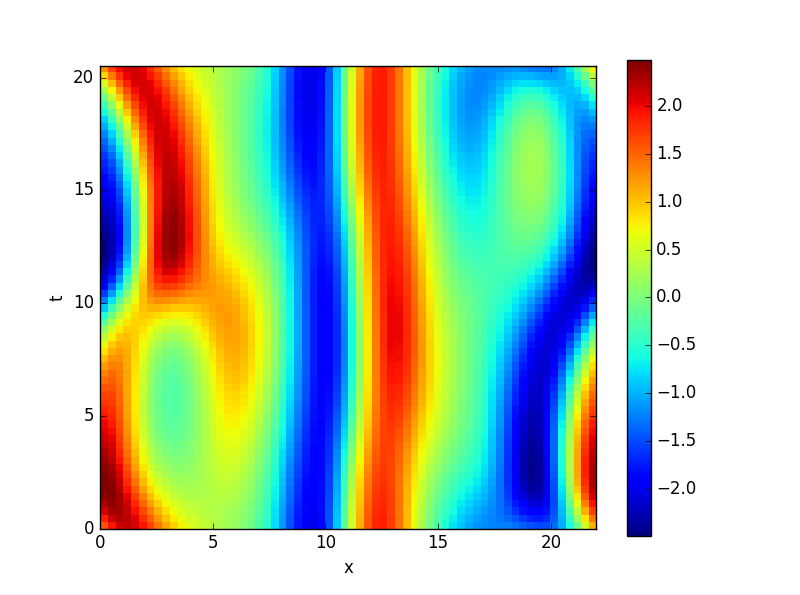
\includegraphics[width=\textwidth,height=.32\textheight]{MNGvndspaceinit1}
\end{minipage}
\begin{minipage}[height=.32\textheight]{.45\textwidth}
\centering \small{\texttt{(b)}}
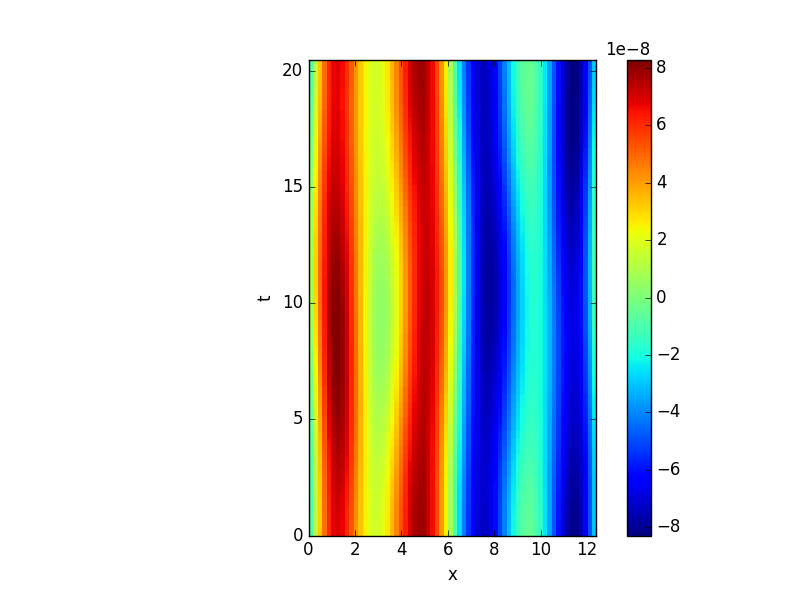
\includegraphics[width=\textwidth,height=.32\textheight]{MNGvndspacefinal1}
\end{minipage}
\caption{ \label{fig:MNGvndspace1}
(a) Initial condition of the 16-by-16 space-by-time discretization of \PPO{10.2} ($L=22$) for spatial
variational {\descent} of the \KSe\
(b) Resulting spatiotemporal \po\ (perhaps badly converged temporal equilibrium), with
final spatial extent of $L = 19.9324743429$
}
\end{figure}



\MNGpost{2017-05-22}{:
Spent the day debugging the spatial {\descent} code, found a negative sign error in the expression for
matrices governing Fourier transforms, converted from taking real(cosine and sine) fft's in one variable (time) to complex fft's
as I was having some trouble reproducing the time derivative term otherwise. Took a while to figure out what was wrong until
I looked at matrix-product results piece by piece and compared to expected results in MATLAB. Rewrote how matrices (derivative
operators) are formulated in terms of the Fourier transform operators. Also found a peculiarity when it came to the accuracy
of matrix multiplcation depending on the order in which the matrices were multiplied...haven't figured that one out yet but nonetheless
I corrected it.

I believe I got it working finally, however, the results so far aren't as
interesting as I had dreamed. I finished this at the end of the day so I didn't
get to test it too much, but so far there are two resulting possibilities.
First, with a time periodic initial condition, i.e. one of the periodic orbits
in time of \KS, when allowing for spatial domain changes and changes to the
temporal Fourier coefficients, the solution (only tested one so far) converged
to one of the temporal equilibria of the \KS\ system. This I believe is an
indication that my code is indeed working, even though this was usually a sign
of numerical issues when searching for periodic orbits in time using the
variational methods, (i.e. the only way to reduce the cost functional
$\mathcal{F}^2 = \lambda v - \tilde{v}$ is to send $v$ and $\tilde{v}$ to $0$.
The reason I believe this is still valid is because the spatial derivatives of
the equilibrium state found are nonzero; i.e. one of the "spatial periodic
orbits" I have found is indeed the temporal equilibrium of the system.

When using a coarse discretization of 16-by-16 space-by-time points
the spatial domain size that the solution settled to was $L=19.9324743429$, with the
value of cost functional being within machine precision of $0$.

When the spatial discretization was doubled, i.e. a 32-by-16 space-by-time
grid, the resulting domain size was $23.7360639824$.

Likewise, when using a 16-by-32 space-by-time discretization, the resulting domain size was $L=19.9398768032$, which indicates that the
domain size of the converged solution is highly dependent on the (spatial)discretization being using.

The second possibility is a convergence to a zero domain size solution, which in my variational method for time usually indicated an equilibrium of
the system. I.e. the two possibilities were either an equilibrium in time (but still a periodic orbit in space), or a spatial equilibrium.
}


\MNGpost{2017-05-24}{:
\begin{description}
\item[spatial variational]
After more investigation it turns out that the spatial variational code is indeed not working yet. Tried to put
resulting orbits into time integrator in order to reproduce the result and got an unmatching solution.
\reffig{fig:MNGvndspace2} is my
newest "results". It uses a \RPO{16.31} of the \KSe\ as the initial condition. I think I was deceived by how nice it looks
I suppose...couldn't find any errors today that could enable reproduction via time integration.

As an additional test I put the solutions into Burak's symmetry reduced time integrator to verify whether
the "solution" in \reffig{fig:MNGvndspace2} was a \rpo\ but alas there was no luck; there is some other error
that I haven't been able to identify as of yet.

Found another negative sign error, updating \reffig{fig:MNGvndspace1}.

\item[torus code]
Applied changes based on implementation from spatial variational method to my torus finding code but it seems
I jumped the gun as I cannot reproduce any orbits found by spatial {\descent} via time integration.

\end{description}
}

\begin{figure}[ht]
\begin{minipage}[height=.32\textheight]{.45\textwidth}
\centering \small{\texttt{(a)}}
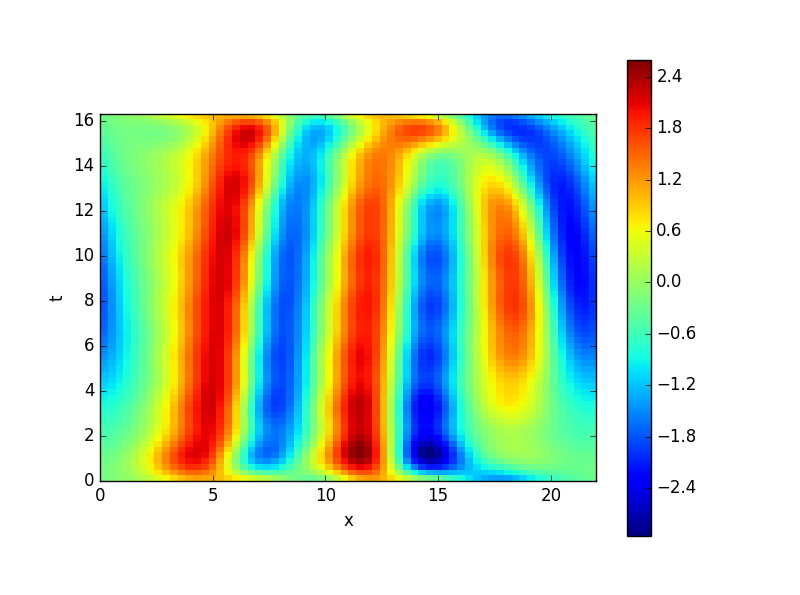
\includegraphics[width=\textwidth,height=.32\textheight]{MNGvndspaceinit2}
\end{minipage}
\begin{minipage}[height=.32\textheight]{.45\textwidth}
\centering \small{\texttt{(b)}}
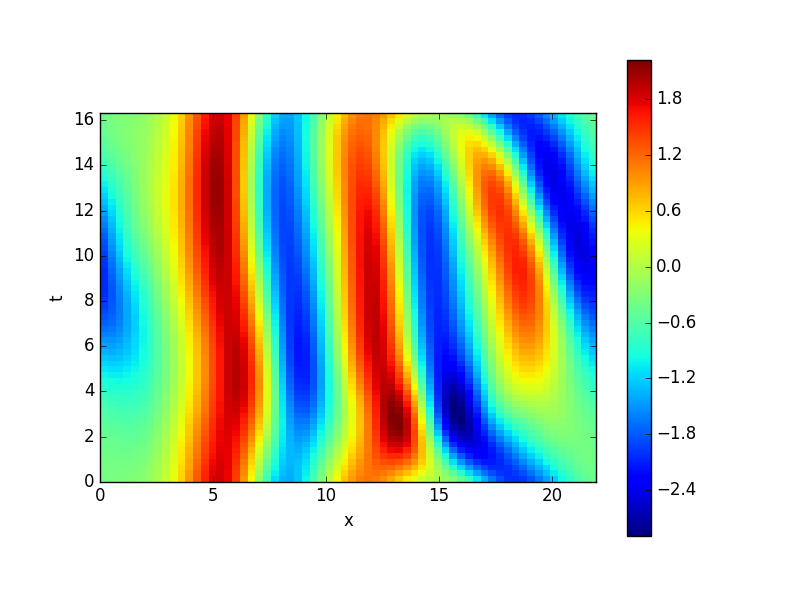
\includegraphics[width=\textwidth,height=.32\textheight]{MNGvndspacefinal2}
\end{minipage}
\caption{ \label{fig:MNGvndspace2}
(a) Initial condition of the 16-by-16 space-by-time discretization of \RPO{16.31} ($L=22$) for spatial
variational {\descent} of the \KSe\ (b)Resulting "spatial periodic orbit" (temporal equilibrium), with
final spatial extent of $L = 21.9394614064$
}
\end{figure}
\begin{figure}[ht]
\begin{minipage}[height=.32\textheight]{.45\textwidth}
\centering \small{\texttt{(a)}}
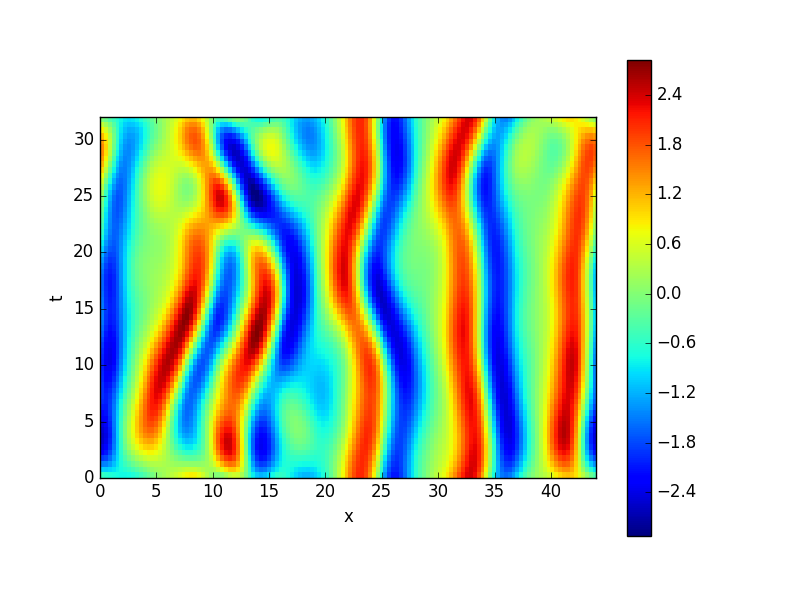
\includegraphics[width=\textwidth,height=.32\textheight]{MNGvndspaceinit3}
\end{minipage}
\begin{minipage}[height=.32\textheight]{.45\textwidth}
\centering \small{\texttt{(b)}}
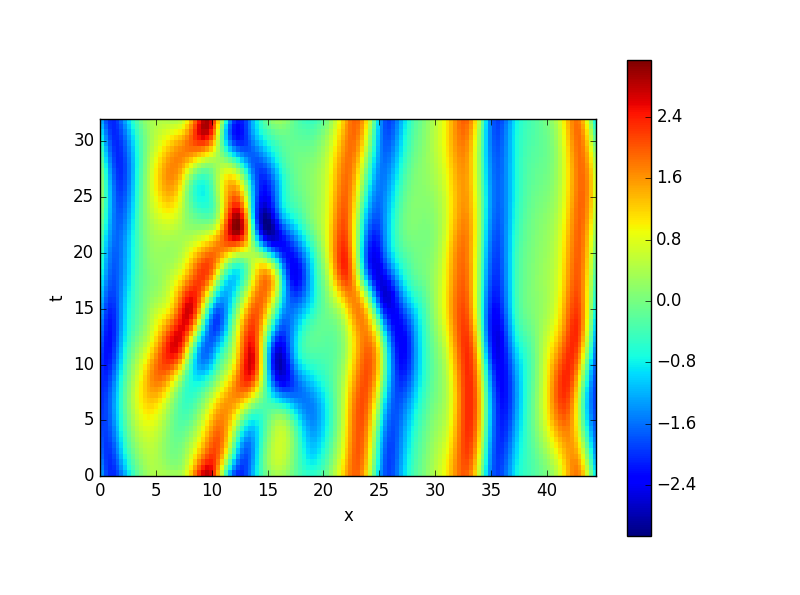
\includegraphics[width=\textwidth,height=.32\textheight]{MNGvndspacefinal3}
\end{minipage}
\caption{ \label{fig:MNGvndspace3}
(a) Initial condition of the 32-by-16 space-by-time discretization of a piece
of an ergodic trajectory that has been deformed to be periodic in time. $L=44$.
(b) Resulting spatiotemporal \po, with
final spatial extent of $L = 44.3937151766$.
}
\end{figure}

\MNGpost{2016-05-27}{:
\begin{description}
\item[updated figures]
updated \reffig{fig:MNGvndspace2}, \reffig{fig:MNGvndspace1}, and uploaded \reffig{fig:MNGvndspace3} to display
current results.

\item[spatial variational]
Found some errors, corrected some bugs, and made some changes that I believe improve my codes. Included a constraint to the variational
equations that constrains the sum of the zeroth temporal modes to be 0. This was done after noticing that
the sum of the zeroth temporal modes over the spatial extent of the loop were within machine precision of 0; I don't
really know what it is a manifestation of just yet but I wouldn't be surprised if this is how the galilean invariance
presents itself in the spatial system.

Still haven't been able to reproduce results from \reffig{fig:MNGvndspace2}, \reffig{fig:MNGvndspace1},\reffig{fig:MNGvndspace3}
via time integration but I also haven't been able to figure out how to use Burak's symmetry reduced integrator appropriately despite
my best efforts.

\item[Floquet vectors]
Arnoldi iterations are complete, starting analysis after checking principal angle codes and automating it.
Preliminary calculations from a single orbit are giving me weird results, in fact, the exact opposite of what
I would expect.
\end{description}
}


\begin{figure}[ht]
\begin{minipage}[height=.32\textheight]{.45\textwidth}
\centering \small{\texttt{(a)}}
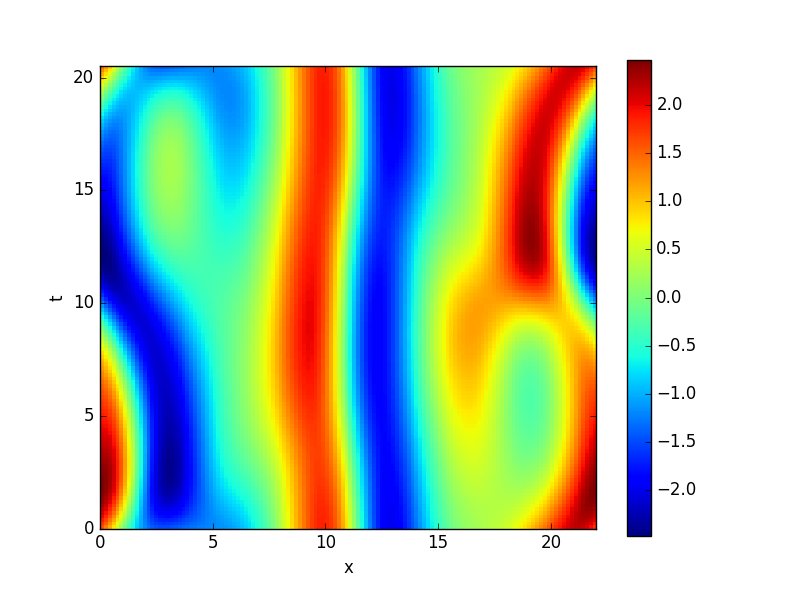
\includegraphics[width=\textwidth,height=.32\textheight]{MNGspacetimeinit1}
\end{minipage}
\begin{minipage}[height=.32\textheight]{.45\textwidth}
\centering \small{\texttt{(b)}}
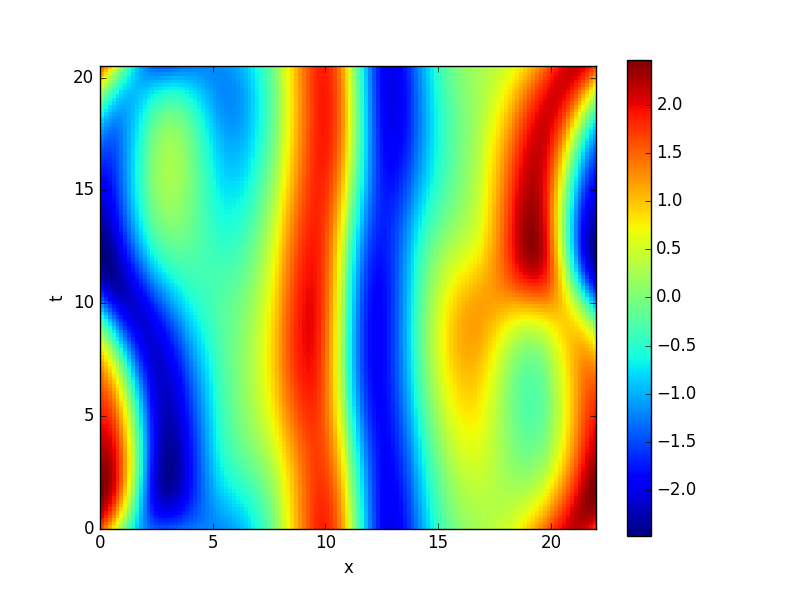
\includegraphics[width=\textwidth,height=.32\textheight]{MNGspacetimefinal1}
\end{minipage}
\caption{ \label{fig:MNGspacetime11}
(a) Initial condition of the 32-by-32 space-by-time discretization of \PPO{10.2}:
$(L_0,\period{0}) = (L_0, 2\period{p_0})= (22,20.5057459345)$.
(b) Resulting spatiotemporal fixed point
$(L_p,2\period{p}) =  (22.0000104401, 20.5057499188)$
}
\end{figure}


\MNGpost{2017-05-30}{:
Found some bugs and errors in the spatiotemporal fixed point code. With spatiotemporal initial conditions generated by time integrating \PPO{10.2}, \PPO{14.3} with initial residuals of $\approx 0.0013$ and $\approx 0.000226$ respectively, the residual is reduced to $\approx 10^{-9}$. Including figures. Still trying to figure out how to set up
the mapping for relative periodic solutions, i.e. how to include a parameter that controls the drift associated with the group orbit.

Still can't figure out why the spatial variational converges to within
machine precision but cannot reproduce results via time-integration.
}

\begin{figure}
\begin{minipage}[height=.32\textheight]{.45\textwidth}
\centering \small{\texttt{(a)}}
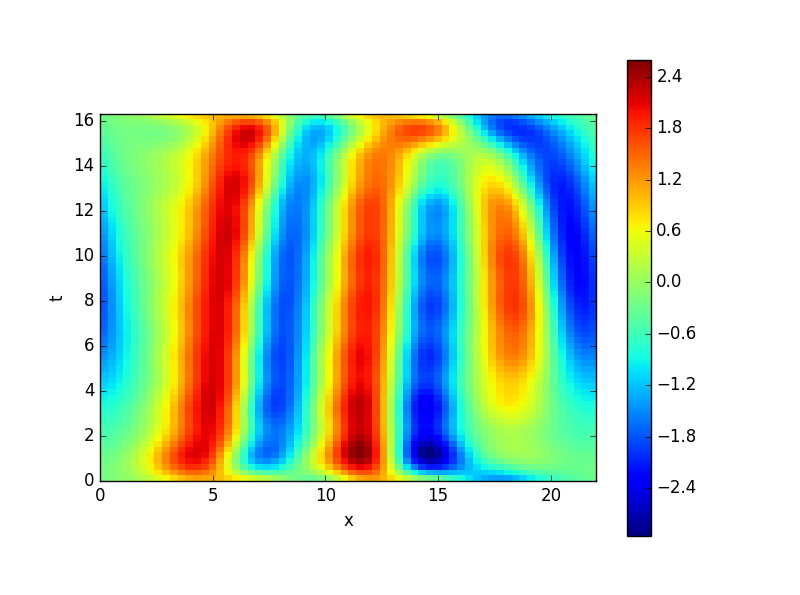
\includegraphics[width=\textwidth,height=.32\textheight]{MNGvndspaceinit2}
\end{minipage}
\\
\begin{minipage}[height=.32\textheight]{.45\textwidth}
\centering \small{\texttt{(b)}}
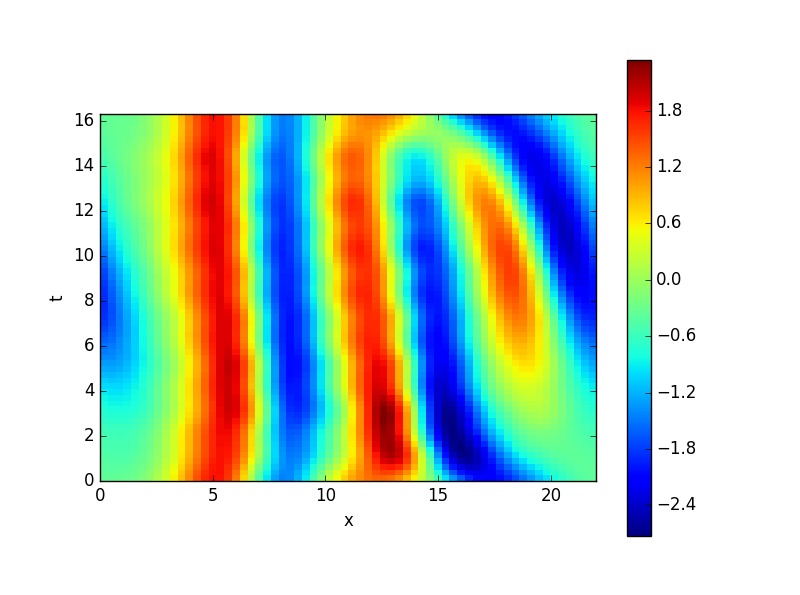
\includegraphics[width=\textwidth,height=.32\textheight]{MNGvndtimefinal2}
\end{minipage}
\begin{minipage}[height=.32\textheight]{.45\textwidth}
\centering \small{\texttt{(c)}}
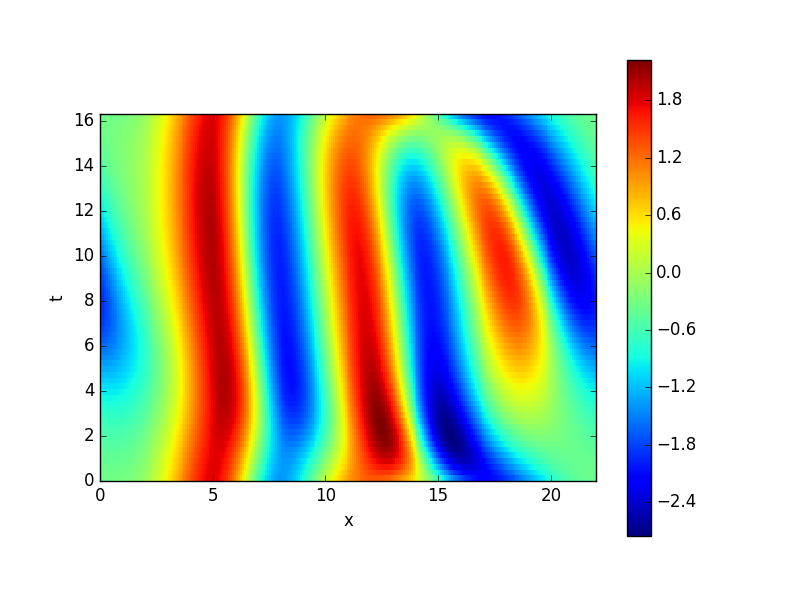
\includegraphics[width=\textwidth,height=.32\textheight]{MNGvndspacefinal2L}
\end{minipage}
\caption{ \label{fig:MNGspaceandtime1}
(a) Initial condition of the 16-by-16 space-by-time discretization of
\RPO{16.31}. $L_0 = 22$.
(b) Resulting periodic orbit after variational {\descent} in time $L =
22, T = 15.7444884386$,
(c) resulting periodic orbit after variational {\descent} in space.
%%%lost the number for final spatial size will need to run code again.
}
\end{figure}

\MNGpost{2017-06-06}{:
\begin{description}
\item[vnd time part two]
As a means of cross-checking results I wrote variational {\descent} code for time, debugged, and got it working. It follows the "direct-matrix" approach
that I have been finding useful.
The velocity equation takes the form
\beq \label{e-MNGkstimeDM}
v = Q_1 \cdot \Fu - Q_2 \cdot F \cdot ((F^{-1}\Fu) \star (F^{-1}\Fu))
\eeq
and the stability matrix is therefore
\beq
A = Q_1 - 2 * Q_2 * \cdot F \cdot diag(F^{-1}\Fu) \cdot F^{-1}
\eeq

I am hoping to use this as a launchpad for other tests for the spatiotemporal fixed point code.

\item[principal angles of Floquet subspaces]
Finished automating code that produces angles between linear subspaces of Floquet vectors. It is running as I type this
and I am hoping that it will be finished by tomorrow morning.

\item[misc]
\reffig{fig:MNGspaceandtime1} is a comparison between resulting orbits from both space and time variational {\descent}.
The general structure of the resulting orbit is preserved even though the periods are quite different. At first I believed that
these were supporting evidence that something is going right but now I am confused. The spatial domain resulting from the \emph{spatial}
{\descent} is largely unchanged, meaning that the orbit that results should be a unique solution with a unique period; but the \emph{time}
variational {\descent} changes the period somewhat drastically, and because the spatial domain size is fixed this might mean that I am
finding the same solution but this is contradictory because the periods are so different. Also good evidence that there is something wrong is that
the \emph{time} {\descent} is taking a \rpo\ initial condition and seemingly changing it into a periodic orbit? I don't know what
to think of it but I am glad that I rewrote the time {\descent} code as it'll be a good stepping stone into whether or not I need to rewrite the equations
in a symmetry reduced form in order to find {\rpo}s or not. I think that's where I'm headed at least.
\end{description}
}

\MNGpost{2017-06-08}{:
\item[torus code and symmetry reduction]
After more debugging and anecdotal evidence from preliminary results of the spatiotemporal fixed point code
I've decided that I should implement a symmetry reduced form of the fixed point finder because it seems to only
work for {\ppo}s and I think this if anything a good practice to implement symmetry reduction.

I debated with myself over how I should implement this; the main two
methods that waffled between were 1. introducing a parameter that governs
the symmetry operation of the \SOn{2} symmetry that would be allowed to
change and or be corrected as the Newton's method implementation runs its
course, or, 2. formulate a ``direct-matrix"\rf{Chu09} for the symmetry
reduced equations as to treat \rpo\ as an invariant 1-torus. I elected for
option two, as I am sort of confused as to how I would implement the
parameter from option one in a spatiotemporal setting as opposed to a
setting where the action of time is still in the setting of a
one-parameter flow.

That being said, and taking much from Chaosbook and \refref{BudCvi14}, this is how I am trying to implement
a symmetry reduced version of my current spatiotemporal code.

Firstly, we must generate symmetry reduced spatiotemporal initial conditions, this, plainly, is done by
using a symmetry reduced time integrator such as Burak's \texttt{ksETDRK4red.m} to generate a spatiotemporal
discretization that will be used for the hunt.

Next, I rewrite the direct-matrix equations in a symmetry reduced form. I find it easiest to first
look at the symmetry reduced velocity equations for \KSe\ and then figure out what is necessary to take
the leap into turning them into a spatiotemporal mapping such as \refeq{e-FksSpattemp}.

Taking equations (8),(9) from \refref{BudCvi14}, the symmetry reduced flow takes the form
\bea
    \hat{v}(\hat{a}) &=&
                v(\hat{a}) - \dot{\theta}(\hat{a})t(\hat{a}) \,, \quad
    \dot{\theta}(\hat{a}) =
                \frac{\langle v(\hat{a}) | t'(\hat{a}) \rangle}{\langle t(\hat{a}) | t'(\hat{a}) \rangle} t(\hat{a})    \,, \quad
    \label{e-symred}
\eea

Now, in order to put this symmetry reduced flow
into a spatiotemporal setting, where the entire orbit is then treated as a vector in the domain the spatiotemporal mapping,
we must make note that for the $N-by-M$ discretizations that we are going to use in the fixed point finder
we need to expand these formulae to account for the fact that we need $M$ copies of the template vector $t(\hat{a})$ for every
point in time; likewise in order to evaluate the group tangent of at for the $2NM$
dimensional vector (2 because of Fourier)
we need to take a Kronecker product between the identity and the \SOn{2} generator in order to have a
$[2NM\!\times\!by-2NM]$ matrix that
will produce the correct group tangent after multiplication with the spatiotemporal vector.

Now once we have all of these things in place we can produce an equation similar to \refeq{e-FksSpattempMat} for the
symmetry reduced flow. Substituting $v$ from \refeq{e-MNGkstimeDM},
(the transparency) the symmetry reduced flow can be written as
\beq
\hat{v}(\hat{a})= \frac{\partial a}{\partial \tau} = f(a),
\eeq
where $\tau$ is the in-slice time.

Then applying an operator $F_t$ that takes the temporal Fourier transform around the orbit, and rewriting the time-derivative
by exploiting the Fourier transform we are left with
\beq
W_{\tau}*\hat{u} - F_{\tau} \cdot f(\hat{a}) = 0
\eeq
Now, for the record, I write the equation in its complete
direct-matrix, symmetry reduced form.
\bea
0 &=&
W_{\tau}*\hat{u}
- F_t ( Q_1 \cdot \Fu - Q_2 \cdot F \cdot ((F^{-1}\Fu) \star (F^{-1}\Fu))
    \ceq
- \frac{\langle Q_1 \cdot \Fu - Q_2 \cdot F \cdot ((F^{-1}\Fu) \star (F^{-1}\Fu)) | t'(\hat{a}) \rangle}
       {\langle t(\hat{a}) | t'(\hat{a}) \rangle} t(\hat{a}))
\eea
where $\Fu$ is now the vector quantity that completely describes the spatiotemporal symmetry reduced orbit in question.

Note: the definitions of the operators before taking Kronecker products are from \refeq{e-MNGwoperator}, \refeq{e-MNGq1operator}, \refeq{e-MNGq2operator}.
}

\MNGpost{2017-06-08}{:
\begin{description}
\item[symmetry reduction implementation]
Spent the second half of my adventure writing components to reduce spatial translational symmetry in the
codes I wrote earlier this week for {\descent} in time for the full-{\statesp}.
I should be able to plug this right into the spatiotemporal fixed point code
once I get it working and I feel that this is a good test-bed. This essentially covers what I wrote earlier
this morning.

I can't seem to figure out why currently but the resulting symmetry reduced velocity isn't of the proper
form i.e. it has a component out of the first Fourier mode slice still. I wasn't able to pin down the error
but I'm hopeful I'll figure it out by tomorrow.

\item[floquet]
small error in automation procedure means I have to run angle producing code again.
graphs of angle distributions for each subspace by tomorrow most likely.
\end{description}
}

\MNGpost{2017-06-09}{:
Finished producing preliminary angle data and figures and codes that allow for plotting.

Went over preliminary data from angle figures with Predrag.
\begin{enumerate}
  \item
Taking a cue from the Lorenz system (see the series of ChaosBook examples
on Lorenz):
\\
the Lorenz invariant subspace --the $z$ axis-- has a very simple
dynamics, with the single \eqv\ the attracting \eqv\ at the origin.
However, if its stability is computed in the full 3D \statesp\ (as it
always must be), the invariant subspace turns out to be unstable, with a
strongly repelling full \statesp\ Floquet eigenvector that makes the
subspace isolated from the full \statesp; you can exit it with any small
generic perturbation, but there is no probability of coming back -
indeed, all the ergodic density is concentrated on Lorenz ears, one never
approaches the $z$ axis.
\\
Conclusion: the Lorenz chaotic dynamics, is far away from,
and nothing like the invariant subspace dynamics.

  \item
Taking a cue from the \KS\ system:
\\
The dimension of the \KS\ (antisymmetric) invariant subspace $\bbU^+$ (imaginary
parts of Fourier modes only) is half of the dimension of the full \statesp.
To approach it, one would need half of the coordinates to tend to zero.
That is possible if the invariant subspace had all eigenvectors that point
out of it stable, but that is not the situation for chaotic dynamics
cases studied. To approach the invariant subspace, 30 out of 60 (let's say)
coordinates would have to be zero or close to it - very unlikely...
  \item
The invariant subspace $\bbU^+$ is the subspace of antisymmetric functions;
functions that repeat themselves twice over domain $L$ (up to a
reflection). In other words, the size of the domain is $L/2$. As we
expect the number of physical degrees of freedom to scale linearly with
$L$, the physical dimension of the subspace is half of the full \statesp;
it is much less chaotic than the full \statesp.
\\
Conclusion: the \KS\ chaotic dynamics, is far away from,
and nothing like the invariant subspace dynamics.
So why in so many problems (\KS, \cGL, Navier-Stokes ...) people study dynamics
in invariant subspaces. For convenience only; they are easier (almost no one
knows how to reduced continuous symmetries), they have {\po}s rather than {\rpo}s
embedded in the ergodic sea, etc. That's what we are doing with Gibson's
{\po}s data set; unphysical, but available.
  \item
other periodic
orbits on the attractor in the full {\statesp}. I.e. Make sure that
Floquet vectors themselves are in the invariant subspace, otherwise
will not really get good information as once one leaves an invariant
subspace there is no
  \item
Only want Floquet vectors that lie in invariant subspace, as taking cues
from Lorenz system, the invariant system is isolated from other periodic
orbits on the attractor in the full {\statesp}. I.e. Make sure that
Floquet vectors themselves are in the invariant subspace, otherwise
will not really get good information as once one leaves an invariant
subspace there is no

  \item
Making sure to use only prime period due to stability and that information isn't being repeated.
Might have to redo arnoldi iterations such that perturbations are contained within the same invariant
subspace as the solution. If not, I should definitely check if Floquet vectors of solutions of
the invariant subspace lie in the invariant subspace to get good angle infromation. I can
test this by whether or not the Floquet vector is invariant after application of discrete symmetry
operation.

  \item
For Floquet multipliers that come in a complex conjugate pairs I need to treat
the plane spanned by the two vectors as a single geometrical object when computing the
principal angles arising from subspaces.

  \item
To harken back to invariant subspaces, inertial manifold described by invariant solutions
on the attractor and not necessarily solutions that lie in invariant subspaces due to isolation, i.e.
the solutions are "far-away" when taken in the context of the dynamics.
I.e. need orbits that are part of the attractor; it is believed that solutions in
channelflow database indeed are taken from the attractor due to
finding initial conditions for Newton-Krylov search from ergodic trajectory and recurrence plots.

  \item
Need to go over an document how the statistics were produced. how the angles were produced.

  \item
Whether one must constrain perturbations to invariant subspace in order to guarantee the Floquet vectors
all remain in the invariant subspace. (small number of orbits that I would need to redo arnoldi iteration for in
this case.

\end{enumerate}

}

\MNGpost{2017-06-13}{:
\begin{description}
\item[symmetry reducing]
Still rewriting code to be able to find {\rpo}s in hope that it will improve the spatiotemporal
fixed point code. I thought it wasn't working because there were problems
with how I implemented the combination of template point of the slice and symmetry reduced velocity
equations but I forgot I needed to also change the stability matrix definition to pertain to
symmetry reduced velocity equations.

\item[floquet vectors]
Trying to figure out the best implementation for what I discussed with PC on Friday. I think I'll have to
import the values of the Floquet multipliers via the text file generated by arnoldi iteration, and for
each $n$th subspace calculation, check if the imaginary part of the Floquet multiplier is zero or not,
and then either calculate the angle of the $n$th subspace or skip to $n+1$ as to include the plane
spanned by the two Floquet vectors instead of splitting them into two different complementary subspaces.
\end{description}
}

\MNGpost{2017-06-13}{:
\begin{description}
\item[starting over arnoldi iterations]
J. Gibson, PC and I realized that in my calculation neither the orbits
nor the Floquet vectors were constrained to the flow-invariant subspace.
The {\po}s stay (up to small numerical errors) in the subspace, but one
should not include the Floquet vectors that point into the full \statesp;
the dynamics within the invariant subspace has little to do with the
dynamics on the full \statesp\ chaotic attractor, an object that is
distant from the invariant subspace (see the {\bf 2017-06-09} discussion
above) and therefore the principal angles for these Floquet vectors
describe neither the subspace inertial manifold nor the full \statesp\
inertial manifold.

In other words the procedure that I need to enact as soon as possible includes

\begin{enumerate}
\item Get \emph{additional} periodic solutions of the Hamilton, Kim, Waleffe cell from J.Gibson mentioned in hangouts meeting.
\item Make sure that the solutions are highly accurate by running them through Newton-Krylov code.
\item Confirm with J. Gibson that I am handling the symmetry operations correctly as to not do this again.
\item Integrate in time while constrained to invariant subspace.
\item Arnoldi iterations with constraint on the velocity field and the perturbations to invariant subspace
to get Floquet vectors that also lie in invariant subspace.
\item Check to see if Floquet vectors are invariant under symmetry operation (checks and balances).
\item Principal angle calculation with geometric properties (no splitting between complex conjugate pairs)
taken into consideration
\item Check to see if trajectories shadowing {\po}s lie in the span of the Floquet vectors
\item Produce plots of principal angles between complementary subspaces of Floquet vectors.
\end{enumerate}

Most of these things are automated already, but the arnoldi iterations and Newton-Krylov codes will take time
to run. I think I should elect for smaller discretizations by not saving as many time-integrated points,
as it would take less time,
but have some thoughts and comments about the discretizations.

\color{red}
I might want to take into consideration the varying importance of different orbits.
The premise for this idea is that shorter orbits have a more pronounced effect on the dynamics. In this vein,
weighing the shorter periodic orbits higher, through a larger discretization,
might be more beneficial in elucidating the geometric structure of the inertial manifold.

On the other hand, if the goal is to capture the geometrical information without redundant information,
a smaller discretization
might be favorable. I am using the $L_2$ distance between the initial condition
and the successive points of the orbit's discretization to give me an idea of how close the points are in the invariant
subspace and perhaps use this as the crudest of measure to avoid repetition.
\color{black}
Currently running the Newton-Krylov convergence in an automated fashion on the previous orbits that I had. Just to make
sure that the information we are getting is as accurate as possible, considering I have to redo the entire process anyway.

\item[symmetry reducing]
Made some changes for the variational {\descent} routine to take keyword arguments such that
one can choose between the symmetry reduced routine for trying to find {\rpo}s and the full {\statesp} routine for {\ppo}s.

Added definition of symmetry reduced stability matrix following equation 13.24 from Chaosbook,
edited some other changes to quantities involved in symmetry reduction to fit with taking real valued
FFTs.
Preliminary tests still show bad results. Need to do more debugging and testing tomorrow.
\end{description}
}

\MNGpost{2017-06-15}{:
\begin{description}
\item[floquet]
After finding some errors in filenames and symmetry files I have the solutions from
John's database rerun in the Newton-Krylov solver.

Also produced the discretizations through DNS for the orbits. I am opting to have
32 points per orbit. This is a compromise to have fewer points per orbit but as the periods
differ by up to a factor of 6 I feel that this still weighs the shorter periodic orbits more
as there are more sample points per unit of DNS time. Again, the main motivation is time, if I could
compute in infinitesimal time I would like to have more points per orbit; secondly, it's a compromise
between treating different periodic orbits the same or differently.

By using a smaller number of arnoldi iterations and number of points on each orbit it will
dramatically speed up the process (not to mention not making mistakes).

Arnoldi iterations are currently running such that the floquet vectors are constrained to the same
invariant subspace as the solutions that they are being produced by; I'm not sure if I should
run four different calculations for the possible antisymmetry and symmetry pairs or if I need
to just include all of the symmetry generators for all possibilities in one run.

In more detail, the complete symmetry group of solutions that I am
working with is described by the ascii representation of symmetry group
elements

\bea
e &=& 1, \,1, \,1, \,1, \,0, \,0
         \continue
s_{xyz} t_z &=& 1, \, -1, \, -1, \,-1, \,0, \,0.5,
        \continue
s_z t_x &=& 1, \,1, \,1, \,-1, \,0.5, \,0
          \continue
s_{yz} t_{xz} &=& 1, \,-1, \,-1, \,1, \,0.5, \,0.5
\eea
where, the symbols follow the following order, and have the respective
effects on solutions
\bea
&&(c, s_x, s_y, s_z, a_x, a_z)[u,v,w](x,y,z)
\continue
    &&\quad\to
\ceq\qquad
    c [s_x u, s_y v, s_z w](s_x x + a_x L_x, s_y y, s_z z + a_z L_z)
\nnu
\eea
J. Gibson seems to agree that I have the symmetry files in order for
constraining the periodic orbits to this symmetry subspace described above. Now all I am
wondering if it is only this symmetry subspace that is of interest
to constrain Floquet vectors to, or if the "antisymmetry" combinations
denoted by a value of $c=-1$ for combinations of two of the symmetry group elements
(i.e. given the above set, the "antisymmetries" would be given by maintaining the same
symmetry group but including negative signs on the following pairs, leaving the other
elements unchanged.\\
 $(-s_z t_x, -s_{yz} t_{xz}), (-s_{xyz} t_z, -s_{yz} t_{xz}),(-s_{xyz} t_z, -s_z t_x)$
 needs to also be taken into consideration.

\item[symmetry reduction]
Still can't get the routine to work for finding {\rpo}s of the time system. The initial
residual is a little high than what I would expect so I think I need to go over the definition
of symmetry reduced velocity again. A rework might be in order for all of the symmetry reduction
parts but only time will tell based on work put in tomorrow, now that I believe I have all of the
arnoldi iterations running for my other project I think (as long as I got the symmetry groups for
the floquet vectors correct then I can focus solely on this again).


\end{description}
}

\MNGpost{2017-06-16}{:
\begin{description}
\item[floquet]
I was worried about some preliminary results from arnoldi iterations so I stopped them and try to think about
the problem a little bit more. It seems that by constraining the floquet vectors to the same invariant
subspace as the solution I was losing out on information and needed to also calculate the floquet vectors
that lie in the "antisymmetry" subspaces as well. These subspaces are categorized by a negative sign
assigned to one of the generators.

What tipped me off was that during the current iterations there is a lack of the three marginal floquet
vectors, and from as far as I can tell by restricting to the same invariant subspace as the solution,
the arnoldi iteration only includes one of the three.

By writing out the multiplication table of the group I am attempting to solve this problem by changing
the list of generators from
\bea
s_{xyz} t_z &=& 1, \, -1, \, -1, \,-1, \,0, \,0.5,
        \continue
s_z t_x &=& 1, \,1, \,1, \,-1, \,0.5, \,0
\eea

to the following:
\bea
s_{xyz} t_z &=& 1, \, -1, \, -1, \,-1, \,0, \,0.5,
        \continue
s_z t_x &=& 1, \,1, \,1, \,-1, \,0.5, \,0
          \continue
-1*s_{yz} t_{xz} &=& -1, \,-1, \,-1, \,1, \,0.5, \,0.5
\eea

where as before, the lists of numbers follow the notation ${c,s_x,s_y,s_z,t_x,t_z}$ where $s$ stands for
shift-reflect and $t$ stands for shift-rotate in the appropriate variable as denoted by the subscript.

This seems to be incorrect however, as all of the floquet vectors belonging to this space are stable.

\item[floquet after PC meeting]
After talking to PC about the concerns noted above it it appears that I was computing the iterations correctly,
and that all my worries were for nought. This is good in a way as the communication between us gave us a better
mutual understanding of what I am actually computing; however, it also means that I wasted half of my day chasing
ghosts. I think it was for the best as it gave me a better understanding of the problem and will prevent confusion
in the future however.

\item[symmetry reduced variational method]
Finding some better numerical results with the alternate definitions for
\refeq{e-symred} which are, ($x_i$ implying real part of $i$th Fourier mode,
$y_i$ is the imaginary part, where $i = 1, ..., N/2-1$

\bea
    \frac{\partial \hat{a}}{\partial \tau} &=&
                \hat{x}_1 v(\hat{a}) - \dot{y}_1(\hat{a}) t(\hat{a}) \,, \quad
    \frac{\partial \theta(\hat{a})}{\partial \tau} = \dot{y}_1(\hat{a})
                   \,, \quad
    \label{e-symred2}
\eea

Currently trying to figure out the correct way of reconciling this new definition with
direct matrix implementation.

I believe that the stability matrix with take the following form,
\beq
\hat{A} = diag(x_1)\cdot A - diag(\dot{y}_1(\hat{a}))\cdot T
\eeq

\end{description}
}

\MNGpost{2017-06-19}{:
\begin{description}
\item[floquet vectors]
Based on the current progress, I estimate that the arnoldi iterations will be done by next
weekend.

I am currently writing some new portions of code that will take in the files storing
the floquet multipliers as to make sure that vectors corresponding to complex conjugate
multipliers are not separated into different subspaces during angle calculations.

I am currently only going to take 32 points per orbit to see if I can get a rough idea
for the angles. If need be I can always procure more points on orbits and do the arnoldi
iterations for the additional points.

\item[symmetry reduction variational method]
Finished implementing the newer version of symmetry reduction variational method
\refeq{e-symred2}.
Still having issues as initial condition for the value of the cost-functional, which
is the best indication I have that I am still somehow messing up the symmetry reduced equations;
the only other contributor could be the approximate loop tangent, which I realized today
should also be symmetry reduced, i.e. it doesn't make sense to compare the in-slice velocity
to an \MNGedit{approximations of element in the full {\statesp} tangent bundle}.

I know it isn't any of the definitions that I would be using for {\ppo}s because, for example,
an initial loop defined on 32 points in space and 128 points in time for \PPO{10.2} starts with an initial
value of the cost functional of $F^2 \approx 10^{-10}$ which is far better than anything that I have
ever had before, and of course as a sign of it's working it reduces the residual to within machine
precision with the correct period.

When I try this type of discretization with \RPO{16.3} I have no luck, and I get the "converging to equilibrium"
problem that usually indicates I have contradictory definitions or something else the matter.
So there must be something else that I am either forgetting or not paying correct attention to.

I did find a bug, however, where in the computation of the cost functional, sometimes the wrong
definition of velocity would be used; this helped reduce the initial cost functional value for
{\rpo}s to order $\approx 10$. I think it might be time to talk to Burak and see if he agrees
with the definitions I'm using as I am running out of ideas.
\end{description}
}

\begin{figure}[ht]
\begin{minipage}[height=.32\textheight]{.45\textwidth}
\centering \small{\texttt{(a)}}
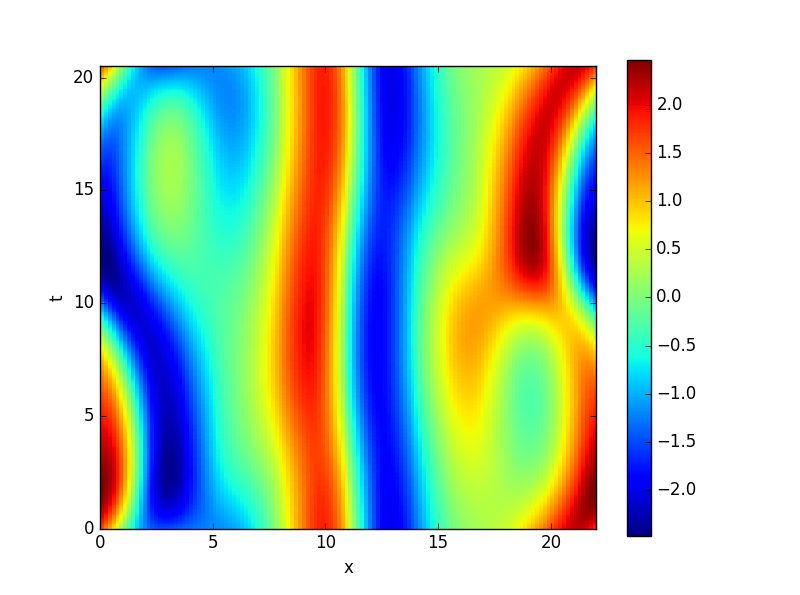
\includegraphics[width=\textwidth,height=.32\textheight]{MNGvndtimefinal1}
\end{minipage}
\begin{minipage}[height=.32\textheight]{.45\textwidth}
\centering \small{\texttt{(b)}}
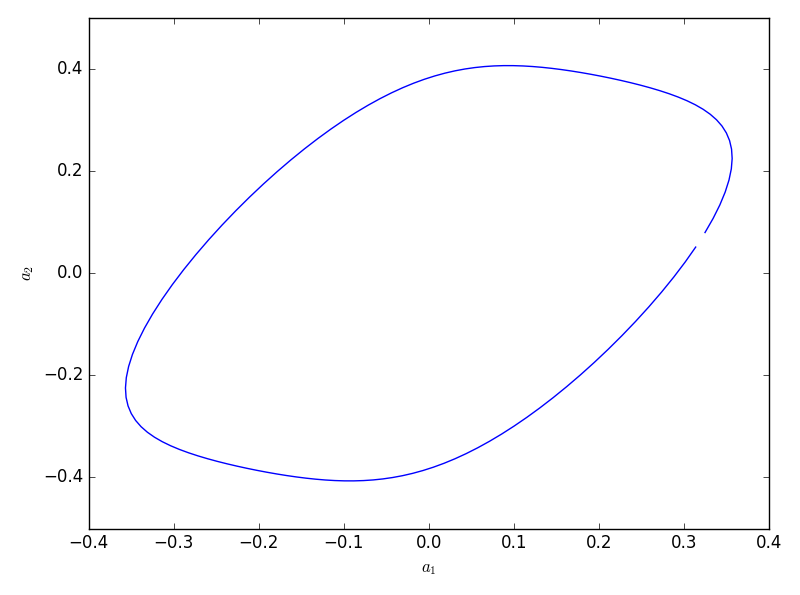
\includegraphics[width=\textwidth,height=.32\textheight]{MNGvndtimeproj1}
\end{minipage}
\caption{ \label{fig:MNGspacetime1}
(a) 32-by-128 space-by-time discretization of \PPO{10.2} resulting from
temporal variational method.
(b) Fourier-mode projection of (a) on the first two real parts of spatial
Fourier coefficients $a_1, a_2$.
}
\end{figure}

\MNGpost{2017-06-20}{:
\begin{description}
\item[symmetry reduced variational]
Including a checklist of possible faults of my symmetry reduced
variational method code, ranked in terms of likeliness. I've already
checked these definitions a number of times but until I can verify with
one-hundred percent certainty that they are correct I will leave them here unmarked. In other words they are possibly the outstanding issues.

\begin{enumerate}
\item function definition of symmetry reduced velocity equation
\item function definition of symmetry reduced stability matrix
\item Whether approximate tangent field operator needs to be symmetry
reduced. (I believe so).
\item Generation of symmetry reduced {\descent} matrix (based on velocity and stability matrix being reduced)
\item Slice template vector
\item Infinitesimal generator of rotations T
\end{enumerate}

Next are the things I know have no problem as they work perfectly with
{\ppo}s.

\begin{enumerate}
\item Operators that produce spatial, temporal derivatives.
\item Operators that perform forwards and backwards Fourier transforms
\item full {\statesp} velocity
\item full {\statesp} stability matrices
\item fictitious time stepping routine
\item Operator that produces full {\statesp} approximation to tangent field.
\end{enumerate}

\item[meeting with burak]
Planning on talking to Burak tomorrow if I can't get the symmetry reduced variational
code to work by tomorrow.

\item[additional figs]
Included the figures of results from full {\statesp} variational method to find \PPO{10.2}
for completeness. These include a two-dimensional Fourier mode projection and the full
spatiotemporal velocity field.


\item[Microextensive chaos of a spatially extended system] Wanted to read
\refref{tajima02} as it was referenced in \refref{XuPaul16} but ran out
of time.

\end{description}
}

\MNGpost{2017-06-23}{:
After being frustrated for a while I finally realized the dumb mistake I have been making
when it comes to symmetry reduction. I have been trying to compute the symmetry reduced
velocity at every point of the discretized symmetry reduced {\rpo}s all at once. This was
the wrong choice because the equations rely on inner products of vectors specific to each point
along the discretization (namely the full \statesp\ velocity and the group tangents at
the slice template point and each time discretization point).

I don't know why I didn't realize this before (I guess I'm learning?) but something clicked
when I noticed that the wrong elements were being set to zero in my previous formulation, in other
words the in-slice symmetry reduced velocity wasn't tangent to the slice.
I tested out the formulae I have been using for a single point along the discretization in time and everything resolved.

In more detail, previously I was using a template point that was the same dimension as the entire discretized
orbit, i.e. for an $N-by-M$ space-by-time discretization of an \rpo\ I was using $M$ copies
of the same template vector expecting it to work but this is fundamentally flawed because
when I use the equations \refeq{e-symred} all this does is mix all of the information of
the orbit together in a jumbled fashion that makes absolutely no sense.

It probably doesn't need to be said, as I have been doing this for about a week but again
I reiterate that I am working on a way of reconciling the formulae with the direct-matrix
implementation that I have been using.

If I can't figure out a way then there is the back-up
plan of performing operations one at a time (as opposed to using
linear operators that act on the entire discretized orbit at once)
by computing the symmetry reduced velocity of each \statesp\ point and each symmetry reduced
stability matrix one by one and then compiling them respectively into the vector, matrix that I need:
A vector containing the in-slice velocities at every point along the orbit and a block
diagonal matrix whose blocks are comprised of in-slice stability matrices evaluated as the
respective point along the orbit.

Before rewriting this portion I am still going through the list of other possible defects.
So far I can verify that the group tangent of the template point and the generator of infinitesimal
rotations is valid. I am getting wrong results for the full {\statesp} velocity as compared
to Burak's MATLAB codes which I can't explain at the moment, considering those definitions
worked fine for {\ppo}s.

All in all tomorrow will hopefully be a good day for my research.
}

\MNGpost{2017-06-27}{:
Found a negative sign compatibility error in Burak's symmetry reduction code
that I was using to produce initial conditions. I believe this goes
back to other MATLAB codes for \KS\ that contained conjugation where
it wasn't correct, similar to compatibility issues I had with
my spatial integration code.

Wrote code that computes the symmetry reduced velocities each temporal
discretization point at a time and likewise for the symmetry reduced
stability matrices.

These two combinations dramatically reduced the initial values for
cost functionals in the variational Newton code, however I am still getting problems with convergence likely due to a small error somewhere,
or some problems with how I am trying to circumvent the issues.

This workaround also rises concerns for how I am going to implement the
symmetry reduction in the spatiotemporal fixed point codes, as I try to
treat the solution to the spatiotemporal fixed point equation as one object, as I believe it should be. That being said I am still trying
to find a way to work with entire orbits instead of this way because it
doesn't feel too intuitive. I am working through another way which
I will write up once I am confident in its accuracy.
}

\MNGpost{2017-06-27}{:
\begin{description}
\item[inertial manifold]
Arnoldi iterations are taking longer than I had remembered. Will probably been done by next weekend.

\item[symmetry reduced variational methods]
After I posted yesterday I almost immediately figured out the issue with the current formulation and why it won't work. It's a matter
of the ordering of the variables; the way I have the code currently written the variables are ordered in a spatiotemporal vector
that cycles through the time first and then space. I.e. if $k$ and $\ell$ were indices that take values from $0, \cdots, N-1$
and $0, \cdots, M-1$ respectively representing the the space and time discretization, for every unit change to $k$, the index
$\ell$ would have cycled through $M$ values.

Now, this isn't important it's just a clerical part of coding but the problem I am now facing is that this specific ordering
is going to make it much harder to finish the symmetry reduction variational code. I've tried to work things out
in a number of ways but they are require some very unintuitive measures that I feel would be best to avoid. So, for now,
I am going to rewrite everything such that the ordering of the \statesp\ vector cycles through spatial indices first, in other
words switching to a different standard.

With this in mind, I believe I have a way to rewrite \refeq{e-symred} such that it will serve my purposes of symmetry reduction.
Like I've said before the problem I had from a lack of practice was that I was trying to symmetry reduce the entire orbit at
once not taking into consideration that the group tangent direction (amongst other things) is a time-dependent quantity.

Here is how I believe I can fix things once I change the ordering of the spatiotemporal vector i.e. the orbit in vector form.
It basically relies on computing $M$ copies of \refeq{e-symred} while keeping all of the information at different times separate.
Starting with,
\bea \nonumber
    \hat{v}(\hat{a}) &=&
                v(\hat{a}) - \dot{\theta}(\hat{a})t(\hat{a}) \,, \quad
    \dot{\theta}(\hat{a}) =
                \frac{\langle v(\hat{a}) | t'(\hat{a}) \rangle}{\langle t(\hat{a}) | t'(\hat{a}) \rangle} t(\hat{a})    \,, \quad
\eea

Let $v$ now be matrix whose rows (instead of columns as to reshape the matrix into a vector properly)
are the full \statesp\ velocity evaluated along the time discretization of a symmetry reduced
\rpo. Likewise, define $\hat{a}$ as a matrix whose rows are the current (in fictitious time) representation of the symmetry
reduced \statesp\ points that comprise the \rpo. Then, we can change the inner product notation to a matrix-vector product notation
by virtue of the group tangent template vector being constant. For example, the velocity will now be concatenated in a matrix
in the following manner.

\beq
v(\hat{a}) \rightarrow \mathbf{V} \equiv [v(\hat{a}(\tau_0)) | v(\hat{a}(\tau_1)) | \cdots | v(\hat{a}(\tau_{M-1})) ]
\eeq

following this notation the equation for evaluating the symmetry reduced velocity at every point along our discretization
will be

\bea \nonumber
    \hat{\mathbf{V}}^T(\hat{a}) &=&
                \mathbf{V}^T(\hat{a}) - \dot{\theta}(\hat{a}) \mathbf{t}^T(\hat{a}) \,, \quad
    \dot{\mathbf{\theta}}(\hat{a}) =
                (\mathbf{V}^T(\hat{a}) \cdot t'(\hat{a})*/ \mathbf{t}^T(\hat{a}) \cdot t'(\hat{a})) \mathbf{t}^T(\hat{a})  \,, \quad
\eea

Now the onto the stability matrix; as opposed to the symmetry reduced velocity where
I can just concatenate vectors into matrix and perform element-wise operations and matrix-vector products, with the stability
matrices I needed to rewrite definitions of all of the matrices involved in the direct-matrix derivation which I am
still in the process of. Some of them are easy, where the effect of the reordering merely results in the opposite order
kronecker product.

Hoping to be testing by tomorrow to settle this once and for all.
Submitting the different version of the functions implemented today in different file for versioning purposes. Will delete
once finished.

\item[chats]
Going to chat with Ravi on Thursday at some undisclosed time and place, probably the office on the fifth floor.

\end{description}
}

\MNGpost{2017-06-29}{:
\begin{description}
\item[symmetry reduction]
Wrote code to produce more general initial conditions for symmetry reduced variational methods.
Alright. I have mostly figured out the issues. I guess I was confused on how to use the in-slice time symmetry reduced
velocity in conjunction with the direct-matrix formulation before. I was attempting to use equations \refeq{e-symred}
in place
of something similar to \refeq{e-symred2} and this was a tragic mistake that took me a week to figure out.

The following are what I believe to be the correct implementation of symmetry reduction for the variational
method when applied to a {\rpo} that has been generated with a symmetry reduced integrator. In other words,
when the initial condition is a spatiotemporal discretization embedded in the slice

{\color{red} With this new formulation the initial value of the cost functional is $F^2 \approx 10^{-8}$ for
a symmetry reduced reproduction of \RPO{16.3}. This
is comparable with an excellent initial condition with all of the correct formulae in previous works.}

The new equation I am using for calculation of the symmetry reduced velocities (w.r.t. in-slice time) in the
direct-matrix formulation is,
\beq \label{e-KSsymDMvel}
\hat{v} = (diag(x_1(t)) \otimes I_{N-2})\cdot v - (diag(\dot{y}_1(t)) \otimes I_{N-2}) \cdot (I_M \otimes T) \cdot \Fu
\eeq

This is relatively simple to explain when using \refeq{e-symred2} as a reference. $diag(a_1(t))$ is a diagonal
matrix that when multiplied with the full \statesp\ velocity vector produces a vector whose entries
are equal to $x_1(t_i)*v(t_i)$ where $x_1$ is the real component of the first Fourier mode. likewise for $diag(\dot{y}_1(t))$
except $\dot{y}_1$ is the velocity of the imaginary component of the first Fourier mode. the $\otimes$ symbol here
denotes a Kronecker product (outer product) whose purpose is to copy the values $x_1$ and $y_1$ as to create a diagonal
matrix whose dimension equals the dimension of the velocity vector $v$. i.e. I need an outer product with a $N-2$ identity
matrix to ensure that I have $N-2$ copies of $x_1$ and $y_1$ so that each of the $N-2$ Fourier modes gets multiplied by
the correct factor.

To simplify the notation and make it more apparent how to derive the stability matrix in direct-matrix notation, I rewrite
$X_1 = diag(x_1(t)) \otimes I_{N-2}$ and $Y_1 = diag(\dot{y}_1(t)) \otimes I_{N-2}$.

The equation for the stability matrix for the entire orbit is therefore.

\beq \label{e-KSsymDMstb}
\frac{\partial \hat{v}}{\partial \Fu} = \hat{A} = X_1 \cdot A - Y_1 \cdot T
\eeq

There is still a small error lurking because despite of the small initial value for the cost functional I still have not
achieved convergence within machine precision.

I believe it might be that I have treated $X_1$ and $Y_1$ as constant matrices as opposed to functions of $\Fu$. This
is the only place that I find room for errors so far.

\item[chats]
Chatted with Ravi about his method of finding heteroclinic connections. Specifically,
we talked about the method of using cotangent inverse as a mapping such that the curve is
reparameterized on a finite interval of real numbers so that Chebyshev functions can be
deployed. Also went over the current issues that he is facing namely the oscillations that
occur around equilibrium (which apparently upon a certain choice can be made to occur in the middle
of the connection). Also went over the adjoint method that he learned from
that Chebyshev functions

\item[arnoldi iterations]
Arnoldi iterations are still going strong.

\end{description}
}

\MNGpost{2017-07-03}{:
Small progress on symmetry reduced variational methods front. With some small changes to how I implemented
\label{e-KSsymDM0}. and playing around
with different discretizations of \RPO{16.3} I was able to get a final result whose value
of the cost functional is $F^2 \approx 10^{-12}$. This is four orders of magnitude of improvement
from the initial value of $F^2 \approx 10^{-8}$ but it's still not good enough.

The new formulations of \refeq{e-KSsymDMvel} and \refeq{e-KSsymDMstb} are written in the following ways, to more
explicitly represent the dependence of the matrices $X$ and $Y$ on the underlying quantities, namely the
orbit vector (vector representing the time discretizations of the spatial Fourier series)
and the full {\statesp} velocity vector.

\beq \label{e-KSsymDMvelnew}
\hat{v} = (X \cdot \Fu) \ast v - (\dot{Y} \cdot v) \ast (I_M \otimes T) \cdot \Fu
\eeq

with this (more) correct direct-matrix velocity equation we can then derive the corresponding stability matrix,
using the rules of calculus described in \refref{Chu09}

\beq \label{e-KSsymDMstbnew}
\frac{\partial \hat{v}}{\partial \Fu} = \hat{A} = diag(v)\cdot X + diag(X \cdot \Fu )\cdot A - diag(T \cdot \Fu)\cdot (Y \cdot A) - diag(Y \cdot v)\cdot T
\eeq


The new formulation helped me find an error in how I was deriving the stability matrix as there was dependence on
both the orbit vector $\Fu$ and velocity vector $v$ in the matrices $X_1$ and $Y_1$ in \refeq{e-KSsymDMstb} that
I was not accounting for.

As I previously mentioned this did help a little bit but it did not completely
solve the problem as I still do not have convergence although I have a really
good initial condition (as evidenced by the initial condition's cost functional
value).

I don't see any more room for errors in the stability matrix definitions, so I
think it might be something more idiosyncratic of {\rpo}s, namely, how the time
discretization using in-slice time might be more unevenly distributed as
opposed to the full \statesp\ dynamical time.
}

\MNGpost{2017-07-06}{:
After trying numerous small modifications to the variational method's system
of equations from \refref{LanThesis} including implementing factors involving
the coordinate involved in defining the in-slice time and other quantities
involving the slice tangents I didn't get any improvements over what I already
had. I still think the problem has to do with the slice time so I went over
the derivation of the equations and I believe I found a correction that can be
made.

The derivation of the system of equations used to find the fictitious time
corrections to the initial guess loop involves substitution of the
partial derivative of the rescaling factor with respect to fictitious time.
The way that this is done is via the definition

\beq
\lambda_n = \frac{\Delta t_n }{\Delta s_n} \, ,
\eeq
where, $s$ is the parameterization variable, here defined with a subscript $n$
to indicate that the parameterization need not be uniform around the initial guess
loop (although this is what I work worth as it makes things much easier to program).
$t$ in this instance stands for the real dynamical time of the orbit.

If we substitute the definition for the in-slice time, this equation takes the form

\beq
\lambda_n = \frac{\Delta \hat(t)_n (x_1)_n }{\Delta s_n}
\eeq

Going through the almost identical derivation for the system of equations there
is one place where I believe they differ. Normally, there is the substitution

\beq
\delta t_n = \frac{\partial \lambda_n}{\partial \tau} \Delta s_n \delta \tau
\eeq

Normally this is easily generalized in order to produce a uniform rescaling of the period
around the orbit,
but if the coordinate $x_1$ is involved I believe that this should take the form

\beq \label{e-inslicevarmeth}
\delta t_n = (\frac{\partial \lambda_n}{\partial \tau}(x_1)_n + \frac{\partial (x_1)_n}{\partial \tau} \lambda_n)\Delta s_n \delta \tau
\eeq

As the in-slice time rescaling is coordinate dependent, this formula seems to beg for a description
of the general equation that has a coordinate dependent rescaling. This is kind of what I have been stuck on
as this is quite different from what I am used to.

For a orbit that is described by $M$ points in time we would need ${\lambda_i}$ where $i = 0, ... , M-1$.

I'm currently working on implementing this into my current code but it's gotten the best of me so far.
}

\MNGpost{2017-7-10}{:
The way I am attempting to solve the problem I am having with in-slice time is as such,
for $M$ discretized points representing an in-slice time description of a {\rpo} I am introducing
$M$ different time rescaling quantities $\lambda_m$. In this way the original variational
method equation changes from
\beq
\begin{bmatrix} D - \lambda diag(A_0, ... , A_{M-1}), & -v \end{bmatrix}
       \left[ \begin{array}{c} \delta \tilde{\conf} \\ \delta \lambda \end{array} \right] =
    \delta \tau \left[ \begin{array}{c} \lambda v - \tilde{v} \end{array} \right],
\eeq
to
\bea
&&\begin{bmatrix} D - diag(\lambda_0 * A_0, ... , \lambda_{M-1} * A_{M-1}), & -diag(v_0, ..., v_{M-1}) \end{bmatrix}  \left[ \begin{array}{c} \delta \tilde{\conf} \\ \delta \lambda_{m}
            \end{array} \right]
\continue
&&=
    \delta \tau \left[ \begin{array}{c} diag(\lambda_m) v - \tilde{v} \end{array} \right],
\eea
In this way the correction mentioned in \refeq{e-inslicevarmeth} is not being resolved but I want to try
to see if more flexibility in the rescaling of in-slice time with respect to fictitious time evolution
is sufficient before getting into an equation I derived; it's also a simpler step whose changes could be
carried over to the full in-slice time description I probably will need.
}

\MNGpost{2017-07-12}{:
Making the single change of a non-uniform parameterization rescaling did not help the variational {\descent} for {\rpo}s so I moved onto the modified formulation \refeq{e-inslicevarmeth} in hopes this would
solve my problem.

It was a little tricky to figure out the best way to implement but I got it running with unfortunately
no better performance than the original symmetry reduced variational {\descent} that I had about a week
ago. It could be my derivation of the modified descent equations is off but I am testing some other avenues
currently. Namely, with a non-uniform parameterization with in-slice time I am testing a non-uniform
finite difference scheme to approximate the loop tangent as opposed to a Fourier description.
I feel the non-uniformity of the discretization is probably something to be avoided but I am testing this
as a last stand.

With a $32\times128$ space-by-time discretization of \RPO{16.3} the initial
cost functional value is still $F^{2} \approx 10^{-8}$ so it has some legs to
move in the right direction, i.e. I am not losing too much accuracy by
switching the numerical method approximating the loop tangent. After some
testing this did not help the convergence either and took much longer.

I'm going to recheck the derivation I went through and see if there's anything
I can change while also taking some of the improvements I have learned and put
them to work on the spatiotemporal fixed point codes.
}

\MNGpost{2017-07-20}{:
%Haven't posted in a while because I was suffering from some type of stomach flu earlier in the week
%trying to catch up for lost time
Wrote some new code for symmetry reduced spatiotemporal fixed point finding; currently
it seems a little strange to me because I only know how to quotient the spatial translation
symmetry in spatial Fourier space as opposed to spatiotemporal (double) Fourier space.

The way that this I am attempting this, are with the equations, in direct-matrix notation:

Using the definition of the reduced velocity in time, \refeq{e-KSsymDMvelnew}, restated here
for reference,
\beq
\hat{v} = (X \cdot \Fu) \ast v - (\dot{Y} \cdot v) \ast (I_M \otimes T) \cdot \Fu,
\eeq
We then find the equivalent spatiotemporal system by Fourier transforming in time by means
of application of $F_t$ linear operator denoting the transform and moving everything to one
side. Here, the $\Fu$ stands for a description of the initial solution that is only Fourier in space.
\beq
W\cdot F_t \cdot \Fu -F_t\cdot((X \cdot \Fu) \ast v - (\dot{Y} \cdot v) \ast (I_M \otimes T) \cdot \Fu) = 0
\eeq
The stability matrix resulting from this symmetry reduced mapping is therefore,

where $\hat{A}$ is in reference to the equation previously defined \refeq{e-KSsymDMstbnew}.

\beq
J = W\cdot F_t - F_t\cdot \hat{A}
\eeq

Even though the changes to the system of equations aren't too complex, the previous incarnation
of the code used pretty different set of orderings and other small nuisances that have made it
a debugging nightmare due to my confusion between other variants of my codes, I realize now that
I shouldn't have prepared different initial conditions for every code I write and should have
made everything complementary so that all initial conditions of \KSe\ could be used in
any variant of the the variational codes (albeit still being split between symmetry reduced
versions or not) as well as the Newton's method codes.

The part that troubled me for a while was how to implement symmetry reduction of the spatial translation
symmetry in a spatiotemporal way as opposed to what I have now. I haven't been able to come
up with anything good yet but it just seems like a little bit of a hack job to reduce
the symmetry before taking things to the spatiotemporal stage. Because I am trying
to find fixed points after symmetry reduction I imagined that this case should be
exactly be like symmetry reduction of a \reqva\ but I haven't found a good way of treating
the equations yet.
}

\MNGpost{2017-07-24}{:
Almost finished with symmetry reduced spatiotemporal fixed point code, all that remains is redefining the
partial derivatives of the spatiotemporal mapping with respect to time and domain size parameters in order
to get corrections to the spatial domain size and period.

Made some changes that make the problem seem more natural, namely, I included some terms such that everything
is in terms of linear operators acting on vectors of spatiotemporal Fourier coefficients as opposed
to a weird mixture I had before. The upside is that everything is defined spatiotemporally, but it might
look a little odd at first glance because there are certain terms which only have one type of Fourier transform operator being applied.

I also elected to change the temporal Fourier transform to a RFFT based description as opposed to a FFT
based description (FFT produces both sides of the spectrum, negative and positive Fourier modes based on index
where RFFT just produces half of the spectrum). I avoided this earlier because it was easier at first but
now that I have some experience this RFFT based description is definitely desired as it minimizes the number
of variables in the system. (It is possible, of course to take a FFT and then keep half of the terms but
this would be hard to implement given my direct-matrix implementation). The problem isn't completely
symmetric in terms of space and time however, as the Galilean invariance eliminates the need to keep
track of the terms corresponding to zeroth and Nyquist $(N/2)$ modes of the spatial spectrum; The easiest
way to describe this is that the discretization in spatiotemporal Fourier space is $N-2 by M$ where $N$
is the spatial discretization and $M$ is the temporal discretization.

With this description the new equation for the spatiotemporal mapping takes a similar form to what I was
implementing the last time I posted, with a few changes.

The mapping now takes the form,
\beq \label{e-symredmapping}
W\cdot \Fu -F_t\cdot((X \cdot F_t^{-1} \Fu) \ast v - (\dot{Y} \cdot v) \ast (I_M \otimes T) \cdot F_t^{-1} \cdot \Fu) = 0
\eeq
where, $\Fu$ denotes a vector of spatiotemporal Fourier coefficients.

The symmetry reduced stability matrix needed for Newton's method then takes the form
\bea
M &=& W - F_t [diag(X \cdot F_t^{-1} \cdot \Fu)\cdot A - diag(v)\cdot(X\cdot F_t^{-1})
    \ceq
+ diag(Y\cdot v) \cdot (T \cdot F_t^{-1})
+ diag(T\cdot F_t^{-1} \cdot \Fu) \cdot (Y\cdot A)]
\eea
This is in addition to the partial derivatives with respect to in-slice time
and domain size that have yet to be elucidated.

Once this is finished I will be fully capable of finding spatiotemporal fixed
points corresponding to {\ppo}s and {\rpo}s whence I will hope to be able to
make a dent in the real project.
}

\MNGpost{2017-7-31}{:
Put lots of work into the symmetry reduced spatiotemporal fixed point code trying to make
up for my lack of productivity when I was back home.

Finished implementing the partial derivatives of the new equation \refeq{e-symredmapping} but
had to figure out how to rewrite them because of differing definitions than previous versions, namely,
the ordering of the Fourier coefficients.

Rewrote definitions for the operators pertaining to differentiation in
time, space, the spatiotemporal mapping,  \jacobianM, symmetry reduced
\jacobianM. In other words, most of the code, to correspond to the
differing Fourier transforms.

I still haven't figured out another way to do the symmetry reduction in a spatiotemporal manner,
if it is even possible, so I am
left with debugging what I have worked on so far; Still having issues so I have some more slogging
through the trenches before getting symmetry reduced spatiotemporal fixed point to work.

I have been thinking for a while when this works how I will begin to apply it to glue different orbits together,
but finding {\rpo}s in a symmetry reduced space and {\ppo}s in full {\statesp} can't really be stuck together
in my mind so I think the correct way would be to find the {\rpo}s in reduced {\statesp}, reproduce
them in full {\statesp} through numerical integration and then try to glue them together. This wouldn't
warrant a further attempt to find another spatiotemporal fixed point however because the \rpo\ in full
{\statesp} through one prime period would not be periodic in time, but it would be periodic in space.
There a couple of thoughts I have had about this, one being that perhaps maybe when looking at the
problem spatiotemporally this means that rpo's must be maintained within the interior of a spatiotemporal
domain in order to ensure the tiling is a fixed point, this might point towards pruning rules of the underlying
spatiotemporal dynamics but it is kind of a cheap trick and isn't really what I had imagined, which was just
to treat {\ppo}s and {\rpo}s on the same footing in a symmetry reduced space; even though it isn't meaningful
(or possible?) to bring a \ppo\ to a slice, but I was hoping to be able to get a point where the different types
of periodic orbits would be building blocks treated as equal in a spatiotemporal setting.

In this vein, although I know the main goal is to work towards a spatiotemporal symbolic dynamics, I was
thinking about perhaps looking at time and space separately and trying to reconcile the two.
These are more of dreams than reality and my thoughts on this aren't really clear
even to me at this point, but perhaps it would be beneficial to look at different combinations of allowed
orbits in time and space separately before looking at a full spatiotemporal setting.

In the spatial system, with periodic boundary conditions in time, i.e. a
slightly different problem than Dong and Lan\rf{DoLa14}, I am curious as
to whether it would be easier to develop symbolic dynamics there, as I
believe all spatial ``periodic orbits" are either temporal equilibria,
{\ppo}s in time or {\rpo}s in time, due to the spatial boundary
conditions imposed when looking at the time system. My main idea is that
because the existence of these different types of ``orbits" in the
spatial system depend on the spatial size of the system, which is
ostensibly the parameter controlling the onset of turbulence, perhaps it
would be easier to designate symbolic dynamics because there is somewhat
clear hierarchy as to when the corresponding objects appear; equilibria
appear first, then {\ppo}s and {\rpo}s.

These ideas might come off as rambling at this point because I have
nothing to back it up, but I felt it was worth expounding upon.

}

\MNGpost{2017-08-01}{:
\begin{description}
\item[plumbers meeting]
When I came in Burak was talking about symmetry reduction of multiple
commuting continuous symmetries corresponding to pipe flow, showing
the derived equations.

After this description, he shows a local coordinate plot of perturbations around a solution and shows that some laminarize
and some go turbulent, suggesting an edge-state type idea.

He then presented a new traveling wave solution that had some interesting properties, including a large number of unstable modes; Perturbations in the $\pm$ direction of the $11th$ eigenmode and showed
that they either laminarized or went turbulent.

John had a question quite relevant to my endeavors into principal angles, which was "how did you determine the accuracy of the eigenvalues" to which Burak expounded that he increased the resolution
until the eigenvalues converged.

Uses an initial condition that was originally at $Re = 10^4$ and use it for a simulation at $Re = 3*10^3$. The higher Reynolds number turbulence
cannot be sustained and proceeds to laminarize. Scaling the turbulence down by multiplying by a small coefficient

New trajectory and new traveling wave comparison, using $L_2$ distance between new and old traveling wave and new traveling wave.

{\Statesp} projection of trajectories with high energy that laminarize
(putting high reynolds number solution into low reynolds number simulation).

Showing solution that is spanwise localized while turbulence is not,
i.e. implying it is far away from turbulence.

In full-{\statesp} people only found the one traveling wave solution,
however by working in the symmetry reduced {\statesp} he found another
traveling wave solution that can be found by following the unstable manifold of the other traveling wave solution.

PC recommends a paper on rigorous bounds on observables in chaotic in
turbulent flows by D. Goluskin, Tobasco, Doering, showing for instance
in the Lorenz system that the energy for points with a certain bound on the $z$ coordinate is saturated by the equilibria, and then when $z$ increases then the energy is saturated by the shortest periodic orbit.

John discusses his results with different computing languages, showing off Julia and its speed.

Ravi implemented M. Farazmand's adjoint method for the Lorenz system. He was only getting convergence to the trivial solution of $0$ but then made some changes that converged to a periodic orbit. Set up adjoint
equation, used stiff integrator (implicit), did not work with explicit
integrator. Used the "momentum method" and explicit integration and got
it to work. It seems to have good convergence properties but needs to use some time of forcing factor to keep it away from the trivial solution. Is trying it on $2-D$ Navier stokes, might run into a problem
when {\statesp} dimension gets too high.

\item[debugging]
Going through a checklist of possible errors in symmetry reduced spatiotemporal fixed point code. Might have to reformulate if everything checks out.
\end{description}
}

\MNGpost{2017-08-08}{:
\begin{description}
\item[reading]
Read new Jimenez paper in anticipation for discussion today.

\item[sym reduced]
Still debugging, I have found a number of bugs, but I'm disappointed at how long it is taking me
to find small mistakes, I've been inclined to define everything in two different ways
based on the ordering of the spatiotemporal Fourier coefficients
and comparing almost every matrix vector product by means of plotting the resulting spatiotemporal field
in order to iron out everything. It's been a very time consuming procedure considering I rewrote the
code for the symmetry reduction purposes and so far it has found me a negative sign error and
a pair of switched variables.

I was having some weird issues when using two real-valued fft's (half-spectrum), so I have also
reverted to using a half-spectrum fft in space, and a full-spetrum fft in time. I tried rewriting
this portion of the code in probably five different ways but I reverted it due to the weird issues,
which were the spatiotemporal Fourier coefficients had the property that for $\Fu_kl$,
$Re[\Fu_kl] = 0$ for $l= even$, $Im[\Fu_kl] = 0$ for $l=odd$. I don't know why this is but I've reverted
back to the previous definitions, modified for different ordering.

Now that I have gotten rid of all of the nagging little bugs in all of my definitions, I'm hoping to have
the symmetry reduced fixed point code done by the end of the day, if there are no numerical issues
with applying a least-squares Newton to the problem.


\end{description}
}

\MNGpost{2017-08-09}{:
Mostly done with the core of symmetry reduced spatiotemporal fixed point code. There are some issues
with the in-slice parameterization being maintained which I believe can be chalked up to using
a least squares solver.

The residual by using a least-squares solver on a 32 by 32 space-by-time parameterization of \RPO{16.3}
can currently be reduced to $10^{-9}$. Most of this reduction is obtained with the first few Newton steps,
where after the fourth step or so the residual is reduced to $10^{-8}$. Even after the application of a total
of 50 Newton steps the residual only reduces minimally (to the level previous stated). The slice condition
of the phase of the first Fourier mode to be zero is not being maintained, and I believe this is why the
residual does not fall to within machine precision. In my experience for variables that are constrained to
zero (i.e. the first Fourier mode phase) it is best to leave them out of the calculation of the least-squares
solver, like what is done for the zeroth spatial mode terms (which equal zero due to Galilean invariance), such
that no erroneous changes can be made, i.e. if they aren't a part of the calculation due to their values equaling
zero, they really should not be carried along by the numerical method, it should be implied that they are always zero,
and not kept track of.


}

\MNGpost{2017-08-15}{:
\begin{description}
\item[spatiotemp code]
Been spending a lot of time trying to improve the convergence of the spatiotemporal symmetry reduced code,
as the Newton iterations don't make the large improvements one would expect. Still only reaching a threshold
of $10^{-9}$.

\item[First attempt at new constraints]
The first attempt to improve the algorithm was simply to include constraints that make sure the Newton steps
are orthogonal to the directions of time and spatial equivariance by requiring the corresponding
inner products to be zero. This was done by including two additional rows to the previously over-determined
system that correspond to $\frac{\partial \Fu}{\partial \conf}$ and $\frac{\partial \Fu}{\partial \zeit}$
such that the following relations hold $<\frac{\partial \Fu}{\partial \conf},\delta \Fu >=0$, $<\frac{\partial \Fu}{\partial \zeit},\delta \Fu >=0$
I believe this is what was meant by Burak and PC in last week's meeting when they mentioned the hyperplane formed
by time and spatial equivariance. This offered no improvement over the least-squares solver solving the under-determined
system (i.e. the system without constraints).

\item[Second attempt at new constraints]
The second constraint that I tried was to hold certain spatiotemporal Fourier coefficients fixed, by fixing their
real and imaginary components separately to yield two constraints. This also offered no improvements to the convergence,
but I need to see if whether this is due to the particular choice of Fourier coefficient still.

\item[More efficient code]
I finally got the rewrite working (to the same numerical accuracy) as its predecessor. This version uses only the
real-valued FFTs (i.e. the positive halves of the spectrum for time and space, which halves the number of variables
in the system as opposed to the full spectrum FFTs. While this did not improve the accuracy much if at all, it did
decrease the amount of time required for computation.

\item[Another attempt at improving convergence]
Another tactic that I tried to employ was to remove the symmetry reduced variables (the spatiotemporal spectrum
corresponding to the symmetry reduced first spatial modes) from the computation of Newton step corrections
using the least squares solver. Because the slice condition is to hold these components to be equal to zero,
I removed the corresponding rows and columns from the spatiotemporal \jacobianM\ to see whether the least-squares
solver was using them as extra degrees of freedom used to minimize the residual of the mapping, $F^{2}$.

What I noticed is that by removing them from the system, the residual \emph{increases}, in other words the convergence
to a spatiotemporal fixed point is worse. While it is hard for me to currently quantify, the extra degrees of freedom
seem to give extra leeway to the least-squares solver, which includes "corrections" to the symmetry reduced variables
of order $10^{-7}$ even though the computation of the mapping has zero magnitude as it should. In other words,
through computation of the spatiotemporal fixed point using Newton's method in conjunction with a least-squares solver,
a non-zero phase is picked up that, although relatively small, breaks the slice constraint.

\item[Lorenz system gmres]
As I never got my Newton-Krylov hookstep code to work previously, I am now attempting it again now that I have most of the
definitions of the spatiotemporal mapping correct. To begin, instead of starting with a GMRES implementation of the spatiotemporal
code I have begun an implementation for the Lorenz system.


\end{description}
}

\MNGpost{2017-08-16}{:
\begin{description}
\item[symmetry reduced spatiotemp code]
Made some small changes that went a long way, found a small error in the equivariance
constraint related to spatial translation. (Even though the spatial translation symmetry
has been dealt with a slice, my code requires these constraints to ensure that the
Newton steps don't bring the spatiotemporal fixed point out of the slice.

Also changed from a least-squares solver to a linear-system solver for when the
constraints are in-place. This is one of the things I tend to forget to do when
I put constraints in place, if I am solving a square linear system I need to do
it exactly.

With these changes, the in-slice spatiotemporal representation of \RPO{16.3} in
conjunction with the constraints to be orthogonal to the directions of time and space
equivariance brought the Newton residual to within machine precision in two steps,
when using an 32-by-32 space-by-time discretization (spatiotemporal Fourier modes)
of the \rpo.

\item[numerical experiment]
I am curious to see how robust my spatiotemporal code is so I am going to perform
a numerical experiment that compares three different codes I have written.

I will first pass the same initial condition, \ppo\ or \rpo, through the spatial
and temporal variational {\descent} separately. I will then take the results from
both of these efforts and pass them through the spatiotemporal Newton code. My goal
is to hopefully show that while the initial conditions will have distinct changes when
trying to fit them to a spatial or temporal periodic orbit, they will both converge to the
same spatiotemporal fixed point.

I appreciate any comments that deem this a irrelevant or worthwhile effort.

First I think there might be some small errors in the spatial variational {\descent}
that I have to clean up but I don't think this should take too much time now that I have
been through the ringer.
\end{description}
}

\MNGpost{2017-08-21}{:
Ran into a problem when I began the search for new periodic orbits of \KS\ . While
the symmetry reduced spatiotemporal code runs fine its full \ssp\ portions don't work
at all with the changes that were made.

Fixed these problems mostly but still have poor results, this is mind-boggling
considering this is a much easier portion of code to figure out than the symmetry
reduced variant.

It works alright (final Newton residual $\approx 10^{-10}$) if I elect to use a
least squares solver while removing the constraints that prevent Newton steps
from moving in directions of time, and space equivariance so I thought
that's where the problem must lie.

After looking at the initial
condition I was using there was a very strange and currently unexplained
phenomenon with the spatiotemporal Fourier coefficients, where the half
corresponding to real components of the spatial spectrum, are only nonzero
for even modes in time and the half corresponding to imaginary components
of the spatial spectrum are only nonzero for odd modes in time, in other words
half of the spatiotemporal spectrum of Fourier coefficients is zero.

I am using the same definitions for the linear operators that perform the
Fourier transforms for both the symmetry reduced code and the full {\statesp} code and the symmetry reduced initial condition looks how one would
expect, for $\Fu_{k,l}$ as you increase the value of the index in either
space or time, for a periodic function the value of the corresponding
coefficient decreases, i.e. higher modes contribute less.

This is due to the preperiodic nature of the solution,
in other words I don't think I am handling the reflection symmetry properly
in my Newton calculations. This is probably the reason why it didn't converge
to within machine precision in the former calculations.

I think the most obvious choice here is to test whether rewriting the coe
to not carry along any extraneous variables is the easiest choice. The later
would be to find a way to reconcile my method with only using the prime
period and then merely applying the reflection symmetry if one wants the
entire orbit. The problem with this is that the method relies heavily
on spectral methods and it only works when the solution is truly periodic,
i.e. not a prime period.

Lan handled this in the variational method by using a finite difference
scheme\rf{LanThesis} that applied symmetry operations to the boundary terms,
I'll attempt to check this out to see if there is something I can take from it.

The {\rpo} portion of the code is great, on the other hand. I thought there were
some issues because the second shortest {\rpo} didn't converge, but this was
merely a matter of discretization. The 32-by-32 space-by-time discretization
would not work but a 32-by-128 discretization will converge to within
machine precision. This makes sense due to the fact the orbit is nearly four times
as long when parameterized using in-slice time.

The increasing nee for larger discretizations is really telling me I need to develop
a method that can handle huge dimensionality i.e. John's Newton-Krylov hookstep for
the problem.

I have a lot more work to do it seems!

}

\MNGpost{2017-08-22}{:
While rolling in bed I realized that there should be two different ways
I can possibly handle the reflection symmetry issue,

The first would be to not have the spatiotemporal system be Fourier-Fourier
in spacetime but keep the time direction in physical space. This would enable
me to modify the spatiotemporal fixed point equation for {\ppo}s to be reduced
to solving for the corresponding spatiotemporal fixed point using only
prime periods if I used the finite difference scheme in conjunction with the
reflection symmetry operator to evaluate the time derivative.

The modified equation would be,
\beq
D \cdot u + Q_1 \cdot u + Q_2 \cdot FFT_x \cdot (IFFT_x \cdot u)^2 = 0,
\eeq
Where the only difference is that the spatiotemporal vector would now
represent $u_k(t_m)$ instead of $\Fu_{k,l}$.

The second option would be to remove the extraneous (zero valued) variables
from the system of equations, which would require a bit of effort as
I would have to modify all of the operators I am using in direct-matrix
notation.

The easier of the two by-far is the finite difference method in time so that
is what I am going to run through today.

}

\MNGpost{2017-08-22}{:
The finite difference scheme with the reflection symmetry operation isn't
working too well for me so I am going to move on to the second method
which uses spatiotemporal Fourier coefficients and then discards the variables
that are zero.

I guess it makes sense that half of the spatiotemporal variables are discarded
because only half of them are truly unique due to the prime period being
the irreducible representation of the full orbit, and the prime period is
exactly half of the full orbit. A curious manifestation of the reflection
symmetry that I didn't realize.

When its finished I will be able to find spatiotemporal fixed points
associated with {\ppo}s and {\rpo}s but not periodic orbits in the
antisymmetric subspace $\bbU^+$.
}

\MNGpost{2017-08-24}{
\begin{description}

\item[spatiotemp]
More work into \ppo\ code. I figured out the best way to formulate the
FFTs such that only the nonzero spatiotemporal Fourier coefficients
are kept. This corresponds to keeping the odd numbered temporal modes
of the real components of the spatial spectrum and even numbered temporal
modes for the imaginary components of the spatial spectrum.

The way I am handling this is to formulate a matrix that performs two
FFTs at the same time for the two different types of time series. The
normal real-valued FFT matrix is staggered with zeros such that the
real components of the spatial spectrum only are multiplied by the
columns corresponding to odd modes and likewise for the imaginary spatial
components. In order to ensure that the real and imaginary components aren't
mixing it is important to enlarge the matrix by staggering the non-zero elements
with zeros.

The matrix has been confusing to put together to say the least but the benefit
of this method is that I will have a spatiotemporal vector that only consists
of non-zero elements \emph{and} is ordered in such a way that I believe only
minor changes will been required in the other operators that produce the spatial,
temporal derivatives. Also the added benefit is the reduced dimensionality in
solving the linear system as only half of the spatiotemporal variables are
"active".

The forward transform is working but I am having some difficulty finding
an error in the inverse transform.

\item[hoping for new invariant solutions]
After some testing and getting bad results of trying to find new solutions
I believe I will have to switch to Newton-Krylov hookstep method as the
dimensionality required for the longer (in-slice time) {\rpo}s are hard
to evaluate given memory restrictions.

By taking a recurrence from ergodic trajectories using a crude Poincar\'e section
formulation, and then using convolution with a Gaussian mollifier yields bad
spatiotemporal results. Due to the discrepancy between the few steps of convergence
it takes for known orbits and the complete lack of convergence for the few new orbits
tried it seems to indicate that either the initial Newton residual for convergence has
to be smaller than what I am starting with. $10^{-3}$ seems to be the maximum
for the initial residual value.

In short, it could be the size of the discretizations limiting convergence, generating
initial conditions in a bad way, or just Newton's method failing.


\item[clean up and commentation]
Cleaned up and annotated some of the codes that Andy will need to help
the spatiotemp process.

\end{description}
}

\MNGpost{2017-08-28}{
Spatiotemporal \ppo\ code finished I believe.

The \ppo\ specific formulation of most of the differentiation operators
and Fourier transform operators are finished. They are hard to explain
due to their very specific natures but I will try my best.

The current formulation for the spatiotemporal mapping for {\ppo}s
is

\beq \label{e-spatiotempPPO}
W \cdot \Fu + Q_1 \cdot \Fu + F \cdot ((F^{-1} \cdot \Fu) \ast (F_x^{-1} \cdot Q_2 \cdot F_t^{-1} \cdot \Fu)) = 0
\eeq

The spatiotemporal Fourier transform operators are produced by taking the non-commutative products
$F = F_t \cdot F_x$ and $F^{-1} = F_x^{-1} \cdot F_t^{-1}$. Note, they are only non-commutative due
to the very specific way in which non-zero spatiotemporal Fourier coefficients are produced in order
to have a numerically advantageous linear system to solve later down the line. One could, if so desired,
flip the order but the matrices would have to change accordingly.

In their current formulation, $F_x$ is the operator the enacts the spatial Fourier transform on the
configuration space spatiotemporal velocity field defined on a M-by-N discretization. The output
of the transformation is a vector consisting of the real and imaginary components of the spatial
Fourier spectrum for positive half of the spectrum, i.e. $\tilde{u}_k$ for $k = 1,2,3, \ldots N/2-1$,
as this is all the information required to reproduce the original spatiotemporal velocity field. The
$k=0$ mode is dropped due to Galilean invariance and the $k = N/2$ mode is dropped from requiring it
to be zero because we begin with a real-valued field.

The operator that performs a forwards Fourier transform in time, $F_t$ is an unusual operator that
will not work outside of the context of {\ppo}s . It produces the nonzero portion of the spatiotemporal
Fourier spectrum which consists of the odd modes in time for the real components of the spatial spectrum
and the even modes in time for the imaginary component of the spatial spectrum. Another way of describing
this is to say it really is performing two different Fourier transforms in time at once, one which keeps the odd
numbered time modes $\Fu_{k,\ell}, \mbox{where,} \ell = odd$ and one which produces the even numbered time
modes $\Fu_{k,\ell}, \mbox{where,} \ell = even$. The benefit of such a transformation is that we can solve
for only the variables that are relevant to the spatiotemporal fixed point system of equations, and the
dimensionality of the problem is halved.

Due to the very specific structure of the spatiotemporal Fourier coefficients kept after the spatiotemporal
Fourier transformation, all of the other operators needed to change as well.

The one tricky part of the new formulation is that the nonlinear term needs to be evaluated in a specific
manner given these new definitions. It's a subtle difference, described by evaluating the nonlinear term
with either $-\frac{1}{2}(u^2)_\conf$ or $-u u_\conf$. Although they represent the same quantity, the order
in which the operations are applied when using my specific selection of spatiotemporal Fourier coefficients
(i.e. choice of Fourier transform operators) will drastically change to result.

The quantity $-u u_\conf$ will produce the correct values while $-\frac{1}{2}(u^2)_\conf$ will produce a vector
of zeros. This has to do with the underlying spectrum and the computation of the nonlinear term pseudospectrally,
something that is hard for me to quantify without sounding convoluted but here is my best attempt. The reflection
symmetry will make it such that the real component of the spatial spectrum always goes through one period, while
the imaginary part of the spatial spectrum goes through two. If you are using a very specific formulation of
the Fourier transform (like I am) and you attempt to square the function before applying the spectral differentiation
operator,you will get a null vector because the product lies in the same subspace, but the square alone does not.

Now that the core code is written it should be noted that there are still many improvements that can
be made to the actual numerical scheme solving the equations. I am using the Python equivalent of LAPACK's linear
solver which is ok to work with with small discretizations.

Also to be noted, normally for Newton-Krylov methods, the action of the \jacobianM\ on elements of the tangent
space in a dynamical system is approximated by finite-differences of integrated equations. I might be
able to just employ Python's (SciPy's technically) GMRES implementation because I am explicitly forming the
stability matrix of the spatiotemporal fixed points. (There is no mapping forward in "time" so I am trying to avoid
using the term `\jacobianM'. I believe this is consistent with other \HREF{Chaosbook.org} notation but I will probably
be told otherwise).

}

\MNGpost{2017-08-29}{:
\begin{description}
\item[spatiotemp]
Talked to P.C. briefly about finding new solutions and the best way to go about it. Predrag mentioned
that he was worried about the coordinate dependent in-slice time parameterization so I will work
towards the normal dimensionless time parameterization. There might be a need to redefine
the slice condition for the spatial coordinate as this change will introduce sharp
changes in the velocity field with respect to time if the orbit comes near the singular
slice boundary.

Another topic I haven't really pursued is that there is some quantification of the
spatiotemporal area as entropy that I need to read up on.

For trying to find new solutions
the couple of ideas shared were using the fact that we have been working on the same sized
domain $L=22$ forever so it might work to take advantage of how the number of orbits grows
in time and space by looking at the limits of skinny rectangular orbits. The ideal
is to grow the domain "diagonally" i.e. finding orbits that have a large spatiotemporal
area but there are unique challenges, such as attracting orbits that might prove to be
pitfalls.

\item[janitorial duties]
Began the process of translating matlab codes still in use to python. I've been meaning to do
this for a while so I can focus on working in one coding environment but it's always fallen to
the bottom of the list.

This way I can annotate the codes Andy will use while rewriting and cleaning them up.

\end{description}
}

\MNGpost{2017-09-01}{:
\begin{description}
\item[spatiotemp code]
Still writing code to find spatiotemporal fixed points of {\rpo}s that are parameterized
in time with the dynamical time instead of rescaled in-slice time. It's taking some time
given the current formulation of my codes because the equations that primary equations
that govern the in-slice velocity and stability matrices are hard to reconcile with the
direct-matrix formulation using a vector that tracks the spatiotemporal Fourier coefficients.

I ran into this problem a little before and ended up switching to the in-slice time formulation
because it was easier to implement; the key problem is that the inner products in the equations
cannot mix time-dependent quantities, such as the velocity and group tangents. This can be
alleviated by converting the $M*N$ dimensional spatiotemporal velocity vector into a $M-by-N$ matrix
such that the matrix-vector product of this "velocity matrix" and group tangent template which
defines the first Fourier mode slice $V \cdot t'$ equals a vector whose elements each represent an
inner product. It isn't the prettiest method but it gets the job done.

The main challenge is the stability matrix equation, as the spatiotemporal direct-matrix formulation
the spatiotemporal stability matrix is calculated as a single large object. In this alternate formulation,
in order to calculate the symmetry reduced stability matrices everything needs to be calculated separately,
what I mean by this is that the coordinate (time) dependant terms cannot be mixed and are at odds with
the spatiotemporal descriptors in place currently. I will have to either figure out a new way to produce
the terms all at once or figure out a way to put separate matrices together. The first outlook seems
more enticing merely because the secondary method would constitute a new set of function definitions
that would most likely take some time to test and implement.

\item[other spatiotemp]
Uploaded the beginnings of the python translations of the initial condition generation codes in order
to enable andy and myself to work completely in Python. The idea is to have a script that depending
on the user's choice will integrate in time, either in a symmetry reduced
subspace or not, with a random or user provided initial condition, integrate out the transient parts,
set up a Poincar\'e section and find a close recurrence mainly by itself, prepare the initial condition
by removing higher frequency Fourier mode components and saving the file so that it may be used
to test the spatiotemporal code. It's taking a while because what plan for is an amalgamation of
approximately five different codes in one. The main goal is to put ease-of-use at the forefront
to the user by changing function arguments rather than changing the code manually.


\end{description}
}

\MNGpost{2017-09-05}{:
Mainly worked on the initial condition preparation code that I will explain to Andy how to use
on Wednesday at a secret meeting.

Implemented most of the function definitions needed in Python, just need to do a little clean up
work and annotate for Andy's future use.

Put a little work into the dynamical time spatiotemp code, still haven't figured out how
to reconcile the equation for the stability matrices.
}

\MNGpost{2017-09-07}{
\begin{description}
\item[invariant solns]
Went through Elena's progress with minimal seeds, and Burak's work
with Akshunna.

The general idea insofar as I know is that the minimal seed is a perturbation that
places you on the stable manifold of edge state to either attempt to send to turbulence
or laminar solutions. The minimal seed that Burak shared was a perturbation localized in
the spatial directions of the problem (and I suppose time as well,even though its produces a global
solution later on);
in the given example there were two examples, one
which laminarized the solution and one that sent things to turbulence.


I didn't ask anything out loud because I tend to dwell on my thoughts rather than share
but I was curious as to why the perturbation with minimal energy should be localized, but
this was answered in part by Elena's attempts to filter the higher frequency components,
and Predrag's comments that one would like something to be global.

In regards to Burak's work with Akshunna, alas the melatonin is fogging my memory,
but I remember it had to do with homoclinic orbits that go off from some type
of invariant solution, transition to turbulence, and return.

\item[Andy Meeting]
Ran through the current implementation of the initial condition generation code
and the main points and ways to play around with it with Andy

\item[spatiotemp initial condition code]
Finished most of the code, but in order to become functional I need to figure out
one last piece which involves converting a real-valued integrator to complex-valued.
I believe there are built in functions and methods to do so. Note: that I use this
only
to find the first intersection with the Poincar\'e section exactly, i.e. I use it
to find the time between the last step of the ETDRK4 integrator and the Poincar\'e section.
So the other 99.9 percent of the integration is enacted by the ETDRK4 integrator.
\end{description}
}

\MNGpost{2017-09-07}{:
Still fixing all of the errors in the initial condition production code, as not
all cases are producing reliable results.

I had to rewrite the "fine" time integration procedure because I am finding that
using a built-in SciPy integrator requires too many redefinitions of \KSe\ quantities
and I felt that it detracted from the simplicity and transparency of the code, so
currently I rewrote it so that once one gets near a close-recurrence to the
Poincar\'e section it uses a recursive function call with different keyword
arguments to find the final value of time needed to land on the section.

There are still some bugs that I need to get through, namely i need to verify
that the poincare search is doing it's job and I think I need to include
a function that enforces the reflection symmetry of the problem because
otherwise I am going to pick up initial conditions that are unfit for the
spatiotemporal code.

}

\MNGpost{2017-09-12}{:
\begin{description}
\item[symmetry reduced spatiotemp code]
Still ironing out bugs in the code meant to find spatiotemporal fixed
points corresponding to solutions of {\rpo}s parameterized with respect
to dynamical time as opposed to in-slice time. I realized today I was drastically
over complicating the operations needed to be done; The current formulation
is definitely on the right track as the resulting equations for the
direct-matrix expressions for the symmetry reduced spatiotemporal mapping
and symmetry reduced stability matrices are essentially matrix formulations
of \HREF{Chaosbook.org} equation $(13.24)$, which is the symmetry reduced
stability matrix.

There are still a few bugs however, but I will probably have them ironed out
shortly.

The definitions that I am using for the following equations are as such,
$Y$ denotes a matrix that picks out the first imaginary spatial mode component,
such that a matrix-vector product $Y \cdot v$ is equivalent to the inner product
$< v | t_p >$ where $t_p$ is the group tangent template vector, and $v$ is the
velocity. Note that the construction of $Y$ is completely dependent on the fact
that the inner product only has one non-zero term (namely, the imaginary component
of the first mode) due to the specific nature of the group tangent template $t_p$.

Likewise, $X$ is a matrix that will pick out the first real component, such that
the expression $X \cdot F^{-1}_t \cdot \Fu$ is equivalent to the inner product
$<t | t_p>$. Again, this is predicated on the group tangent template having such
a specific form. The general idea is that the group tangent row vectors $<t|$
are coordinate dependent, so in order to calculate them, we need to be in a
Fourier-Time representation, and not Fourier-Fourier.

With these definitions in mind, the dynamical time representation of the symmetry reduced
equations takes the form

\beq \label{MNGsymred_dyn_t}
\hat{v} = v - \frac{Y \cdot v}{X \cdot F^{-1}_t \Fu} .* (T \cdot F_t^{-1} \cdot \Fu)
\eeq

One can see that substitution of the spatiotemporal
terms with their "equivalent" inner product notations makes this equation equal to
\HREF{Chaosbook.org} equations $(13.7)$ and $(13.8)$. I put "equivalent" in quotes
because the inner products in the equations just listed are coordinate dependent
quantities, while this notation calculates everything at once.

The spatiotemporal mapping (applying Fourier transform of time of the symmetry reduced flow field)
the takes the form,

\beq
W \cdot \Fu - F_t \cdot( v - \frac{Y \cdot v}{X \cdot F^{-1}_t \Fu} .* (T \cdot F_t^{-1} \cdot \Fu)) = 0
\eeq

The symmetry reduced stability matrix then takes the form,

\beq
\hat{A} = A - diag(\frac{Y \cdot v}{X \cdot F_t^{-1}\cdot \Fu})\cdot T\cdot F_t^{-1}
- diag(T \cdot F_t^{-1}\cdot \Fu) \cdot \frac{diag(X \cdot F_t^{-1}\cdot \Fu)\cdot(Y\cdot A) -diag(Y \cdot v)\cdot X \cdot F_t^{-1}}{(X \cdot F_t^{-1}\cdot \Fu)^2}
\eeq

Again with the substitutions $X \cdot F^{-1}_t \cdot \Fu \equiv <t | t_p>$ and $Y \cdot v \equiv < v | t_p >$ the
equation is reminiscent of the corresponding equation in  \HREF{Chaosbook.org} equation $(13.24)$.

The full spatiotemporal stability matrix then takes the form,

\beq
\frac{\partial G}{\partial \Fu} = W + F_t \cdot \hat{A}
\eeq

So far the mapping is correct in the sense that the initial Newton residual of the mapping
is relatively small, $10^{-5}$, so I believe the bug to be how I am implementing the division
in the terms in the stability matrix.

\item[initial condition generation code]
After more debugging I realize I was just expecting the initial condition generation
code to know whether something was a \ppo\ without programming it that way,
made corrections to the recurrence plot formulation to be computed with
$||\sigma u(t + \tau) - u(t)||$ and for the best guess to be plucked from that array of
values. This, in conjuction with modifying the Poincar\'e condition, will hopefully
only allow {\ppo}s to be found if that is what is desired. The modification of the
Poincar\'e condition is that the Poincar\'e section is now determined by the reflection
of the initial starting point, meaning that the procedure should now pick out the prime
period of any \ppo. The entire periodic orbit will then be produced by applying the
reflection symmetry on the prime period, glueing them together, and smoothing out
any high Fourier mode components that exist.

Need to be more thorough with my changes however as I am still picking up on orbits that
seem to be {\rpo}s.



\item[reading]
In order to spread my horizon of thought outside of what is just easiest to program
I've put myself on a reading schedule of some of the texts I find easier to read
and useful, approximately 30 minutes per text per day. I've found it helps motivate
my brain to wake up and start to engage in the right way.

\end{description}
}

\MNGpost{2017-09-13}{
\begin{description}
\item[Mark Paul]
\textit{Building a Physical Understanding of High Dimensional Dynamics using a Lyapunov Analysis}
Beginning with linear algebra foundation and the Oseledecs multiplicative ergodic theorem.

"There exists in the long time limit, the operator M whose eigenvalues are the Lyapunov exponents,
and eigenvectors are the Lyapunov vectors"

Backwards Lyapunov vector = using information from the past, i.e. evolving Lyapunov vectors forward
in time. Using future vectors and bringing them back, i.e. lose information by bringing either
of these sets forward or backward in time.

This is the motivation of Covariant Lyapunov vectors, invariant set of vectors that are non-normal
that represent growth in different perturbation directions.
Ginelli, Wolfe et al. Tellus 2007, Pazo et al.

Leads to the degree of hyperbolicity, dimensions (fractal, physical, inertial manifold),
Physics and spurious modes, Spatiotemporal dynamics.

Lorenz equation example.

Coupled map lattices using diffusively coupled tent-maps, work of Takeuchi et al.
Angle between Lyapunov vectors gives the decomposition between physical and spurious
modes, principal angle calculations.

They use the pairwise angles between Lyapunov vectors instead of principal angles
between subspaces.

"Shoulder" seems to be dependent on the diffusivity constant, but not the case in Rayleigh-B\'enard?

How to visualize a Lyapunov vector?
In rayleigh-benard the temperature field is a good indication of the dynamics, so look at the perturbation
temperature field sliced through the mid-plane. Look at the difference between the whole vector, versus
the temperature component of the leading Lyapunov vector.

Rayleigh-Benard, local defects imply large magnitude of leading Lyapunov vector.

When they calculated the principal angle they chose to use the angle between stable and unstable manifold,
not the approximate physical, spurious modes.

The more local the more likely you are to land in the span of the physical modes? Ironic because the
higher wave numbers are dissipated faster than the lower wavenumbers. How are global, coherent structures
reconcile with the fact that the leading Lyapunov vectors seem to be the most local?

Ah, They only appear to be local because they are taking the midplane slice, in the most dynamically
relevant direction, z, they are probably global.

\end{description}
}

\MNGpost{2017-09-15}{:
The day was mainly preoccupied with listening to the presentation of data assimilation by Elizabeth
Cherry, giving another crash course to Andy and then listening to Andy and Predrag's conversation.

The remainder of time was split between writing additions to the initial
condition code that will be used by Andy and investigating implementation of
Mohammad's adjoint method\rf{Faraz15} in its application to the spatiotemporal
version of the \KSe. I investigated this before but comments by Lenard van
Veen have inspired this approach yet anew.

His method was worked out in \refref{Faraz15} for equilibrium and relative
equilibrium solutions in more Navier-Stokes type flows, and used to find new
equilibria in $2-D$ Kolmogorov flow. I am investigating because if one looks at
the problem spatiotemporally then perhaps larger invariant structures can be
found. I.e. if the problem can find fixed points of an equation, then perhaps
in the spatiotemporal formulation where periodic orbits are represented by
fixed points of the nonlinear mapping, they can be found with the same method.

Another motivation is because these adjoint methods seem ubiquitous whether it be in Physics or Engineering
so I figure that learning them is probably a good idea.

My main problem is that I only ever see the adjoint formulation for PDEs which are first order in time;
I only have a nonlinear mapping so I am trying to figure out if I can find the adjoint of the mapping
directly or perhaps if I can do something neat like figure out the adjoint equations for in time,
and then treat them on a spatiotemporal level in order to get an adjoint mapping, much like how the mapping
was formulated from the \KSe\ .

I don't know if what I am postulating is idiotic but we'll see after I talk to Mohammad
}

\MNGpost{2017-09-15}{
Uploading some changes to the initial condition preparation code. Generic starting
point is now based on random initial condition, shaped to be periodic in space as the
old formulation was a little hard to work around if trying to do a long search. This
way there's no worry about the starting point, as long as transients are integrated out.

Changed the Poincar\'e constraint for {\ppo}s so that it finds the prime period, and
added code to produce the full orbit by applying reflection symmetry to the prime period
and gluing the two together.
}

\MNGpost{09-18-2017}{:
Talked to Mohammad about the adjoint method; I confirmed some of my beliefs on
it but in regards to practically implementing it I think I was slightly off
or misunderstood Mohammad. What I recall him saying was "if you system is
already discretized then the form should take ...." after which he referenced
the equation
\beq
G(u) = - \transp{[\nabla F(u)]} F(u)
\ee{MMFadjointF}
in his 2016 paper\rf{Faraz15}, while wishing to minimize the cost functional
$||F(u)||^2$ that the way to implement it was to integrate (in fictitious time)
in the direction provided by $G(u)$ in \refeq{MMFcostF}, using a (adaptive)
Runge-Kutta scheme or something similar for best results.

I tried implementing this for the spatiotemporal version of \KSe\
but it doesn't work for my implementation when $F(u)$ is defined
by the spatiotemporal mapping  $F_{k,\ell}(\Fu_{k,\ell})$.

Predrag stepped in and said I should start with a much easier system and
so after trying and failing to get the adjoint method to work for \KSe\
I started a version that employs adjoints to minimize a cost functional
for the R\"ossler system; Namely I tried employing it to find equilibria
by taking $||F(x)||^2 \equiv ||v(x)||^2$; due to the fact that $v(x^{\star})=0$
for an equilibrium point. The form that the adjoint should take on is then
$G(u) = - \transp{[\nabla v(x)]} v(x)$, or so I thought. I couldn't get this
to work either so I must have drastically misunderstood Mohammad's explanation.

I went through a derivation of the adjoint operator $\mathcal{L}^\dagger (u ; u'')$
and what I have matched the result produced by Mohammad as a practice on how to
generally produce adjoints, so I'm slowly learning something. Still trying to figure
everything out.

The motivation behind implementing the adjoint method is that Newton's method
radius of convergence seems to be obstructively small for the spatiotemporal
system. The other issue is that it doesn't make sense to me to use close
recurrences and time integration to produce initial conditions for the
spatiotemporal system; We are trying to work without dynamics,
so why let dynamics dictate the initial condition?

Hopefully implementing the adjoint in conjunction
with Newton's method once the residual of the spatiotemporal system
is sufficiently minimized will allow for production of initial conditions
spatiotemporally, since the adjoint methods do well until they slow down
near the local minima it seems.
}

\MNGpost{2017-09-20}{
\begin{description}
\item[adjoint code]
Got the R\"ossler code working to find equilibria; I can already see in this
simple system why a hybrid Newton-adjoint code is worthwhile, as even for this system
as the residual of one of the fixed points is reduced to within machine precision
while the other only goes to $10^{-8}$ in the same amount of fictitious time;

Some more optimization into the actual values of the fictitious time steps can
and needs to be investigated by me but I think the general idea is down pat.

Now I move on to attempting to implement these newly learned ideas in conjunction
with fourth-order Runge-Kutta for \KSe\ , and then producing a hybrid method that
allows good convergence.

The procedure I will be following can be outlined as follows: Firstly for the
system that we want to solve for the roots, namely $F(\Fu) = 0$, instead of
solving for the Newton corrections directly via a linearized equation
$\nabla F(\Fu) \delta \Fu_n = -F(\Fu_n)$
we want to step in fictitious time in the ``adjoint direction" given by
$G(\Fu) = - \transp{[\nabla F(\Fu)]} F(\Fu)$.
(My early formulation requires explicit construction of the matrix $ \nabla
F(\Fu) $ but this is the easiest extension of the spatiotemporal code that I
currently have so it is what I will begin with). Once the direction is known,
we can use a fictitious time-stepping algorithm such as Runge-Kutta fourth
order to produce the system of equations
\bea
k_1 &=& G(\Fu_N)
         \continue
k_2 &=& G(\Fu_N + (h/2)*k_1)
        \continue
k_3 &=& G(\Fu_N + (h/2)*k_2)
         \continue
k_4 &=& G(\Fu_N + h*k_3)
        \continue
u_{n+1} &=& u_n + (h/6)*(k_1 + 2*k_2 + 2*k_3 + k_4)
\label{e-adjRK4} \nonumber
\eea

As we are looking for an efficient scheme, most likely to be implemented in a
hybrid method, with the adjoint portion just getting us to within the radius of
convergence of a Newton or Newton-Krylov Method, $G(\Fu_N)$ will be reused for
multiple fictitious time steps as the approximate updates aren't important in
the grand scheme of eventual convergence with Newton. The form that this
condition is likely to take is that we step in the direction given by
$G(\Fu_N)$ until we can no longer reduce the residual. If the residual is small
enough we then pass the approximate solution to Newton or Newton-Krylov. If it
isn't small enough, we redefine $G(\Fu_{N+1})$ and then continue.

I am attempting to use notation here such that the lower-case letters define
each step in the fictitious time-stepping procedure, while the upper-case
letters indicate a redefinition of the underlying adjoint quantities.

\item[additional investigations]
Lots of reading about adjoint methods, Zahr, Persson and Wilkening\rf{ZaPeWi16}
being an interesting example, although they seem to be more interested in
steady solutions (stable limit cycles). It seems that the main use of adjoint
methods is to produce gradients with respect to parameters in a similar effort
to how matrix vector products are used to approximate derivatives.

As an exercise I derived the adjoint operator for the \KSe\ ,
$\mathcal{L}^{\dagger}(u ; u^{''})$ which dramatically increased my
understanding of the what that expression even means, at least in the small
context I am applying it. An example of what I mean by this is that I now
understand that "the adjoint direction" in this context is specific to the
quantity one wishes to minimize but "the adjoint equation" is a general
expression that is based on the underlying PDE or operator. This also helped me
understand in more detail about why Mohammad derives the analytic expression
for ``the adjoint direction" corresponding to multiple cases in his
paper\rf{Faraz15}.

\end{description}
}

\MNGpost{2017-09-25}{
Decided it would be best to implement a spatiotemporal version of Mohammad's adjoint method for
R\"ossler before moving back to \KSe\ . I'm trying to allow for the computation to take the
same form as it will for \KS\ , which means taking the Fourier transform with respect to time
of the velocity equations and thereby devising a mapping whose zeros correspond to periodic
orbits of the system.

After application of the Fourier transform, the equations take the form,

\bea
0 &=& i w_k x_k + y_k + z_k
         \continue
0 &=& - x_k + i w_k y_k - a y_k
        \continue
0 &=& -b_0 + c z_k + (x \cdot z)_k
\label{e-RosslerSpacetime} \nonumber
\eea

Where the nonlinear term is computed via the standard pseudospectral method for computing convolution
sums that we are used to by now.
}

\MNGpost{2017-09-26}{
From the plumbers meeting:

Burak wanted to know Predrag's opinion on the figure that Burak and his intern Akshunna produced.
He believes it satisfies shows there is a Smale horseshoe due to the homoclinic connection and therefore
the three solutions they have are really a subset of infinite solutions that necessarily exist.

John thinks I should look at the condition number of the Hessenberg matrix and that my woes may just be
completely numerical. The condition number being too large is an indication that the matrix is becoming
rank deficient and as such is the source of a loss of orthogonality of the Floquet vectors with respect
to each other.

Went to Edgar Knobloch's talk on geostrophic turbulence. Thought it was quite amazing with how far
he can get with just asymptotic analysis; Was curious to find out whether he thought the reason behind
lack of inverse cascade but didn't get a chance to ask before class.

All in all just chugging along with codes and readings, starting with the papers recommended by Edgar Knobloch.
}

\MNGpost{2017-09-27}{
Today was spent either at talks, David Krej\v{c}i\v{r}\'{i}k's talk on the spectral geometry
of quantum waveguides and Yannis Kevrikedis' talk on a smart way to go from micro-scale
to macro-scale without a equation.

The first looks at the effect of twisting and bending of tubes and how that effects the spectrum
of the Laplacian, namely whether there are any discrete eigenvalues in addition to the essential
(continuous) part of the spectrum. Before moving onto the quasi-cylindrical domains
(can define a sequence of identically sized balls (open sets) through
the entire non-compact domain), he first showed results for quasi-conical (can define an arbitrarily
sized ball somewhere in the domain) and quasi-bounded
domains (neither quasi-conical nor quasi-cylindrical).

The quasi-cylindrical surfaces (codimension one) that were investigated were constant (non-circular) cross section
surfaces, and the transformations that were investigated were twisting and bending. The formulation relied
on using the Fermi coordinate parameterization. The results were that bending can produce bound states (discrete
part of spectrum) while twisting did not but rather a Hardy inequality arises.

Dirichlet boundary conditions were always
used but there was an interesting comment that if you had a bent non-compact quasi-cylindrical surface,
where half had Neumann boundary conditions and the other half had Dirichlet boundary conditions then
bound states would only exist for the Dirichlet half.

Kevrikedis' Talk was about how when one only has microscale laws of nature (equations) there is a way to
extract out useful macroscale information, granted that one either is told the important observable or
has some sort of intuition. The microscale simulations are run with certain initial conditions, and then
a euler step is taken in the direction of the gradient of the macroscale observable. In this way,
the very long time microscale simulations can be reduced to bursts of simulation the explore locally, while
large steps in some observable are taken to explore globally. The process uses machine learning and a number
of other techniques not really elucidated but the general idea is when the macroscale equation is not known,
this is a way to avoid microscale computation time.

\begin{description}
\item[Kirchg\"assner]
I'm really trying to understand \refref{Kirchgassner82} in depth but my lack of training
in mathematical formalism is failing me. So far what I see is that for elliptic equations the best
place to look for solutions that are bounded on an infinite domain is to look near the center manifold
(which I believe is equivalent to the manifold spanned by marginal directions)
of the trivial equilibrium. This sort of makes sense as there is no exponential blow-up in {\statesp}
along this manifold but the specifics are still not clear to me, other than the fact that the "center manifold
reduction" seems to play a key role. Again, the specifics are not clear to me but the general idea is to
derive a new differential equation (ODE in his case) that is a reduction of the original equation and
is applicable when the norm of the solution is small. In other words, there is a specific equation for
solutions that are small in some norm.

\item[coding]
Still working on the spatiotemporal implementation of Mohammad's adjoint descent to the R\"ossler system.

\end{description}

}

\MNGpost{2017-10-02}{
\begin{description}
\item[Rossler adjoint]
Still working out the kinks of the spatiotemporal adjoint implementation for R\"ossler system.

Wasted a lot of time trying to work around the built-in ode integrator that SciPy has to offer
as they are more efficient in integrating equations and choosing the different integration methods
alotted to it, but there's just too many open bugs with them (a surprising amount if you stray away
from real-valued ode's where the only parameters are of the scalar type).

So after wasting this chunk of time I decided to go back to my original plan which was to use Runge-Kutta
4th order to integrate in the adjoint direction. After messing about with this I realized that my idea
of sparingly updating the operators involved; i.e. step in a constant direction until the residual
of the cost functional (which is in this case the square of the semi-norm of the spatiotemporal mapping $F$)
no longer decreases is a bad idea as the integrator returns garbage; I think I was conflating this method
with my experience with the {\descent}. Because I am using a fourth order integrator that relies on
function evaluations, one can't be so cheap with the computations being put into it.

\item[spatiotemporal initial conditions]
Implemented a spatiotemporal way of producing initial conditions for the R\"ossler system that utilizes
random number generation and products of the Fourier spectrum with Gaussian distributions. With this I can produce
(non-physical) initial conditions whose spatial complexity varies with the standard deviation
of the gaussian distribution. The general idea is that because we have time periodicity for the spatiotemporal
fixed points, as long as the Fourier (power) spectrum (in time) exhibits a geometric convergence to zero it
should converge towards a spatiotemporal fixed point when utilizing the adjoint methods employed.

The next leap is to go from completely non-physical to reshaping the initial condition according to the
spatiotemporal mapping. In my experience the mapping is highly unstable, and any
application needs to be treated with care. The general idea I have is to first produce a non-physical
initial condition and then apply the mapping and rescale so that the initial condition is deformed into
something slightly more relevant to the system of equations we wish to solve. This might not work out
well as there is no intuitive manner in which to rescale the Fourier spectrum other than repeated
application of the Gaussian smoothings.

\item[Newton-Krylov hookstep]
I've also begun a Newton-Krylov hookstep algorithm for understanding and comparison purposes, but there isn't
anything to the code as of yet.
\end{description}
}


\begin{figure}
\begin{minipage}[height=.32\textheight]{.45\textwidth}
\centering \small{\texttt{(a)}}
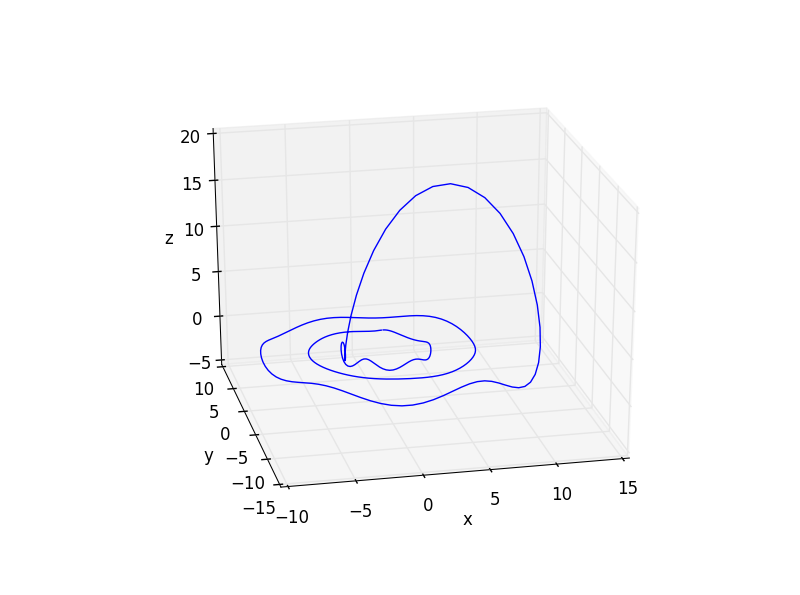
\includegraphics[width=\textwidth,height=.32\textheight]{MNGadjointinit}
\end{minipage}
\\
\begin{minipage}[height=.32\textheight]{.45\textwidth}
\centering \small{\texttt{(b)}}
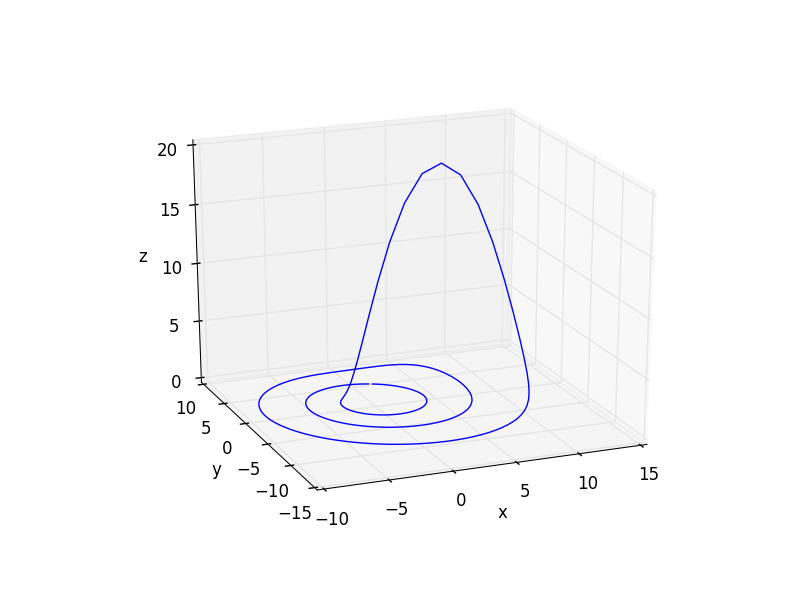
\includegraphics[width=\textwidth,height=.32\textheight]{MNGadjointfinal}
\end{minipage}
\begin{minipage}[height=.32\textheight]{.45\textwidth}
\centering \small{\texttt{(c)}}
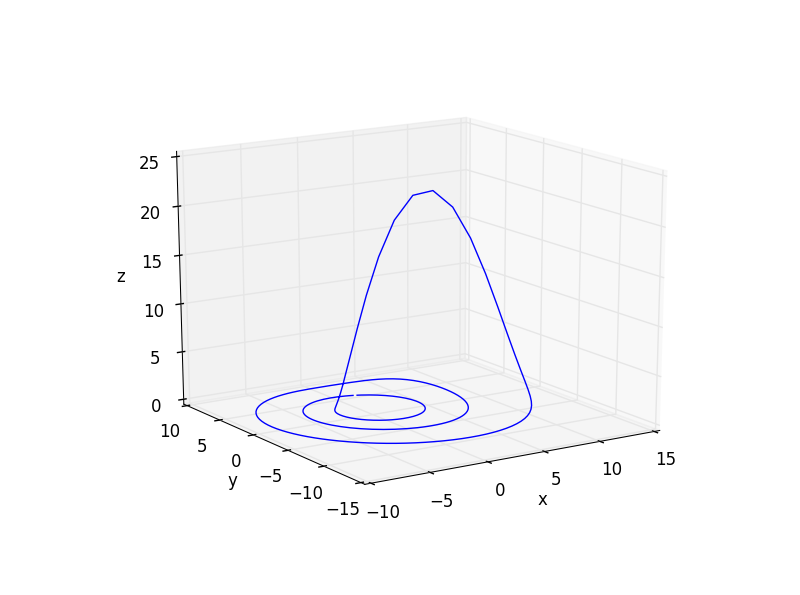
\includegraphics[width=\textwidth,height=.32\textheight]{MNGhybridfinal}
\end{minipage}
\caption{ \label{fig:MNGadjoint_hybrid}
(a) Initial condition for hybrid adjoint-{\descent} initial residual
of the spatiotemporal mapping $F^{2}_0 = 4.14084684359$.
(b) Output of the spatiotemporal adjoint method $F^{2}_{adj} = 0.0992808956991$,
(c) resulting spatiotemporal fixed point after applying Newton's method , $F^{2} \approx 10^{-15}$.
}
\end{figure}

\MNGpost{2017-10-04}{:
Finished up testing of Mohammad's adjoint method with lackluster sub-par results. Spent way too
long optimizing the method and trying to improve its speed. While the adjoint
method when applied to the spatiotemporal fixed point problem of the R\"ossler equations
does decrease the residual of the cost functional with the semi-norm of the mapping defined
by taking the discrete Fourier transform of the R\"ossler equation in time, the decrease
in the residual in minimal. This
is my claim after double and triple checking everything and comparing to straight-up Newton.

I think there is a use for it as a very crude preconditioner for Newton, or better yet Newton-Krylov hookstep.

When producing an initial condition based on close recurrences and using a Poincar\'e section, all but one coordinate
are likely to not be periodic; By taking a Fourier transform in time and setting the high frequency (some cut off in
mode number) the initial condition is smoothed out, but at the price of making the parameterized (now-smooth) loop
non-representative of the equations. By applying this adjoint method in conjunction with a crude tolerance, it can
be used to deform the initial condition into something more likely to converge with Newton.

Added quite a bit of functionality to the R\"ossler code but I'm just going to develop my own Newton-Krylov hookstep
code for R\"ossler now, unless there is some drastic change in my opinion about the adjoint method.
}

\PCpost{2017-10-08}{
I do not understand ``Krylov" in ``Newton-Krylov hookstep''
as applied to R\"ossler: If you are in 3~dimensions, what can Krylov do? Is the idea
that you are using numerical derivatives instead of using the exact

\MNGedit{The idea was to get the algorithms worked out for R\"ossler as even though there are only 3-dimensions, the spatiotemporal
system of equations one must solve to find Newton updates will have dimensionality $3M$ where $M$ is the number of time discretized
points, therefore for a long periodic orbit even in a small dimension system the dimensionality of the spatiotemporal system can
be as large as in \KSe\ if searching for very long orbits in R\"ossler, i.e. upwards of twenty Poincar\'e section returns. }
    }

\MNGpost{2017-10-06}{:
Some thoughts about numerical difficulties I have been facing. Predrag indicated that perhaps I should
look towards collocation methods as a numerical remedy for my situation. I don't mean to be picky but
I have been confused about this statement as Fourier (spectral) methods are collocation methods. The goal
is to find coefficients s.t. the solution can be written as an expansion in some basis, (i.e. a Galerkin
method is a collocation method with imaginary exponentials as the basis, Chebyshev Collocation is the
same but with Chebyshev polynomials as the basis.)

I think I have realized the difficulty with application of collocation methods with finding spatiotemporal
fixed points. The main problem in using spectral methods for this problem is that not only are we trying
to find the coefficients that minimize some residual such that the discretized solution exactly satisfies
the underlying equations, but when changing the domain size $L$ and period $T$ the basis functions (Imaginary
exponentials etc.) are ALSO changing. One might be able to get around this by creating a numerical
procedure that fixes the domain sizes, finds the best coefficients for that domain size, then allow the
domain size to change but this really isn't in the spirit of finding a spatiotemporal solution, we
would not like to constrain anything to change.

Therefore, I believe what perhaps Predrag is referring to is a method of relaxation, where all derivatives
are rewritten as finite differences between grid points.

\MNGedit{I am going to see if adjoint method works better in R\"ossler with using finite differences to approximate
the time derivatives now}
}

\MNGpost{2017-10-06}{
Reading my last post and realizing that I was conflating two different things; the way the what I was talking about
i.e. trying to match coefficients of a collocation method whilst changing the basis functions as well is essentially
is represented numerically by changing the values of a solution while also changing the domain size. I realized that
this is independent of the type of methods being used because numerically the affect of changing the domain size is
necessarily present in both types of methods. In other words I didn't think through it enough earlier.

Finite difference code adjoint code stalls just like Fourier code. I let an idea get to my head too quickly.

Ravi was kind enough to share a draft of his thesis which includes ways to speed up and improve adjoint descent, which
I am currently reading through.
}

\begin{figure}
\begin{minipage}[height=.32\textheight]{.45\textwidth}
\centering
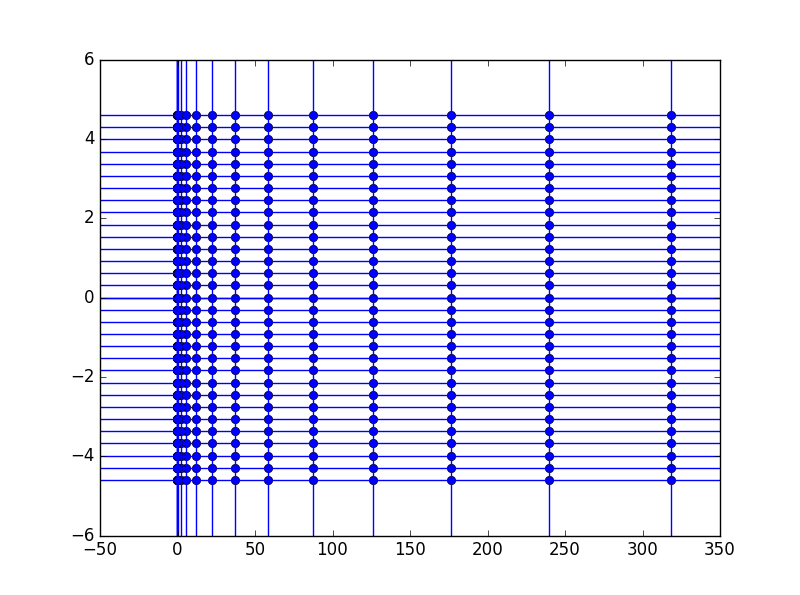
\includegraphics[width=\textwidth,height=.32\textheight]{MNGsttrivmult}
\end{minipage}
\caption{ \label{fig:MNGsttrivmult}
Spectrum of spatiotemporal multipliers associated with the linearization about the trivial solution
to the spatiotemporal mapping $F$. Plot is in the complex plane.
Vertical lines indicate the position of the values
$-q_k^2 +q_k^4$, horizontal lines indicate the position of $\pm w_\ell$, dots indicate
multipliers corresponding to this linearization.
}
\end{figure}


\MNGpost{2017-10-10}{:
The equations that I will describe are the spatiotemporal mapping described by discretizing the \KSe\ in
space and time, and then taking a spacetime Fourier transform that transforms the equations into a set
of nonlinear algebraic equations dependent on the spatiotemporal Fourier coefficients.

The next part of my formulation is to represent the indexed equations as matrix-vector products where
the vector is a $M*N$ dimensional vector (before taking care of continuous and discrete symmetries).
of spatiotemporal Fourier coefficients ordered in a a specific manner to be further elaborated on.

The matrices will be matrix representations of differential operators (time, space derivatives applied
to the spatiotemporal field of coefficients) or spatiotemporal discrete Fourier transforms.

If I may be so bold as to begin with the equations written in terms of the Galerkin truncation in space and
time of spatiotemporal Fourier coefficients;

I will denote the components of the mapping $F$ which is dependent on all of the spatiotemporal Fourier coefficients $\Fu_{k,l}$
as such:

\beq \label{e-MNGspattemp}
F(\Fu)_{k,\ell} = (i\omega_\ell -q_k^2 +q_k^4 )\Fu_{k,l} + iq_k/2 \sum_{\prime{k},\prime{\ell}} \Fu_{k-\prime{k},\ell-\prime{\ell}} \Fu_{k,\ell}
\eeq

Personally, I find it much easier in avoiding to mistakes to represent this mapping as matrix representations acting upon a spatiotemporal vector,
AND I have elected to represent the spatiotemporal Fourier coefficients by their real valued representations. The reason behind the real-valued
representations is that there are some underlying conjugacy conditions due to symmetries in the spectrum
such that the number of independent variables is far fewer than the total number of complex spatiotemporal Fourier coefficients, and I find
it easier to deal with these conditions in a real-valued representation. If one doesn't handle these conjugacy conditions then the linear
system of equations we desire to solve later will be singular and yield nonsense. In the words of Viswanath, "Determining the exact dimension
of the vector $x$ can be a little tricky because one needs to eliminate
Fourier coefficients that are conjugates of certain others and so on"\rf{Visw08}, I elect for simplicity which will hopefully be agreed upon after reading this.

Due to the ordering of the Fourier coefficients previously \emph{not} elucidated upon, the structure of the spatiotemporal vector will cycle through
all values of spatial index $k$ before changing the temporal index $\ell$. In a visual example this corresponds to
\beq \label{e-MNGstvec}
\transp{[\Fu_{k,l}]} = \transp{[\Fu_{k,0}, \Fu_{k,1}, \ldots, \Fu_{k,M/2}]}
\eeq
This notation can be somewhat confusing,especially more so when discrete symmetries
are taken into account, but hopefully I can clarify in this manner: When I take a spatial Fourier transform
with real-valued notation, then only half of the spectrum $k > 0$ is independent information. This is because the configuration
space field is real valued, the spatial Fourier coefficients
take follow the conjugacy rule $u_k(t) = u_{-k}^*(t)$.

In order to have a real valued representation these must be split between real and
imaginary components, i.e. $u_k(t) = a_k(t) + i b_k(t)$.

Now, $a_k(t)$ and $b_k(t)$ again constitute real valued series in time, so one follows the same procedure but in time (different ordering).

By doing so we can formulate differential operators to act on vectors with such an ordering,
in an absence of knowledge about naming conventions,

I will denote $W$ as the differential operator that, using spectral
differentiation, produces the time derivative of our spatiotemporal field; equivalent to multiplication of
the respective spatiotemporal Fourier coefficients
by $i \omega_\ell$.

$Q_1$ will denote
the differential operator that produces the second and fourth spatial derivatives, equivalent
to multiplication by $-q_k^2 +q_k^4$

$Q_2$ will denote
the differential operator that produces the first spatial derivative divided by two, equivalent
to multiplication by $i q_k / 2$.

$\mathcal{F}$ and $\mathcal{F}^{-1}$ will denote the matrix representations
of forward, and backward spatiotemporal Fourier transforms.

As to the explicit structures of these matrix representations, look further down.
With these definitions the nonlinear algebraic equation takes the following form.

\beq
F(\Fu) = ( W + Q_1) \Fu + Q_2 \mathcal{F} ((\mathcal{F}^{-1} \Fu)*(\mathcal{F}^{-1} \Fu)) \mbox{where} \, * \equiv \mbox{entrywise multiplication}
\eeq

For starters let us survey what linearizing about the trivial equilibrium $\Fu{k,\ell}=0$ yields.

\beq \label{e-MNGstlintriv}
\frac{\partial F(\Fu)}{\partial \Fu}|_{\Fu = 0} = W + Q_1 \equiv L
\eeq

The structure of $L = W + Q_1$ is copies of $-q_k^2 +q_k^4$ along the diagonal, and $-w_k$ on a
superdiagonal and $w_k$ on a subdiagonal.

The structure of $L$ is such that the multipliers take
the form $\Lambda_{k,l} = (-q_k^2 +q_k^4) \pm i w_\ell$, in addition to two marginal modes which should
are due to temporal and spatial translations. These two modes are dealt with by imposing two constraints.

In this regard. If we apply a perturbation to the trivial equilibrium, $\delta \Fu = \delta \Fu_{k=4,\ell=0}$
whose $L^2$ norm is reasonably small, then the spatiotemporal mapping yields $F(\delta \Fu) = (-q_4^2 +q_4^4)\delta \Fu_{k=4,\ell=0}$

This is relatively interesting as the spectrum of \reffig{fig:MNGsttrivmult}, if I am interpreting it correctly, seems to indicate
that somehow time is related to rotation while space is related to stretching.

A similar spectrum can be obtained for spatiotemporal fixed points
corresponding to {\ppo}s, except with some modulation in space due to the
nonlinear contribution. for {\rpo}s most of the structure is seemingly
lost. I don't have any results from antisymmetric orbits $\in \bbU^+$ but
I will try to provide an example of each tomorrow.
}

\MNGpost{2017-10-11}{
Proofreading Ravi's Thesis. Learning about his accelerated adjoint methods, Tried a bunch of silly things that I thought
would help the method converge but upon thinking about them I found myself wanting.

Plumbers meeting with more discussion about Burak and Akshunna's homoclinic orbits, accidentally muting people, Sadly I can't
remember the rest right now.

Talked with P.C. about the notion of spatiotemporal stability, Fuzzy Windows, Cat Maps, Invariants that everyone must be
able to reproduce.
}

\MNGpost{2017-10-11}{
\begin{description}
\item[Dynamical sampling talk]
Talk was hard to understand for someone without Mathematical training. I didn't really
understand what was going on for the most part because of the precise language he used.

What I got out of it is that in the context of viewing a Krylov subspace (he never
referred to it as such but that's what it was) as a "system"
in some sense you can show that certain properties of the operator are required in
order to show the Krylov subspace has properties such as being "complete" or being
a "frame" or its "Bessel-ness".

The most interesting part
was him using spectral decomposition of the operator to show that the Krylov
subspace is a "system" only if the eigenvalues are bounded away from zero and
near one. This is the general condition for when arnoldi iteration (more specifically
GMRES) will be a useful numerical method. Kind of interesting to see such different
language applied to something I have seen so often. The problem is I don't understand
what "system" means, I think it might be a linearly dependent basis?

\item[Cynthia Reichhardt]
\textit{Jamming and Clogging of Passive and Active Particles in Disordered Media}
Looking at the effect of density on clogging and jamming. Clogging is dependent on
some sort of geometry, Jamming isn't. Jamming is a phase transition described by
a diverging length scale, i.e. in a solid in order to move one particle you
would have to move them all.

Mentioning of some professor named Barringer whose experiments set the precedent
for the scaling ratios of binary mixtures of disks.

Assumption that motion of disks is overdamped is related to an assumption of friction,
but otherwise it is neglected.

Push a disk through 2-d nonhomogenous array of disks, look at how large its neighborhood
of interactions are. As density increase the neighborhood becomes global.

Now look at density of immobile disks. (previous example was one fixed disk limit).
Number of immobile disks decreases the jamming density. Corresponds to diverging length scale,
once length scales are equal they should cause jamming, but it turns out there is a critical
density of immobile disks that will cause jamming regardless of free moving disk density.

Takes a very long time to organize into a clogged state. I.e. an attractive fixed point with
very long transient times.

Clogged state described by anisotropy of the arrangement of free-moving disks and the transient
time it takes. Also there is a void that is typically normal to the direction of the motion.

Clogging states have a memory because the anisotropic voids created by one direction of
forcing will become pathways for movement if the direction of the forcing is changed due
to the lack of disks in that region.

To conclude, Jamming is a critical phase transition while clogging is a non-equilibrium
phase transtion.

Now moving on to active matter. Active in the regard that propulsion is an internal
mechanism. Specifically looked at run and rumble dynamics of bacteria such as ecoli.

Clustering of steric active particles, are velocities identical?

\end{description}
}

\MNGpost{2017-10-13}{:

While it's not lost on me that I spend too much time learning numerical methods and
not enough Physics, this is what I have to do to get anywhere it seems.

\begin{description}
\item[ravi thesis]
Finished proofreading Ravi's thesis and learning the material within.

\item[Adjoint improvements]
Implemented changes to adjoint code that include the following combinations

\begin{itemize}
\item Ravi's iterative method
\item Ravi's "rotation" method. (It's preconditioning)
\item Momentum term from Nesterov
\item (still crude) adaptive time stepping for RK4
\end{itemize}

I'm still tinkering with different combinations and definitions for all of these that
maximize speed. The improvements are relatively different from Ravi's at this point, in
about the same computation time as before I only manage to get an order of magnitude
improvement over my previous methods when applied to the R\"ossler system. In the scope
of the larger problem which is spatiotemporal \KSe\ this might do fine because most
of the work should be done by Newton, we only need to get within a region where Newton
will converge.

The general idea behind Ravi's "rotation" method is that there are some Fourier modes
that are slowly changing in fictious time, so we want to maximize the change of
these modes in any numerical algorithm we implement. His explanation of the method
he decides to use and the justification falls in line with most justifications
I have read for using preconditioning in any iterative or descent method, which is,
namely, that it varies from problem to problem and unless the structure of the matrix
from the linear system has a specific structure, then the choice of preconditioner
falls to intuition and other dark arts.

Yurii Nesterov is a Russian Mathematician who has made great strides in convex optimization
and some of his papers have thousands of citations due to their impact on numerical algorithms
corresponding to improvements in speed\rf{Nesterov83}. The classical text on the subject however seems to
be Boyd and Vandenberghe 's \textit{Convex Optimization}\rf{BoyVan04}. If anyone is interested
there are also video lectures on Convex Optimization done by Stanford with Stephen Boyd as the
lecturer, He's a very enthusiastic and insightful lecturer so it's good to put on in the background
while doing menial tasks. \HREF{https://www.youtube.com/playlist?list=PL3940DD956CDF0622}{video lectures}.
Also the book is available for free on his personal website \HREF{https://web.stanford.edu/~boyd/cvxbook/}{book}.


\item[spatiotemp]
Spent some time trying to think of a way to exploit symmetries in the spectrum
of spatiotemporal (Floquet in this case?) multipliers. I haven't come up
with anything as of yet.

\item[Julia]
Began reading the documentation of Julia as a means to increase the speed
of Python code.


\end{description}
}

\MNGpost{2017-10-17}{:
Implemented the accelerated adjoint method for \KS. The initial performance
on test cases was very good but for general initial conditions generated by close
recurrence the performance still needs to be improved.

The general description of the adjoint method is that we are stepping
in fictitious time determined by $-\transp{J(\Fu)} F(\Fu)$ as this ensures that
the cost functional will monotonically decrease to $0$. The description of the improvements
can be summed up by the following.

The linear component of the spatiotemporal mapping, and thus the contribution
to the \jacobianM\ is dominated by the contribution by the Laplacian and
Laplacian squared terms of the \KSe. The way it presents itself in the
contribution to the \jacobianM\ of the mapping is to have a dominant
diagonal. This is one of the instances where use of a diagonal (Jacobi)
preconditioner is motivated.

This is implemented by introducing the preconditioning matrix $M$ such that the new adjoint direction
is given by  $\partial_\tau \Fu = -M\transp{J}(\Fu) F(\Fu)$

This has its benefits for this system but there may be an even smarter choice hiding out somewhere.

The other advancement is described in (its a secret Russian paper that only few may read apparently)
\rf{Nesterov83} that proves that by including a 'momentum' term in the iterative process, then
the descent process can be sped up by including a contribution from the previous fictitious time
direction. The algorithm that this manifests in is given by

\bea \label{eqn:Nesterov_factor}
\mu_0 &=& 1 \continue
\mu_k &=& \frac{1 + \sqrt{1+4*\mu_k^2}}{2} \continue
\delta \Fu_{k+1} &=& \delta \Fu_k + \frac{\mu_k-1}{\mu_k +1} \delta \Fu_{k-1}
\eea

If the residual increases then the momentum is restarted at $\mu = 1$ and the iterative
procedure begins again.

Just to reiterate, I have implemented these methods for spatiotemporal \KSe\ and it can
take a (relatively) arbitrary initial condition and descend it to reduced the residual.

Now specifically, I haven't found an initial condition that the full hybrid process
in conjunction with Newton works yet. So the next steps are to implement Newton-Krylov
hookstep methods (finally getting to it after everything else) and clean up the initial
condition generation code (which I started today).

If both of these changes does nothing then the last resort will be to pass close recurrence
initial conditions to a Newton-descent in time in order to give one of the tangent spaces the
correct shape before starting the spatiotemporal hybrid descent.

The other option is to let the adjoint descent run for arbitrarily long times, but I'm not
convinced this is helpful. We shall see.

}

\MNGpost{2017-10-21}{:
\item[spatiotemp]
Almost finished with the Newton-Krylov hookstep method, reading Dennis and Schnable
\rf{Dennis96} for the best way to calculate the trust region among other things.

The first implementation worked with Givens rotations such that the Hessenberg
matrix produced via arnoldi iteration was transformed into an upper triangular
matrix, thereby making the nonlinear optimization part of GMRES easy to solve,
or so the resources say.

I have opted to just use a least squares solver on
this part, and a blackbox nonlinear solver to calculate the optimal hookstep
direction, as they tend to be easier to code.

\item[Mohammad Conversation]
Mohammad posed the idea at the last plumbers meeting that I should just derive
the spatiotemporal adjoint equations and then use these to compute the adjoint
direction instead of explicitly forming the \jacobianM\ and computing
$G(\Fu) = -1 \,\transp{[\nabla F(\Fu)]} F(\Fu)$. We shared ideas back and forth,
all of my ideas ended up in required that we had already discretized the equations,
which is what we were trying to avoid; He mentioned that when he made the statement
he thought it shouldn't be too hard but in our conversation it was non-trivial
and more complicated then he had anticipated. To this end, no real progress was
made on my end after thinking about this for a while.

\item[adjoint misc]
Tried playing around with some other numerical procedures that I thought would help
the adjoint, but I was either not careful enough when implementing them or there
is something else at play. For instance, I tried implementing dealiasing the nonlinear
computation to make them more accurate but this really wasn't well received by
my spatiotemporal adjoint descent code.


}

\MNGpost{2017-10-24}{
\item[numerics]
Almost done with the hybrid methods, will be posting statistics hopefully before
tomorrow's meeting.

The spatiotemporal fixed point code now has the ability to run the following numerical
methods in searches.

\begin{itemize}
\item Hybrid Preconditioned Adjoint-Momentum-Descent Newton-Krylov hookstep (Main method)
\item Newton-Krylov hookstep
\item Damped Newton (For really good initial conditions)
\item Undamped Newton (For really good initial conditions)
\item Preconditioned Adjoint Descent
\item Raw Adjoint Descent
\item Momentum accelerated Adjoint Descent.
\end{itemize}

Standalone Adjoint Descent code, (Preconditioned, accelerated) should be used if the numerical residual
isn't too important and one just wants a fuzzy window/smoothing out an close recurrence guess.

Standalone Newton Method Type procedures should only be used if the initial condition is
exceedingly close to a spatiotemporal fixed point (at least in the case of damped, raw Newton, still
need to test the hookstep).

A little work needs to be done on the following before I can proclaim \emph{Ta da!}.

\begin{itemize}
\item Automated Initial condition generator is still a little rough around the edges.
\item The focus on numerical methods has lead me astray from the time parameterization for {\rpo} fixed
points
\item The trust-region calculation and general comments in the hookstep code need to be improved.
\item Numerical statistics need to be introduced to determine the efficacy of the various methods
versus each other.
\item Another constraint needs to be implemented for \ppo\ fixed points, the current code utilizes
constraints on the Newton steps such that they are orthogonal to time,space equivariance, however
in the \ppo\ case the direction of spatial equivariance is an impossibility due to the
peculiar form of the Fourier transforms used that exploit the discrete symmetry. ( I just realized
this today, it turns out that by keeping the terms I did I believe I might have 'accidentally'
quotiented the $\SOn{2}$ symmetry, when I thought I was getting rid of the reflection symmetry.
Still looking into maybe this is close to quotienting $\On{2}$. Currently as a work around I am using
something ill-advised (constraining the steps to be orthogonal to the $2nd$ and $4th$ spatial derivatives
with no motivation to do so except it improved performance.
\item Preconditioning for the arnoldi iteration portion of the hookstep code should probably be
implemented, as it helps a lot for the adjoint descent.
\end{itemize}

In regards to the comments about quotienting $\On{2}$ for {\ppo}s. I've been thinking a lot about it today and
trying to utilize some of the teachings of my adviser (Gasp) to try to think about symmetries spatiotemporally.
I'm trying to reconcile the fact that the reflection symmetry present in \ppo\ fixed points can be inverted by
translating by the period of the fundamental domain. (i.e. $R u(x,t) = u(x,t + T_p)$


}

\MNGpost{2017-10-26}{
\begin{description}
\item[automated initial condition generation]
Still debugging the {\rpo} part of this code, might include the ability to pass the initial
condition to a {\descent} in time just to smooth out and or correct the tangent space
before sending it to spatiotemporal problem (My last resort if I can't get it to work for
spatiotemporal initial conditions produced by close recurrence).

\item[janitorial duties]
The spatiotemporal fixed point code has grown to an extent that it is becoming far too unwieldy and
some of the functions defined by me were done without a thought as to what to call them.

Most of my time today was spent splitting the file with all of the function declarations into
a number of pieces, and keeping the numerical methods separate. This isn't exactly progress
but I'm hoping it will speed things up in the future. As it was previously written, for each
numerical method I needed a separate function depending on the symmetry (isotropy subgroup,
stabiliser, etc) of the initial condition. Now that most of the numerical methods are working
I am trying to rewriting them to be independent of the symmetry of the solution other than
a keyword argument ((switch,flag) for those who use command prompt to run scripts.) The reason
it was written this way is because I had to formulate it in terms of test-cases and so usually
I choose a certain subgroup to work in at first.

\item[hookstep]
Reading Dennis and Schnable\rf{Dennis96} to improve the trust-region calculations for hookstep,
it all seems sort of heuristic to me but I'm sure there are rigorous proofs elsewhere that I wouldn't
understand. Confusing as well. The general idea is that because of the specific form of an equation
to calculate the optimal hookstep, Newton's method in the free parameter is suboptimal, so they
introduce lower and upper bounds on the trust region and a modified linesearch and also a quadratic
model to test the accuracy of the hookstep. Seems to be needed as John did it as well.

\item[failed attempt]
I thought perhaps that perhaps applying the adjoint descent on a fixed spatiotemporal area would help
poor initial conditions converge, but the adjoint descent really doesn't seem to agree with a fixed
'window'. The idea is that before approaching the full spatiotemporal problem, we should really correct
the tangent space first.

\item[other spatiotemp implementations]
Still improving functionality of the code and some small numerical procedures.
During the rewrite I wrote pieces of code to apply least squares to the Newton method procedures
to avoid constraints that seem to vary in there efficacy.

Here's a short list
of things I am trying to get done:

\begin{itemize}
\item Dealiasing using 3/2 rule, via prolongation and contraction matrices (spatiotemporal zero-padding)
\item Constraint-type keyword arguments
\item Preconditioned GMRES
\item Statistics on the numerical procedure (i.e. Residual of Cost Functional versus computation time, iterations, function calls, etc.
\item Statistics and or plots of spectra and eigenvectors of spatiotemporal \jacobianM
\item Trying to think of spatiotemporal invariants to perhaps use as axes in plots
\end{itemize}


\end{description}
}

\MNGpost{2017-10-30}{
\begin{description}
\item[spatiotemp code]
Finished the reorganization, added some functionality by means of being able to plot
residual versus iteration number for different methods. Included preconditioning matrices
for {\rpo} and antisymmetric orbits $\in\bbU^+$.

\item[spatiotemp initial conditions]
Still debugging this. Narrowed down the problems to taking too large of steps in the
integrator and something ill defined in the Poincar\'e section piece of code.

\item[Schatz and Grigoriev Group]
By request of Ravi, I presented some results of the adjoint method and discussed
how it was implemented for my spatiotemporal problem. Most of the questions came
from Roman G., Mike Schatz, Kimberly S. Roman was concerned about the marginal
directions and whether or not solutions exist.

\end{description}
}

\begin{figure}
\begin{minipage}[height=.32\textheight]{.45\textwidth}
\centering \small{\texttt{(a)}}
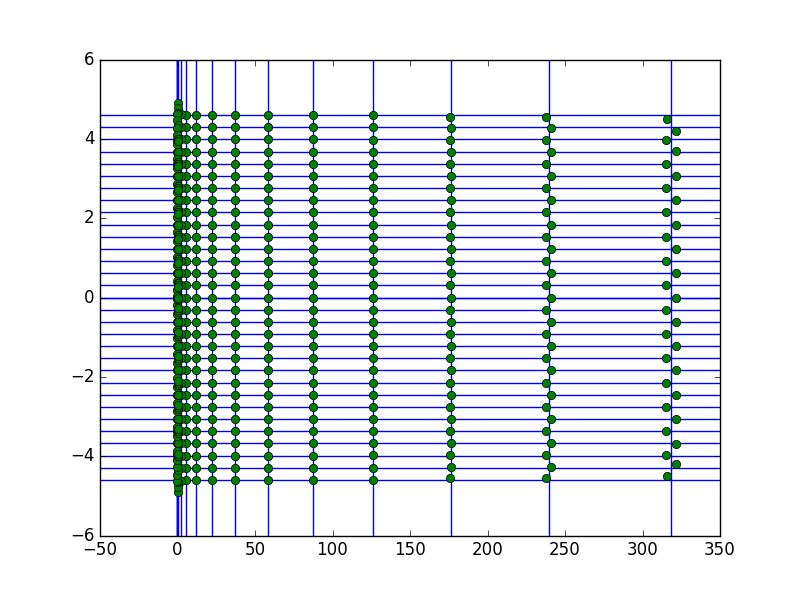
\includegraphics[width=\textwidth,height=.32\textheight]{MNGppo1_spectrum}
\end{minipage}
\\
\begin{minipage}[height=.32\textheight]{.45\textwidth}
\centering \small{\texttt{(b)}}
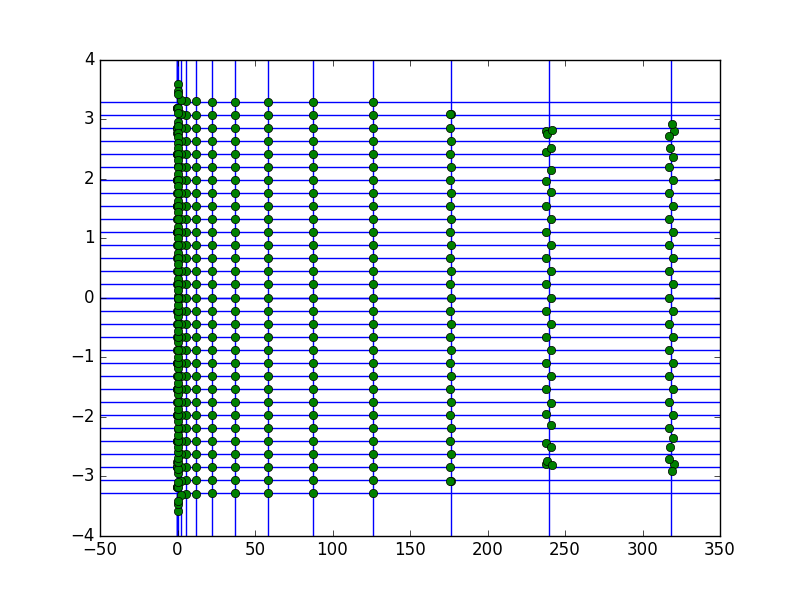
\includegraphics[width=\textwidth,height=.32\textheight]{MNGppo2_spectrum}
\end{minipage}
\begin{minipage}[height=.32\textheight]{.45\textwidth}
\centering \small{\texttt{(c)}}
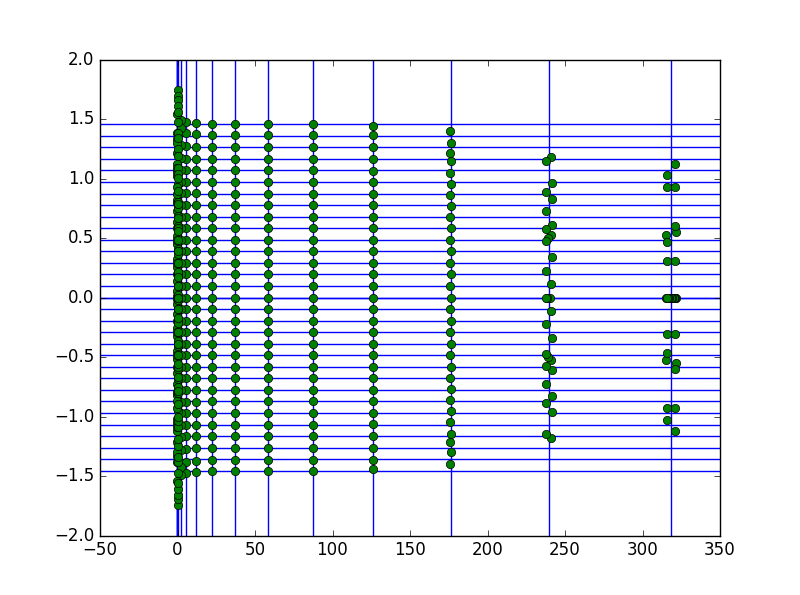
\includegraphics[width=\textwidth,height=.32\textheight]{MNGppo3_spectrum}
\end{minipage}
\caption{ \label{fig:MNGppospacetimespec}
(a) Spatiotemporal multiplier spectrum for \PPO{10.2},
(b) Spatiotemporal multiplier spectrum for \PPO{14.3},
(c) Spatiotemporal multiplier spectrum for \PPO{32.3}.
Intersections between horizontal and vertical lines indicate where the
multipliers would be for the $u(\conf,\zeit)=0$.
In other words, changes from this grid indicate
differences between the linearized spatiotemporal spectrum and the full
spatiotemporal spectrum. All three solutions converged to within machine
precision when defined on a 32-by-32 spacetime grid; Fourier calculations
done with $15 \times 31$ spatiotemporal Fourier coefficients.
}
\end{figure}


\MNGpost{2017-10-31}{
\begin{description}
\item[spatiotemp]
Fixed some bugs related to keyword arguments. All numerical methods are now independent
of the particular type (isotropy subgroup) of solutions other than keyword argument
"symmetry". Included default values for tolerances, dimension of Krylov subspaces, adjoint
fictitious time, and etc. so that other users don't have to think worry about specifics if
they just want black box numerical algorithms to work with.

Still working on improving the hookstep algorithm, as well as initial condition generation code,
the initial conditions specifically need to be pretty precise or else the spatiotemporal convergence
will not work. The hookstep improvements are just confusing as all hell to me.

The general procedure is to use a modified Newton search for the optimal hookstep; Using John's
code as a guide I've realized there are quite a few more additions than I orginally thought
that need to be made before I can say it's "done".

\item[initial conditions]
Still trying to figure out the bug regarding Poincar\'e sections, will hopefully find by the
end of the day. For \ppo\ I am constructing Poincar\'e sections based on the reflected partner
of the initial point returned by close recurrence. I.e. for an initial condition $u(\conf,0)$
I am attempting to produce initial conditions that shadow {\ppo}s by constructing a hyperplane
whose template point is the reflection operation (performed in Fourier space) $R u(\conf,0)$.
and then defining tangent and normal vectors to the plane based on the first Fourier mode.

\item[misc]
Realized that my damped Newton is actually equivalent to backtracking line-search type Newton
due to the fact that I keep reducing the step size until I find a correction that reduces
the residual, instead of just using a reduced step-size Newton.
\end{description}
}

\MNGpost{2017-10-31}{
Trying to see if there are any way to use the initial spatiotemporal spectra that would
determine if a solution will converge or not. For instance, for the tenth shortest \ppo\
I needed to use a 32-by-64 space by time discretization to get it to converge. I.e.
I had to increase it by a factor of two.

It should be noted that this factor of two is what I chose not because it was the smallest
increase but rather its the convention I'm used to due to the fact it improves the performance
of FFTs. Now, because I was more focused on accuracy rather than performance, I have implemented
these so-called direct-matrix methods. I.e. I am explicitly forming everything in terms of
matrices and vectors, so I believe that as long as I retain even numbers my code will run,
meaning that I do not have to sacrifice much performance to improve the discretization,
because I only have to perform the FFTs (forwards and backwards, space and time) once.

I'm going to be testing this in the future, something along the lines of: If convergence fails,
increase the time discretization by two, four, etc. For the spatial discretization there doesn't
seem to be such an issue due the fourth spatial derivative, but when I get to large domains
I will likely have to make some adjustments there as well.

Still improving hooksteps, can't really get this optimization using Lagrange constraints via \refref{Dennis96}
to work.

}

\MNGpost{2017-11-02}{:
\phantomsection\label{2017-11-02MNG} % refer to it by
% on page~\pageref{2017-11-02MNG}
Reading about trace formulas and zeta functions makes me think I should rewrite my equations
such that everything is a fixed point with period one. Right now I guess you could say that
everything is represented by fixed points of period two, because $F(\Fu)=0$, not $F(\Fu)=\Fu$.

In this case then the general formulae I have been using would only need to be tweaked in a relatively
small manner. In order to formulate a function that follows $G(\Fu) = \Fu$, we need to do some rearrangement
in the spatiotemporal equations I have been utilizing. (Also, I'm going to switch up the conventions I have been
using for almost a year now to something more recognizable by the reader).

In what follows $D_i$ are differential operators with respect to the index, and $F$ are spatiotemporal Fourier
transform operators.
\beq
(D_{\zeit} - D_{\conf \conf} + D_{\conf \conf \conf \conf})\Fu + D_{\conf}F((F^{-1} \Fu)^2) = 0
\eeq
Noting that the operator that equates to the difference
of the second and fourth spatial differentiation operators is diagonal, and not singular by construction, we can
easily take the inverse of the operator (because it's diagonal), and we arrive at the equation
\beq \label{eqn:MNGspacetime_reform}
G(\Fu) = (D_{\conf \conf} - D_{\conf \conf \conf \conf})^{-1} (D_{\zeit} \Fu + D_{\conf}F((F^{-1} \Fu)^2)) = \Fu
\eeq
This might be the ``proper" way of doing things, even numerically, because this essentially scales out the large
spatial components due to the fourth order term.

I'm still learning (slowly) the methodology and intuition behind trace formulas and zeta functions but this might
be the proper way of viewing things because then all doubly periodic orbits are in fact spatiotemporal fixed
points as opposed to period two orbits. (in other words instead of a string of symbols $\bar{N} \bar{0} \bar{0} \dots$
in the fictitious dynamics introduced by applying the mapping function, I am instead identifying the orbit by just $\bar{N}$,
where $N$ is a label given to spatiotemporal fixed points.)
}

\MNGpost{2017-11-07}{
In reference to the post of {\bf 2017-03-14},
%\phantomsection\label{2017-03-14MNG} % refer to it by
on page~\pageref{2017-03-14MNG}
in \refchap{chap:dailyBlog}~{\em
Space-time, blogged} I would argue that what I have done is quite similar to
L{\'o}pez \etal\rf{lop05rel}.

By using the spacetime Fourier-Fourier basis representation of the spatiotemporal field with
Galerkin truncations in space and time
\beq   \label{eqn:mng_am_ansatz_ks}
    \am{m}(t)  =  \sum_{n \in \integers} \akj \e^{\ii \omegaj t} \, ,
\eeq
The nonlinear algebraic equations in this basis are \refeq{e-FksSpattemp}.
I will restate the equations here
for completeness and comparison to L{\'o}pez \etal\rf{lop05rel}.
In the spacetime Fourier-Fourier basis, the \KSe\ takes
the form,
\beq
\left[ \ii \omegaj - ( \wavek^2 - \wavek^4 ) \right] \akj
+ \frac{ \ii \wavek }{2} \!\sum_{k'} \sum_{j'}\!\!
\akj a_{k-k',j-j'}
    = 0
\,.
\ee{FkSpattemp}
while in L{\'o}pez \etal\rf{lop05rel}, with the ansatz for {\rpo}
solutions \refeq{eqn:am_ansatz} the \cGL\ take the form
\bea
\ii \left( \frac{2 \pi n}{T} - \frac{\varphi}{T} - m \frac{S}{T} \right)\,\akj
    &=&
    R \akj  - m^2 (1+\ii \nu)\akj
    \label{eqn:spacetime_lop05rel}\\
    - (1+ \ii \mu)\sum_{m'}
      \sum_{n'} a_{k_1,j_1} a_{k_2,j_2} a_{k_3,j_3}^{*}
\,,
\nnu
\eea
where $m_1+m_2-m_3 = m'$ and $n_1+n_2-n_3 = n'$.

The differences between our methods arise when setting up the equation as a root
solving procedure. In L{\'o}pez \etal\rf{lop05rel} the numerics is handled by solving for the
roots of the function $F(\akj ,\varphi , S, T) = 0$ where $F$ is the function described
by \refeq{eqn:spacetime_lop05rel} if one moved all of the terms to one side of the equation.

In my current procedure, I solve
\refeq{e-FksSpattemp}, % PC: Matt had here {eqn:FksSpattemp}
or for comparison,
$F(\akj, T, L) = 0$, where $T,L$ are in the factors $\omegaj,\wavek$ respectively.

I do not explicitly include variables that control the spatial translations of the system and,
up until now, have elected to search for {\rpo} solutions pertaining to
\refeq{e-FksSpattemp} % PC: Matt had here {eqn:FksSpattemp}
by finding them in the first Fourier mode slice. Part of the reason of this was I didn't
understand the reasoning behind parameterizing the spatial translations by $\zeit$ by means
of the factor in the ansatz $\e^{-\ii \wavek \frac{S}{T}t}$. I thought the shift factor
had to be explicitly calculated by the coordinates, and not assumed through this type of time
dependence.

My comments of
{\bf 2017-11-02} on page~\pageref{2017-11-02MNG}
were mainly predicated by the fact that once we find these roots, I don't think
we can apply the same type of reasoning as Politi and Torcini\rf{PolTor92b} as
they aren't truly fixed points of a fictitious dynamical system, like so,
$F(\akj, T, L) = {\akj, T, L}$. But rather, like I have already
described, they are the roots of a system of nonlinear algebraic equations,
$F(\akj, T, L) = 0$.

If I am so inclined to change how I search for relative periodic orbits in the same manner as
L{\'o}pez \etal\rf{lop05rel} I believe all I would have to actually implement is this $\e^{-\ii \wavek \frac{S}{T}t}$
factor in my ansatz, such that the new equations for solutions with $\SOn{2}$ symmetry would be,
\beq
\left[ \ii \omegaj - m \frac{S}{T} - ( \wavek^2 - \wavek^4 ) \right] \akj
+ \frac{ \ii \wavek }{2} \!\sum_{n'} \sum_{m'}\!\!
\akj a_{k-k',j-j'}
    = 0
\,.
\label{eqn:FksSpattemp_rel}
\eeq
such that the spatiotemporal solutions would now be roots of the nonlinear system of equations,
$F(\akj, S, T, L) = 0$

}

%\PCpost{2018-01-20}{
%Moved Matt's Politi and Torcini\rf{PolTor92b} blogposts
%to \texttt{blogCats}, dailyCats.tex.
%% Predrag 18 April 2020 returned to siminos/spatiotemp/blog.tex
%    }

\MNGpost{2017-11-08}{
\begin{description}
\item[plumbers]
Second part of plumbers meeting was about discussing
why averaging over a line in the infinite spatiotemporal
case is fundamentally different than looking at a finite
rectangle or strip. The latter imposes both length and time
scales likely different than how nature would impose them
and hence any statistics gained would be necessarily different.

\item[conversation with Andy]
Discussed variational methods, Jianke Yang's code, and
applications to Graduate school at length with Andy.

\item[Jianke Yang]
Read through the code and ran it, the hybrid Newton and
conjugate gradient descent can reach a tolerance value of
$10^{-10}$ pretty easily, taking only seconds to run; but when
the tolerance is made more strict then after experimentation
with it, it doesn't converge even after running for hours; I might
be missing something numerically but I guess I'm trying to test his
algorithm against the same standards I'm holding my algorithms.


\end{description}
}

\MNGpost{2017-11-13}{
{\bf Jianke Yang spatiotemp}
I'll try to outline Jianke Yang's paper\rf{Yang15}

He begins with an exposition about the previous work specifically
Lan and Cvitanovi{\'c}\rf{lanVar1} and L{\'o}pez \etal\rf{lop05rel}, which are two of the main papers I work
around so there's likely something I can take from this paper.

Jianke Yang has the following to say about working with an infinite tower of ODEs versus PDEs.

\begin{quote}
In this article, we develop a new numerical method for computing
time-periodic solutions in dissipative wave equations. This work is motivated by several reason. First, our view is that the best way
to compute such solutions in PDEs is to do so in the PDE framework,
rather than converting PDEs to large systems of ODEs or algebraic
equations. The advantage of the PDE framework is that the structure
of the PDE is retained, and important quantities such as the
linearization operator of the PDE can be calculated analytically.
Second, almost all numerical methods for time-periodic solutions
in PDEs involve solving lare systems of linear equations. Since
conjugate-gradiate methods are widely recognized as probably
the fastest numerical method for solving linear algebraic
and operator equations, we are motivated to incorporate conjugate-
gradient methods into our algorithm.
\end{quote}

He says that he prefers to work in the "PDE framework" but he uses
spectral code to compute all derivatives (due to the accuracy of
spectral methods versus finite differences). I don't buy the
comment about working in the "PDE framework". He is making it sound
like he doesn't use the ODEs in Fourier space but this is exactly
what he is doing when he uses them to compute spatial and temporal
derivatives. In other words the basis for his claim for working
in the "PDE framework" is that he solves the resultant linear system
(via a combination of Newton and conjugate-gradient)
in physical space versus Fourier space.

If I had to rephrase these comments I would say that he finds it
advantageous to compute all terms pseudospectrally; the derivatives
are computed in spectral space but the linear system of equations that
arise are solved in physical space. His claim that "no truncation to
ODEs or algebraic equations is necessary" is \emph{nonsense}. That's exactly
what is necessary in order to compute the derivatives spectrally.

Another difference between his code and my own is to use "quasi Rayleigh
quotients" to determine free parameters. (e.g. the period of the solution).

For example, to determine the period of periodic solutions of the
\KSe\ he rescales time $\tau = \omega \zeit$ such that $0 \leq \tau \leq 2 \pi$, such that the PDE can be rewritten as,

\beq \nonumber \label{e-Yang15pde}
\omega u_{\tau} = F ( \conf, \partial_{\conf}, u) \mbox{where,} \, \tau = \omega \zeit
\eeq

and then rewrite $\omega$ in terms of the solution itself via the so
called quasi Rayleigh quotient,

\beq \nonumber \label{e-Yang15omega}
\omega = \frac{< u_{\tau}, F > }{< u_{\tau},u_{\tau}>}
\eeq

such that the original equation now takes the form,

\beq \label{e-Yang15}
\frac{< u_{\tau}, F > }{< u_{\tau},u_{\tau}>} u_{\tau} - F ( \conf, \partial_{\conf}, u) = 0
\eeq

Due to the inner products (defined as the spatiotemporal $L_2$ inner product) the equation to solve now takes an integro differential form,
but he says that this price is worth paying for.

He then derives analytic equations for the linearization of \refeq{e-Yang15}, which is going to be the linear system that is
going to be solved to yield the Newton corrections.

In order to apply his Newton conjugate gradient method, he needs
to transform the system such that it becomes self-adjoint, but I feel
that any exposition into this likely would not be helpful for discussion
as its all numerics at this point. He does however mention the practicality of preconditioning the linear system, which is something
that I have been debating.

{\bf Further derivations}

Due to the fact that J. Yang is writing the spatiotemporal equations
as a root finding procedure, a linear expansion will be required
to set up the system of equations that need to be solved in order to
step in the correction direction (If one thinks about it in the scope
of Newton's method, we need to be able to linearize about the root
such that we derive a linear system of equations whose solution is
the Newton correction).

Due to the presence of this time-rescaling factor $\omega$ and its
explicit definition in terms of the so called quasi Rayleigh quotient,
in order to linearize the equation \refeq{e-Yang15} about a root, we need to derive the expression for the linearization
of $\omega(u) = \frac{< u_{\tau}, F > }{< u_{\tau},u_{\tau}>}$.

In other words, we need an expression for $\omega(u + \delta u)$. To
get a useful form of this equation, we first use the fact that we know
the linearization for the function $F$.

\bea
\omega(u + \delta u) &\approx& \frac{< (u+ \delta u)_{\tau}, F(x,\partial_x, u + \delta u) > }
                                {< (u+ \delta u)_{\tau},(u+ \delta u)_{\tau}>} \continue
\omega(u + \delta u) &\approx& \frac{< (u+ \delta u)_{\tau}, F(x,\partial_x, u) + F_1 \delta u > }
                                {< (u+ \delta u)_{\tau},(u+ \delta u)_{\tau}>}\,,
\eea
where $F_1$ is what Yang calls the ``linearization operator" but others would recognize it as the
\jacobianM.

We can simplify this expression by substituting the equality given by \refeq{e-Yang15pde},

\beq
\omega(u + \delta u) \approx \frac{< (u+ \delta u)_{\tau}, \omega u_{\tau} + F_1 \delta u > }
                                {< (u+ \delta u)_{\tau},(u+ \delta u)_{\tau}>}
\eeq

And then just for add and subtract $\omega \delta u_{\tau}$ in order to separate into two terms,

\beq
\omega(u + \delta u) \approx \frac{< (u+ \delta u)_{\tau},
                                \omega (u+\delta u)_{\tau} + (F_1 - \omega \partial_{\tau}) \delta u > }
                                {< (u+ \delta u)_{\tau},(u+ \delta u)_{\tau}>}
\eeq

After keeping only first order terms in $\delta u$ we get,

\beq \label{e-Yang15linearomega}
\omega(u + \delta u) \approx \omega -  \frac{< u_{\tau},
                                    (\omega \partial_{\tau} - F_1) \delta u > }
                                {< u_{\tau},u+ \delta u)_{\tau}>}
\eeq

The whole point of this exercise was to describe the linearization of the equation whose roots
will result in doubly periodic solutions, namely \refeq{e-Yang15}.

To derive the expression for the \jacobianM\ of \refeq{e-Yang15} we will use the decomposition
elucidated in \refeq{e-Yang15linearomega}. This can be explained by the following equations,

\bea
L_0 (u) &=& \frac{< u_{\tau}, F > }{< u_{\tau},u_{\tau}>} u_{\tau} - F ( \conf, \partial_{\conf}, u)
        \continue
L_1 &\equiv& \frac{\partial L_0}{\partial u} = (\omega \partial_{\tau} - \frac{\partial F}{\partial u}) + \frac{\partial \omega}{\partial u} u_{\tau}
        \continue
L_1 &=& (\omega \partial_{\tau} - F_1) - \frac{< u_{\tau},(\omega \partial_{\tau} - F_1)> }{< u_{\tau},u_{\tau}>} u_{\tau}
        \continue
P &\equiv& (\omega \partial_{\tau} - F_1) \Rightarrow
        \continue
L_1 \delta u &=& P \delta u - \frac{< u_{\tau},P \delta u> }{< u_{\tau},u_{\tau}>} u_{\tau}
\eea

With this definition we can then solve by iterative methods the system of equations given
by,

\beq
L_1 \delta u = -L_0 \, ,
\eeq

such that when when $L_0 = 0$ we have found the solution.

This is the general derivation for one extra parameter (in this case $\omega$, which is a taking the place of period),
the general derivation for a two parameter case (which is necessary to allow period and domain size to vary) is the
next undertaking.

}

\MNGpost{2017-11-13}{
\begin{description}
\item[initial condition generation]
In order to reduce the number of garbage initial conditions,
we first pass through a close-recurrence problem that sifts
through en ergodic trajectory for a possible place that we
can set up a Poincar\'e constraint. This is done
by time-integration followed up by computing $||u(x,t_0) - \sigma u(x,t_0 + \tau)||$
where $\sigma$ is the relevant symmetry operation for the type of orbit we
are searching for.

The current Poincar\'e procedure can be defined by the following:

For an example point defined by its spatial Fourier coefficient
representation $u(x_n, 0) = \sum_{k} (a_k + \ii b_k ) e^{i q_k x_n}$,

For \ppo\ solutions,
I define a Poincar\'e section whose template point is the reflection
of the real component of the first Fourier mode. Namely,

$\Fu_{template}  = \transp{[0 -a_1 0  0 \dots -a_{1}]}$

Note: $a_{1} = a_{-1}$ by conjugacy symmetry of Fourier coefficients of
real valued function.

Then the Poincar\'e section constraint is defined by this template point,
as well as the transverse component of the velocity evaluated at the
spatial reflection of our starting point, or written as an equation,

\beq
U(\Fu) = <\Fu_{template} - \Fu | \hat{n} > \mbox{where,} \quad
\hat{n} = \frac{v(R \Fu) - <v(R \Fu)|\hat{t}> \hat{t}}{||v(R \Fu) - <v(R \Fu)|\hat{t}> \hat{t}||}
\eeq

In order to ensure that the transversality condition is always to find $U(\Fu) = 0$
between the two points $U(\Fu_{n-1}) < 0,U(\Fu_{n}) > 0 $, we include the orientation
of the velocity in the definition of $\hat{n}$.

\end{description}
}

\MNGpost{2017-11-14}{
\begin{description}
\item[Spatiotemp reformulation continued]
Working my way towards an implementation of the reposed spatiotemporal problem that
involves inverting a differential operator (the sum of second and fourth spatial derivative operators)
defined by equation \refeq{eqn:MNGspacetime_reform}, restated here for completeness.

\bea
G(\Fu, T, L) &\equiv& D_X^{-1}(D_t \Fu + D_x F (F^{-1} \Fu)^2 ) - \Fu = 0
    \continue
D_X &\equiv& D_{xx} - D_{xxxx}
\eea

Such that the reposed problem is truly a fixed point problem, $G(x)- x = 0$, instead of
the similar root finding problem $F(x) = 0$. I believe that this can be motivated theoretically
in terms the desire to have some spatiotemporal notion of stability of these solutions as well
as cycle expansions.

When treated as the true fixed point problem, the action of $G(x)$ on doubly periodic solutions
is an involution, meaning that points get mapped to themselves. Although this last statement
is obvious, I am stating it because it demonstrates the (what I consider to be)
unnatural behavior of the alternative
problem, where, no matter where you are in this spatiotemporal {\statesp}, every doubly
periodic solution gets mapped to zero under the action of $F$. I believe this to be unnatural
because if you're looking at the linearization of this spatiotemporal function $F$ you are
looking at the linear neighborhood at a point in spatiotemporal {\statesp} that is necessarily
far away from the original doubly periodic solution. Also, the other part I find unnatural about
this is that because every doubly periodic solution is being mapped to zero, all of the solutions
are in a sense being identified to one another no matter where they really exist. There is probably
a smarter and or more precise way of rephrasing that last sentence but its the best I could come up with.

The other perspective on why being mapped to zero seems unnatural is in terms of the symbolic dynamics,
intuitively each doubly periodic solution (tile, rectangle, etc.) should be able to be identified by
a symbol; In the root-solving formulation it is impossible to formulate a fictitious discrete time
with the spatiotemporal mapping because the itinerary would look something
like $\bar{N}\bar{0}\bar{0}\bar{0}\dots$.

On the other hand, this is also well motivated in a numerical sense because the reformulation
inverts an operator who is comprised of numbers ranging from order unity to numbers orders of magnitude
larger. This is poor for iterative methods unless one introduces a preconditioning, because these large
diagonal elements will a large range of eigenvalues. The reason this is poor, for say, Newton-Krylov method
is that for an example when there is one dominant eigenvalue, the power iteration that produces
the Krylov subspace, $\mathcal{K}_n = {b, Ab, A^2 b, \dots}$ will tend to converge to the most dominant
eigenvector, and hence its known that such methods work best when the eigenvalues are clustered near unity.

So effectively, by reposing the problem by inverting the diagonal operator I am effectively rescaling
space as one might do by either preconditioning or by defining a Sobolev norm to use instead of the
usual $L_2$ norm.


\item[misc]
Also now that I am more comfortable with the fundamentals I am moving away from the
direct matrix notation in favor of code that only uses function calls in order
to evaluate the linearization of the spatiotemporal problem through finite differences
rather than explicitly forming the spatiotemporal \jacobianM. This will take time,
PC will probably argue that I have been wasting my time and or doing the wrong thing all
along because this is what Newton Krylov methods really calls for but that would be wrong;
a Krylov subspace need not be generated by repeatedly evaluating finite difference approximation
of the \jacobianM, it can instead by generated by power series of the \jacobianM\ if
it is formed explicitly. The main problem with form this matrix explicitly is that it can
be impossible due to memory constraints but so far I haven't hit that threshold. Regardless
of this disagreement it will be better to rewrite a different version of the code.

\item[spatiotemp continueds]
Running current hybrid method formulation on a batch of initial conditions to see if I can get anything
to converge.

\item[known bugs]
The initial condition generation code still needs to be improved for \ppo\ type spatiotemporal
solutions as a false discontinuity is forming when I conjoin the fundamental domain and its
reflection together to form spatiotemporal initial conditions.

Getting some unnatural results in the GMRES portion of the Newton-Krylov code where
increasing the size of the Krylov subspace gives worse corrections, should not be possible;
I think a debugging procedure using Rossler is in order; The function definitions are all
written generally so it shouldn't take a lot of time.
\end{description}
}

\MNGpost{2016-11-29}{:
\begin{description}
\item[Coding]
I added code that works in physical space after computing derivatives in Fourier-Fourier space,
the main incentive was to try and see if Jianke Yang's claim that it's better to work in the
"PDE framework" agrees with me. Sadly it doesn't seem to be the case for me. I didn't do things
exactly like he did, and I guess what I in fact implemented could be described by saying
"everything is the same except the linear system of equations that I need to solve are in terms of
the physical velocity field $u$ and not its spatiotemporal Fourier components."

During this process I find it rather confusing and intriguing that the code I have written that
compute hooksteps minimizing the quadratic residual $|A dx - b |^2$ with the constraint $|dx|^2 \leq \delta^2$
where delta is some trust region \emph{seems to only work in physical space for me}. The main culprit is that
when trying to minimize the quadratic form $|A dx - b |^2$ we rewrite this to exploit the fact that
GMRES calculations have already been performed; Namely using the arnoldi iteration recursion relation between
the matrices

\beq \nonumber
A Q_n = Q_{n+1} H_n \, \mbox{where} \,
\eeq

$Q_k$ refers to a matrix whose columns span the $k$th Krylov subspace,

to rewrite the quadratic residual as,
\beq \nonumber
|H_n s - b|^2 \, \mbox{where} \,,
\eeq
$dx = Q_n s$. Performing a singular value decomposition on $H_n$ allows us to simplify the problem such that
linear system becomes diagonal. i.e. with $H_n = U D \transp{V}$, and performing some algebra, we are left with
\beq \nonumber
|D \hat{s} - \hat{b}|^2
\eeq

In the above equation $\hat{s} = \transp{V} s $ and
$\hat{b} = \transp{U} Q_{n+1}^{\top} b$, with $\hat{s}$ being
constrained to be within a trust region described by delta. $|\hat{s}|^2 \leq
\delta^2$. The main way that this problem is tackled by Dennis and Schnable
\rf{Dennis96} is to assume the dependence on a new parameter $\mu$ such that
\[
\hat{s}_i = \frac{\hat{b}_i}{d_i + \mu}
\,,
\]
and then use a modified Newton method to find zeros of the function
\[
\Phi (\mu) = |\hat{s}(\mu)|^2 - \delta^2
\,.
\]
The reason why they use a modified Newton (one that seems to be very specific to the problem) is that
due to the form of the presumed dependence on $\mu$ the regular Newton is found to be suboptimal in
the sense that it always undershoots when making correction. The form of the modified Newton to optimize
this $\mu$ is the following

\beq
\Delta \mu = \frac{|\hat{s}(\mu)| \Phi (\mu)}{\delta \prime{\Phi}(\mu)}
\eeq

which can be seen that the modification is in the form of the prefactor $\hat{s} / \delta$

Now the main problem (with unknown reasons) is that the for the spatiotemporal problem in Fourier-Fourier
space, the residual vector is much smaller in magnitude, such that $\prime{\Phi (\mu)}$ is near zero; and as
such the process essentially contains a division by zero. This is discomforting as it makes it seem like perhaps
the hookstep isn't so well suited for whatever reason. GMRES still works fine, although the dimension of the Krylov
subspace for adequate reasons reaches the hundreds per Newton iteration.

GMRES with the reformulated problem does indeed work better than in the original problem it seems.
As strange as it sounds, basic Newton works for the original formulation of the spatiotemporal equations but not for the
reformulated equations that have bene rescaled by the laplacian like terms; for GMRES its the exact opposite.

\item[mohammad spatiotemporal adjoint]
The first iteration of this doesn't seem to work too well; I'm unsure if this is due to some parameters in the integrator
(i.e., do I need more spatial Fourier modes?) or a bug elsewhere.

\end{description}
}

\MNG{2017-12-06}{
The problem seems to be one of different scales, the magnitude of the typical
element of $\hat{b}$ is of order $10^{-6}$ while the order of the typical element
of $D$, the diagonal matrix that arises is of order $10^{2}$; this large
discrepancy ensures that the modified Newton is ill-defined as the values for
$\prime{\Phi}$ will be very close to zero.
}

\MNGpost{2017-12-12}{
\begin{description}
\item[hookstep]
Added in sophistication that John Gibson uses, but frankly I am getting much better
results by just using GMRES and little the dimension of the Krylov subspace go higher.

The sophistication compares the reduction in residual of the spatiotemporal mapping between
a linear model, quadratic model, and the hookstep correction. Either I am not optimizing the
parameter that determines the hookstep correctly or the trust region isn't being determined well;
The change I made was to have the radius of the trust region start with a value equal to the
$L_2$ norm squared of the residual, as an arbitrary larger number makes it so the optimization
process fails; which is to be expected I suppose.

\item[Lopez reformulation]
Trying to rewrite the {\rpo} code so that I can avoid using slices for two main reasons, in
order to rescale the equations to better work with GMRES and to avoid the in-slice parameterization.
This will instead of quotienting the $\SOn{2}$ symmetry but instead keep track of it via
a shift parameter. The way the L{\'o}pez \etal\rf{lop05rel} discusses this is that it reduces
the two-frequency problem on a torus to a one frequency problem.
 The main reason is that when using slices it makes it hard to rescale
the equations by the Laplacian squared term like I have done for \ppo\ solutions. The reason
I want to do this is because GMRES seems to work much better with the rescaled equations
as it's preconditioning in a way. The general interpretation is that it's a choice of moving
frame where the parameter determining the \PCedit{what??}

\end{description}
}

\MNGpost{2017-12-13}{.

\begin{description}
\item[initial condition generation]
Testing more stringent conditions to hopefully produce better initial conditions for spatiotemporal
code, they're crude bounds such that during the close recurrence searching procedure there is now a maximum
allowed value for the $L_2$ norm, and after a Poincar\'e intersection has been obtained there is now
a trial to compute what the $L_2$ norm would be for the resultant spatiotemporal mapping. This is helping
produce some better initial conditions which will be passed to the hybrid adjoint Newton-Krylov code I have
currently. I'm also trying to be less brash by choosing a value for the initial domain size that is closer
to the $L=22$ domain size, currently I am trying to find \ppo s for a $L=24$ domain size.

Also instead of the whole save point routine I have elected to go for random initial conditions and integrating
out the transients each time as sometimes I would end up on the stable manifold of an equilibrium for a long time
which would waste a lot of computing time.

\item[\rpo\ reformulation]
Realized that reformulating the {\rpo} spatiotemporal code to encode the \SOn{2} shift with a parameter is a larger
undertaking then I thought, due to all of the different dependencies of the code I have currently; The general
idea is that the shift can be parameterized by time, although I still feel like this is somehow only incorporating
a specific time of translation; In other words I can't shake the feeling that

The general idea is to produce an ansatz for the relation between endpoints (initial point and the
endpoint i.e. point after one prime period) on a {\rpo} in such a fashion (described in terms of
spatial Fourier modes to make the representation of the translation easier),
\beq \label{e-MNG_rpo_st_ansatz}
\Fu_k(0) =e^{i k S t/T_p}\Fu_k(T) \, ,
\eeq
where the spatial drift, shift, etc. is parameterized by time and a shift parameter $S$. The
form of the rescaled spatiotemporal mapping would then take the following form.
\bea \label{e-MNG_rpo_spacetime_reform}
x &=& (\Fu, T, L, S)
    \continue
G(x) &\equiv& D_X^{-1}((D_t + D_S) \Fu + D_x F (F^{-1} \Fu)^2 ) - \Fu
    \continue
D_X &\equiv& D_{xx} - D_{xxxx}
\eea
where $x$ is a vector representing all of the varying quantities $(\Fu , T_p, L, S)$, and $D_S$
is an operator representing the time derivative of the exponential prefactor in \refeq{e-MNG_rpo_st_ansatz}

Then the spatiotemporal fixed points would be the zeros to this function $G(x)=0$ otherwise referred to by me
as the spatiotemporal mapping.
\end{description}
}

\MNGpost{2017-12-13}{
I think most of my problems might be solved by developing a little bit more patience;
By producing finer time integrations in the initial condition generation procedure
and allowing the hybrid adjoint descent to run for longer I am getting closer to convergence,
as opposed to have things quickly be produced and quickly converge.

The implementation of the bounds and other associated quantities for
hooksteps and double doglegs in \refrefs{ChanKers13,duguet08} are
\PCedit{what ??}.
}

\begin{figure}
\begin{minipage}[height=.32\textheight]{.45\textwidth}
\centering \small{\texttt{(a)}}
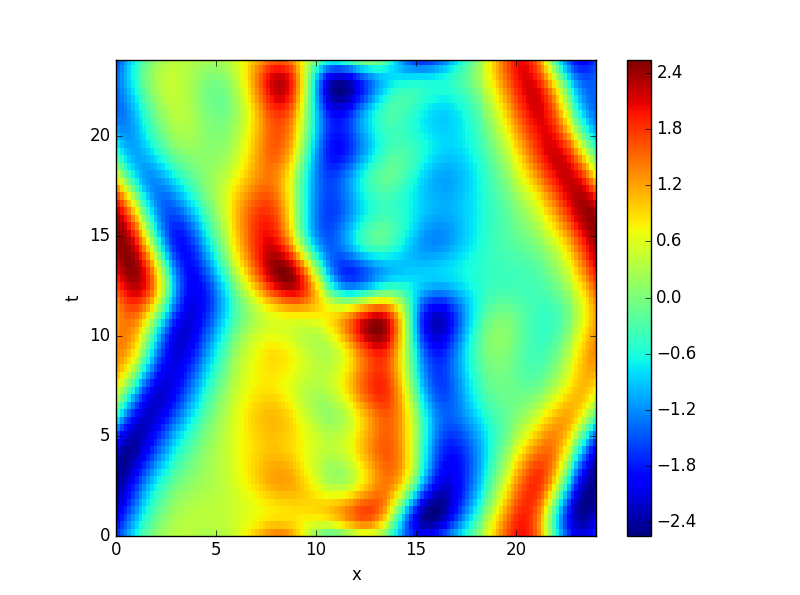
\includegraphics[width=\textwidth,height=.32\textheight]{MNG_st_init}
\end{minipage}
\\
\begin{minipage}[height=.32\textheight]{.45\textwidth}
\centering \small{\texttt{(b)}}
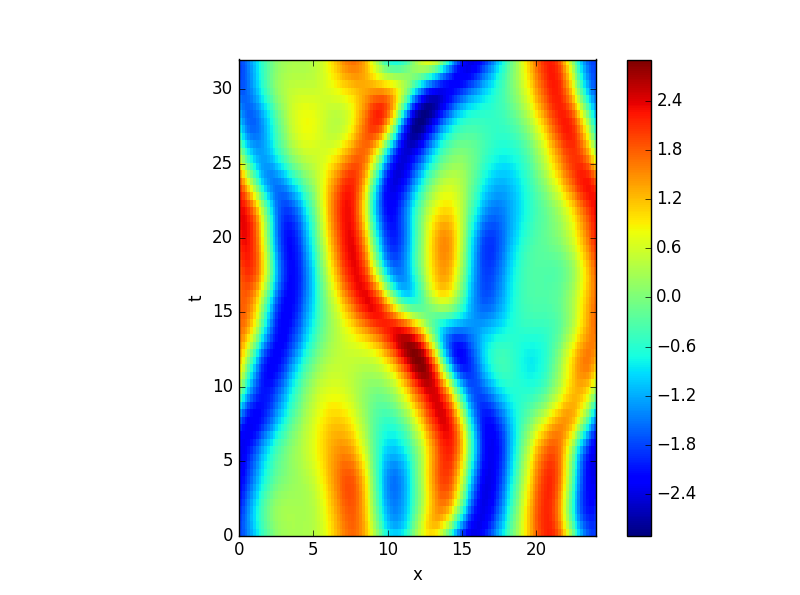
\includegraphics[width=\textwidth,height=.32\textheight]{MNG_st_vnd}
\end{minipage}
\begin{minipage}[height=.32\textheight]{.45\textwidth}
\centering \small{\texttt{(c)}}
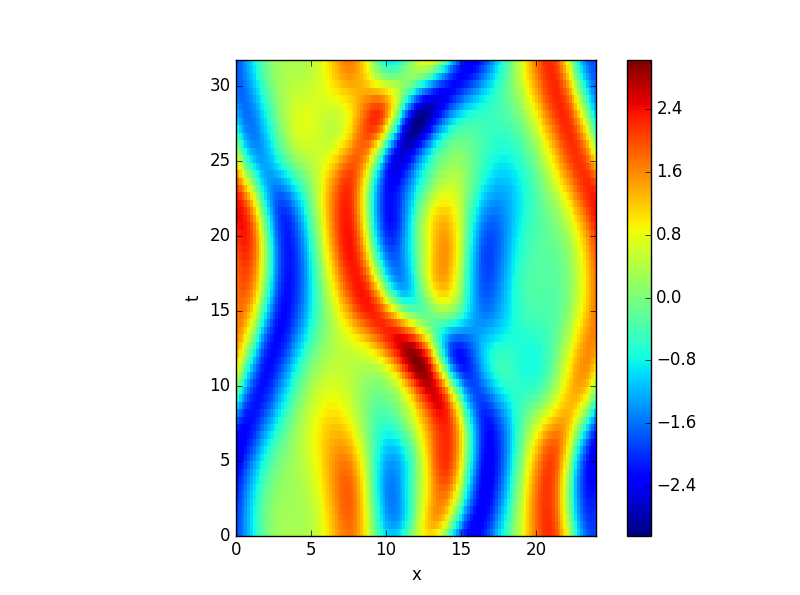
\includegraphics[width=\textwidth,height=.32\textheight]{MNG_st_f}
\end{minipage}
\caption{ \label{fig:MNG_vndst}
(a) The very rough initial condition produced by close recurrence and
intersection of a Poincar\'e hyperplane determined by a {\statesp}
point's reflection $L=24, T=23.8125$.
(b) Where the spatiotemporal initial condition ends up after
variational Newton-descent in time $L=24, T=31.997939649161918$.
(c) The final spatiotemporal fixed point after hybrid adjoint descent
with the reformulation of the preperiodic spatiotemporal mapping, with final domain
size and period $L=24.0714310445$, $T=31.8597201649$
.
}
\end{figure}


\MNGpost{2017-12-14}{
\begin{description}
\item[spatiotemp]
Finally got a machine precision convergence for an arbitrary initial condition (i.e. not one of the solutions
provided by someone else). I believe if I run the adjoint hybrid method long enough and have an accurate enough
initial condition then the convergence is global.

The method uses the adjoint descent and then is followed up with Newton-Krylov hookstep where if the GMRES
solution does not reduce the residual significantly enough then the hookstep is calculated with the conditions
provided by \refref{ChanKers13}. The trust region radius is determined by if the first hookstep in each Newton iteration
is successful in reducing the residual then the radius is doubled, and every time it fails it is reduced by half.

The main issue now is to try to trawl {\statesp} for the best possible initial conditions for the method.

The solution that was found was initialized by finding minima of the $L_2$ norm of a close recurrence procedure
and then the entire spatiotemporal representation was produced by time integration. This next point is probably
going to be the most contentious point I'm going to make, but in order to get a better initial condition for
the full spatiotemporal problem I passed it to the variational {\descent} I had in time to correct the
tangent in time first. I don't think this is being too restrictive because the residual
($L_2$ norm of the spatiotemporal mapping) only changes by one order of magnitude in the original formulation
or two orders of magnitude in the rescaled formulation \refeq{eqn:MNGspacetime_reform}. So, even though it has
been converged in the time-dynamical system sense, it is still many orders of magnitude away from machine
precision residual in the spatiotemporal residual sense.

For comparison, a periodic orbit that is reproduced with known coordinates and time integration would have
a spatiotemporal residual would most likely start around $10^{-6}$ if has been produced well.

The reason I did this was merely to improve the initial conditions. I don't find it to be somehow cheating
because when I pass it to the spatiotemporal problem everything is still allowed to change just in the way
that it was if I had passed the original initial condition to the spatiotemporal problem. This can likely
be conquered by merely producing better initial conditions, which I think can be achieved with more patience
in the process.

Something else I could do is try the adjoint descent in physical space as opposed to Fourier-Fourier space.

\end{description}
}

\MNGpost{2017-12-20}{:
Tried to trawl {\statesp} for initial conditions for my spatiotemporal code and realized that
it ran really slowly for small step sizes (large number of steps). Figured out how to speed
it up by rewriting some key parts of the close recurrence calculations; realized I was sloppy
when it came with the actual optimization previously. Essentially by unrolling some 'for'-loops
and rewriting some key portions I was able to dramatically speed it up.

Instead of the Poincar\'e constraint in addition to close recurrence calculations, which
are in my mind somewhat redundant because I'm trying to compute approximations I instead
played around with a number of different procedures that only relied on close recurrence
calculations, i.e. minimizing the $L_2$ norm of the difference between two {\statesp} points.

Something that I experimented with numerically was a procedure that computed a coarse time-integration
and then if the $L_2$ norm was within a certain tolerance, it would be recomputed with an increased number
of time steps. This would produce great initial conditions in a small number of cases, where the local minima in the
close recurrence diagram actually corresponded to a recurrence, as it would rightly increase the accuracy of both
the starting point of the orbit, the ending point, and the period. I'm sort of deciding between this
and just running one close recurrence trawl with fine integration, because in the majority of cases the
local minima of the $L_2$ norm is just happenstance and not related to a useful recurrence. One of the
symptoms of this is that in certain instances the finer time-integration would actually increase
the minimum of the $L_2$ norm. This didn't make sense to me, and could be due to the exact way I had the
procedure implemented, i.e. taking the minimum from the coarse close recurrence procedure and then
using it as the starting point for the fine close recurrence procedure might be too hopeful, and it might
be best to just start at the same point with the same time range.

So, essentially I sped up the routines to give at least better performance in terms of number of initial
conditions, but the accuracy of such initial conditions could use a little tweaking in terms of bounds
and implementation.

}


\end{description}
%%%%%%%%%%%%%%%%%%%%%%%%%%%%%%%%%%%%%%%%%%%%%%%%%%%%%%%%%%%%%%%%%%%%%%%
\printbibliography[heading=subbibintoc,title={References}]
